\documentclass{coastal_paper}
\usepackage[utf8]{inputenc}
\usepackage{amsmath}
\usepackage{graphicx}
\usepackage{natbib}
\usepackage{textgreek}
\usepackage{lineno}
\usepackage[nolists]{endfloat}
\usepackage{pgfplots}
\usetikzlibrary{external}
\pgfplotsset{compat=1.9}
\usepgfplotslibrary{colorbrewer}
\usepgfplotslibrary{statistics}

\graphicspath{ {./images/fgmax}}
\title{Impacts of Barrier-Island Breaching On Mainland Flooding During Storm Events}
\author{Catherine Jeffries, Robert Weiss, Jennifer Irish, Kyle Mandli}
\begin{document}
\sffamily
\maketitle
\begin{abstract}
Barrier islands can protect the mainland from flooding during storms by affecting the storm surge. However, the protective capability is reduced when barrier islands breach and a direct hydrodynamic connection between the water bodies on both sides of the barrier island is established. Breaching of barrier islands during large storm events is complicated, involving sediment transport and nonlinear processes that connect water and sediment transport, dune height, and island width among other factors. Because of the many factors involved in the breaching process it is difficult to predict where and when a breach will form. In order to assess how barrier-island breaching impacts flooding on the mainland, we use a statistical approach to analyze the sensitivity of mainland storm-surge runup to barrier island breaching by randomizing the location, time, and extent of a breach event. The shape of the breach is approximated with a gaussian distribution imposed on the barrier island that deepens over time. Breach formation is time dependent after a triggering event, for preliminary work specified as 1 m of flow depth over the barrier island, during a simulated storm event using GeoClaw, and breach growth is limited by the flow conditions in its rate of change and when it achieves equilibrium. Varying the timing, extent, and locations of the barrier island breaches during a storm event will provide insight into how the mainland coastline responds to breaches during storms. This insight is invaluable in preparing shoreline communities to be aware of the differing ways the regions can change during storms, depending on how the barrier islands behave. Additionally, we can offer statistical insights into where a breach would impact the mainland coastline more drastically in an effort to provide data for planning and warning purposes.    
\end{abstract}
\newpage

\linenumbers
\section{Introduction}
Barrier islands are elongate, shore-parallel, low-relief land masses that are adjacent to approximately 6.5\% of the world's coastlines \citep{Oertel1985TheSystem,Stutz2001ADistribution}. \citet{Oertel1985TheSystem} defines barrier island systems as containing six sedimentary environments; proximity to the mainland, a back-barrier region (bay or lagoon), an inlet and inlet delta, the barrier island, the barrier platform, and the shoreface. Barrier islands are protective structures that assist with dissipating the wave energy approaching the mainland from the ocean. The dissipation of wave energy ensures that barrier islands undergo significant change during storms and hurricanes, one of which is breaching. A breach is an opening in a narrow landmass, such as a barrier island, that allows a direct hydrodynamic connection between the ocean and the back-barrier bay or lagoon \citep{Kraus2003, Kraus2003a, Wamsley2005CoastalClosure, KRAUS2005}. Breaching that occurs naturally is a complicated process that combines waves, overwash, barrier island width and height, and storm forcing to initiate. 

Large storms, such as hurricanes, can have a devastating impact on barrier islands and the mainland coastline. One of the many hazards presented by such storms is storm surge, a forced wave driven by wind and atmospheric pressure changes during the hurricane. Storm surge that causes a water level gradient between the ocean and back-barrier region will force water to flow rapidly over the barrier island and erode the sediment of the island in an effort to equalize the water level. This gradient involves a critical elevation of water levels that may not necessarily involve inundation of the island, but can still cause erosion \citep{Kraus2002, Kraus2003}. Storm surge and wave setup both increase the elevation of the water in the ocean and the back-barrier region; these water levels in addition to wave action reduce the stability of the barrier island dune slope \citep{Kraus2003, Kraus2002}. However, wave attack by itself, while weakening the dune slope, is unlikely to induce breaching because the net erosion is seaward and does not push erosion landward \citep{Pierce1970}. Breaching can occur through two different transport methods, overtopping (overwash) and seepage and liquefaction \citep{Kraus2002, Kraus2003}.

During storm-induced overwash and inundation of the islands, the water flowing across the island can scour a channel between the sea and the back-barrier region \citep{Kraus2003, Pierce1970, Roelvink2009}. For this scouring to occur a strong flow and some duration of inundation are required. Breaching can occur from both the seaward and landward side of the barrier island but field data is limited in its ability to illustrate from which direction a breach is initiated \citep{Kraus2003, Pierce1970, Smallegan2017}. However, \citet{Smallegan2017} show that bay surge that comes after peak ocean surge is more likely to lead to breaching from the landward side of the barrier island. This is due to peak ocean surge having already weakened the dune through erosion caused by wave attack and swash \citep{Kraus2003, Smallegan2017}. Breach location is challenging to correctly identify; localized lows in dune height and narrower portions of the barrier island are more likely to be potential breach locations \citep{Kraus2003, Kraus2003a}. \citet{Vander2019} simulated Hurricane Sandy (2012) with both wave forcing and sediment transport to illustrate barrier island morphodynamics during the hurricane and correctly modeled a breach but the location was simulated to be some distance away from where the breach was located in reality. 

Breach dimensions are difficult to quantify, the growth of breaches over time has been documented \citep{Kraus2003a, Schmeltz1983Breach/InletInlet.}. However, these studies address the days, weeks, or months following the storm. Initial breach size during a storm is less known. Lab and field experiments by \citet{Visser1999} for breaches in dikes are useful but the breach is initiated with a pre-drilled hole in the dike and does not simulate exactly what occurs to barrier islands during storms. \citet{Buynevich2006} performed a geologic mapping of some New England barrier islands and found geoloci signatures to indicate the islands' past history with breaching and overwash. They found ephemeral breaches with widths of 10 - 30 m before closing and breach depths of 1-3 meters below the dune crest. A few post-storm surveys have defined breach sizes before natural or forced closing. \cite{Kraus2003a} discusses Pike's inlet on Long Island, NY was initially 304.8 m wide and a nearby breach named Little Pike's inlet was initially 30.48 m wide but over several months grew to over 914.4 m before it was closed. A breach near Moriches Inlet studied by \cite{Schmeltz1983Breach/InletInlet.} has an initial size of 91.4 m and 0.61 m depth. This breach expanded to 885 m with a 3 m depth before it was closed by the US Army Corps of Engineers (USACE). The uncertainties in breach dimensions and  in where, how, and when breaches occur remains one of the many issues facing coastal communities today.

Barrier islands exist along the coasts of 18 states that border the Atlantic Ocean and Gulf of Mexico \citep{Zhang2011}. As coastal populations have increased considerably over the last few decades, the protective nature of barrier islands have become even more important \citep{Zhang2011}. The National Hurricane Center (NHC) states that storm surge  is the largest contributor to life loss and property damage during hurricanes \citep{Center2006}. During a hurricane, storm surge induces flooding that can damage structures, close roads, and impact the lives of humans living in the coastal zone. Storm surge can also speed up erosion on both barrier islands and the mainland coast, which then can drive more flooding. Understanding how barrier island breaching affects coastal flooding from storm surge is important for risk assessment and mitigation efforts. The opening of a hydrodynamic connection between the ocean and the back-barrier region can lead to increased flooding and waves during hurricanes that increases the risk to populations and property. However, there is little information currently available on how different breach morphodynamics affect the mainland.

In this paper, we explore a method of simulating barrier island breach in order to evaluate the impacts of storm surge induced breaching on mainland flooding. Using a storm modeling software, GeoClaw, we artificially alter the bathymetry of a barrier island to create a breach. This process provides a more controlled method of simulating breaching than using a sediment transport model. We remove the complexities involved in the sediment transport in order to purely study the mainland's flood response to a breach opening in random locations along the barrier island and at different times during the storm simulation. 

\section{Methods}

Our goal for this project is to quantify the differences in coastal and bay flooding if breaching occurs during a hurricane. To simulate the storm we are running simulations with GeoClaw a subsidiary of Clawpack, a suite of conservation law programs that solve hyperbolic differential equations in 1 and 2 dimensions to model geophysical events \citep{clawpack, mandli2016clawpack}. Clawpack employs adaptive mesh refinement (AMR) that allows for increasing resolution where and when it is needed and reduces the computational overhead while providing an accurate solution \citep{Berger2011TheRefinement}. GeoClaw calculates storm surge with a 2 dimensional depth averaged model that solves the classical shallow water equations with source terms for bathymetry, bottom friction, Coriolis forcing, surface pressure, and wind friction \citep{Mandli2014}. 

Breaching is a complex process that is difficult to accurately model, the storm forcing, width of the island, sediment transport, and other complex processes are all involved that make it difficult to predict where and when a breach will occur. To accomplish our goal of quantifying flooding due to breaching we chose to simplify breaching by reducing the topography of the barrier island at specific locations. We simulate a breach using an approximation of a gaussian function to provide a breach with sloping sides and the deepest part in the center. During the storm simulation we apply \ref{eq:breach_gaussian} to reduce the height of the barrier island at a selected location, where $\mu$ is the center of the breach location, $d^t$ is the height of the breach location at time t, X is the longitude of the location being reduced and $t_T$ is a timing factor that controls how quickly the breach opens. The timing factor for these simulations allow for the breach to open fully in an hour after \citet{Visser1999}.
\begin{equation}
    d^t = d^{t-1} - e^{-\frac{1}{2}{(X - \mu)^2}}t_T
    \label{eq:breach_gaussian}
\end{equation}

The storm we employ to simulate storm surge is a proxy for the 1938 New England hurricane. The storm data was generated for the US Army Corps of Engineers (USACE) North Atlantic Comprehensive Coast Survey (NACCS) \citep{cialone2015north}. The storm forcing is provided by wind and pressure fields that have data in 15 minute increments. Accurate modeling of this storm requires sub-minute data and AMR requires data to be integrated at increasing resolution where needed. To provide the sub-minute time steps we use linear interpolation of the wind and pressure fields, to define the wind and pressure forcing inside the AMR grids we employ bi-linear interpolation when and where it is required. The chosen storm has a similar track and intensity of the 1938 hurricane. We can verify the accuracy of the solution with a tide gauge at Sandy Hook, NJ that has data recorded from 1938, once adjustments are made for modern bathymetry and sea levels. The bathymetry we obtained for Moriches, NY is from NOAA's continuously updated 1/9 arc second topobathy dataset, for the basin we used GEBCO 30 arc second \citep{cires2014continuously, weatherall2015new}.

The 1938 hurricane at Moriches, NY caused six breaches, three west of the inlet and three east of the inlet; quantifying the bay and coastal flooding changes during this hurricane requires that we vary the locations, timing, width, and depth of these breaches and recording the differences in synthetic tide gauges placed around the bay and recording maximum water levels in a large grid that is resolved to 18 meters. A no breach scenario provided the baselines we used for quantifying differences in breaching scenarios and verifying a breaching location is viable. We simulated synthetic tide gauges on the seaward side of the bay as a proxy for island inundation. Once a breach location is chosen we verify it is viable by taking the synthetic tide gauges within one km of the breach and calculate that the tide gauge reaches a minimum of 24\% of the dune height. If no gauges within one km reach that water height we choose a new location and start the test over. This allows for a reasonable estimate of the conditions that could induce breaching, if the water levels just offshore do not reach a critical height it is unlikely a breach would open at that location.

We started with the original six breach dimensions as estimated from \citet{Canizares2008}, from there we created a monte-carlo framework that employs a random uniform distribution for both breach width and depth. For the first set of simulations we held the depth steady at -2.0 meters and varied the widths for each breach individually between 25 - 630 meters. Our second set of scenarios, we kept the original 1938 breach width estimations and varied the depths between 0 and -2.0 meters. The endpoints for each randomization was chosen from examples in the literature \citep{Schmeltz1983Breach/InletInlet., Kraus2003a,Visser1999, Canizares2008}. The time of initiation for each breach was chosen using the nearest synthetic tide gauge data from a no breach simulation; the first time in seconds the nearest tide gauge reaches 24\% of the maximum dune height at each location was our start time. We chose to have the breaches fully open within one hour after initiation.

We evaluated our results using the maximum surge height data recorded by GeoClaw for the entire bay. Splitting the bay into 3 sections, east, central, and west, then comparing the varying width vs. depth simulations to identify if one parameter has more impact on bay flooding than another. Additionally, we calculated the change in wet vs. dry cells amongst the simulations and compared them to the original no breach simulation to quantify the area of inundation that occurs per scenario.
% find a way to explain the single scenarios for volume of water through breach, or total breach area

\section{Results}
To analyse the results we looked at both surge height at random points in the bay and total inundation in square meters. For the randomly chosen locations we split the bay into thirds, for each section (west, central, east) we show  the mean of the surge height is higher for the depth variations, but the width scenarios have a larger variance. When varying both width and depth, the surge height is correlated to the number of breaches more than the mean breach area.

\begin{figure}
    \centering
    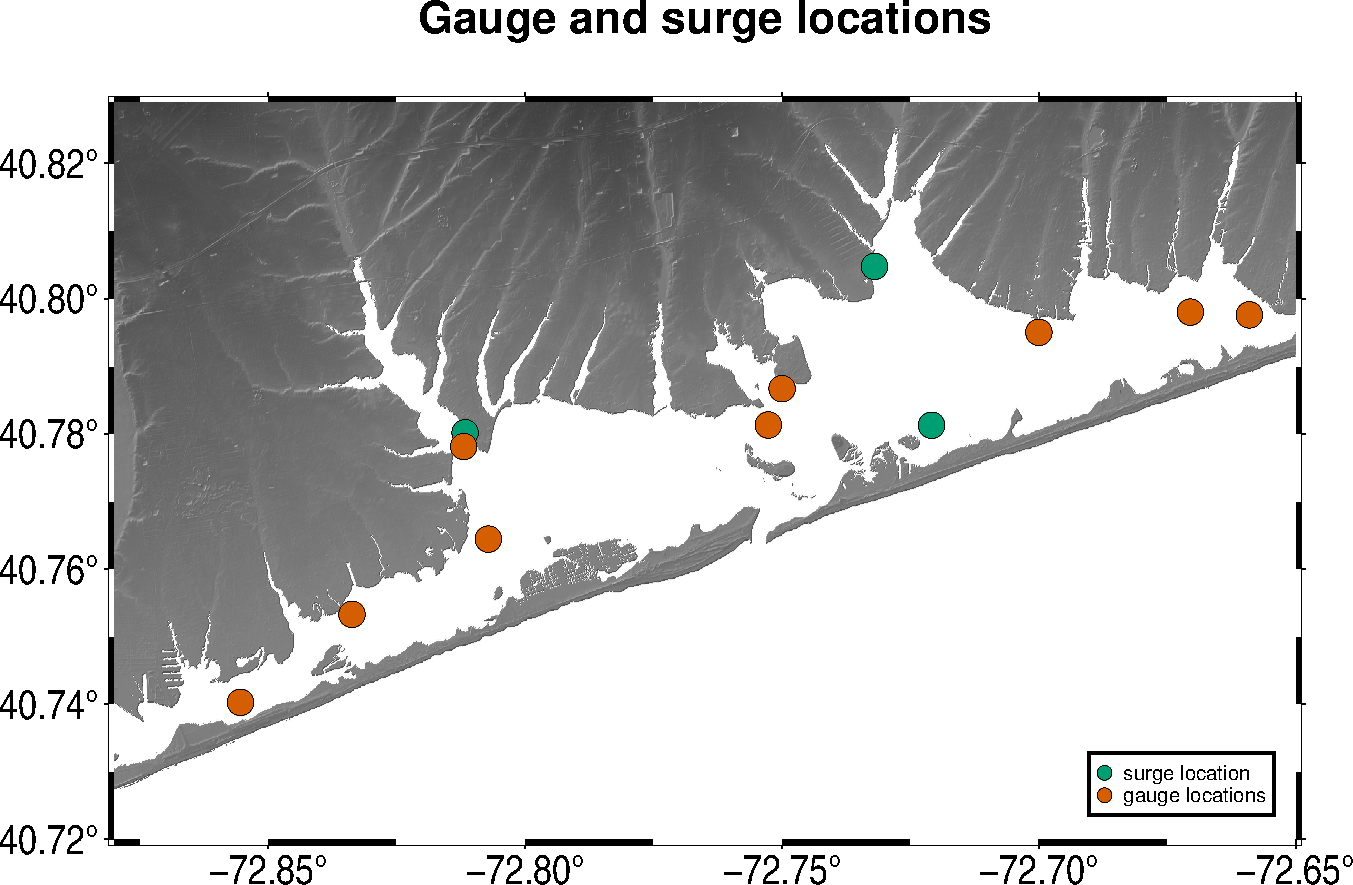
\includegraphics[width=0.75\textwidth]{images/dot_map.pdf}
    \caption{Location of storm surge points (green) in Moriches, NY}
    \label{fig1}
\end{figure}

\begin{figure}[ht]
\centering
%% Creator: Matplotlib, PGF backend
%%
%% To include the figure in your LaTeX document, write
%%   \input{<filename>.pgf}
%%
%% Make sure the required packages are loaded in your preamble
%%   \usepackage{pgf}
%%
%% Also ensure that all the required font packages are loaded; for instance,
%% the lmodern package is sometimes necessary when using math font.
%%   \usepackage{lmodern}
%%
%% Figures using additional raster images can only be included by \input if
%% they are in the same directory as the main LaTeX file. For loading figures
%% from other directories you can use the `import` package
%%   \usepackage{import}
%%
%% and then include the figures with
%%   \import{<path to file>}{<filename>.pgf}
%%
%% Matplotlib used the following preamble
%%   \usepackage{fontspec}
%%
\begingroup%
\makeatletter%
\begin{pgfpicture}%
\pgfpathrectangle{\pgfpointorigin}{\pgfqpoint{8.637284in}{3.176611in}}%
\pgfusepath{use as bounding box, clip}%
\begin{pgfscope}%
\pgfsetbuttcap%
\pgfsetmiterjoin%
\definecolor{currentfill}{rgb}{1.000000,1.000000,1.000000}%
\pgfsetfillcolor{currentfill}%
\pgfsetlinewidth{0.000000pt}%
\definecolor{currentstroke}{rgb}{1.000000,1.000000,1.000000}%
\pgfsetstrokecolor{currentstroke}%
\pgfsetdash{}{0pt}%
\pgfpathmoveto{\pgfqpoint{-0.000000in}{0.000000in}}%
\pgfpathlineto{\pgfqpoint{8.637284in}{0.000000in}}%
\pgfpathlineto{\pgfqpoint{8.637284in}{3.176611in}}%
\pgfpathlineto{\pgfqpoint{-0.000000in}{3.176611in}}%
\pgfpathlineto{\pgfqpoint{-0.000000in}{0.000000in}}%
\pgfpathclose%
\pgfusepath{fill}%
\end{pgfscope}%
\begin{pgfscope}%
\pgfsetbuttcap%
\pgfsetmiterjoin%
\definecolor{currentfill}{rgb}{1.000000,1.000000,1.000000}%
\pgfsetfillcolor{currentfill}%
\pgfsetlinewidth{0.000000pt}%
\definecolor{currentstroke}{rgb}{0.000000,0.000000,0.000000}%
\pgfsetstrokecolor{currentstroke}%
\pgfsetstrokeopacity{0.000000}%
\pgfsetdash{}{0pt}%
\pgfpathmoveto{\pgfqpoint{0.444137in}{0.529055in}}%
\pgfpathlineto{\pgfqpoint{2.723548in}{0.529055in}}%
\pgfpathlineto{\pgfqpoint{2.723548in}{2.839055in}}%
\pgfpathlineto{\pgfqpoint{0.444137in}{2.839055in}}%
\pgfpathlineto{\pgfqpoint{0.444137in}{0.529055in}}%
\pgfpathclose%
\pgfusepath{fill}%
\end{pgfscope}%
\begin{pgfscope}%
\pgfpathrectangle{\pgfqpoint{0.444137in}{0.529055in}}{\pgfqpoint{2.279412in}{2.310000in}}%
\pgfusepath{clip}%
\pgfsetbuttcap%
\pgfsetmiterjoin%
\definecolor{currentfill}{rgb}{0.835294,0.368627,0.000000}%
\pgfsetfillcolor{currentfill}%
\pgfsetfillopacity{0.200000}%
\pgfsetlinewidth{0.803000pt}%
\definecolor{currentstroke}{rgb}{0.000000,0.000000,0.000000}%
\pgfsetstrokecolor{currentstroke}%
\pgfsetstrokeopacity{0.200000}%
\pgfsetdash{}{0pt}%
\pgfpathmoveto{\pgfqpoint{1.044500in}{0.529055in}}%
\pgfpathlineto{\pgfqpoint{1.044500in}{1.092944in}}%
\pgfpathlineto{\pgfqpoint{1.102869in}{1.092944in}}%
\pgfpathlineto{\pgfqpoint{1.102869in}{1.092944in}}%
\pgfpathlineto{\pgfqpoint{1.161238in}{1.092944in}}%
\pgfpathlineto{\pgfqpoint{1.161238in}{0.742944in}}%
\pgfpathlineto{\pgfqpoint{1.219607in}{0.742944in}}%
\pgfpathlineto{\pgfqpoint{1.219607in}{0.781833in}}%
\pgfpathlineto{\pgfqpoint{1.277976in}{0.781833in}}%
\pgfpathlineto{\pgfqpoint{1.277976in}{0.820722in}}%
\pgfpathlineto{\pgfqpoint{1.336345in}{0.820722in}}%
\pgfpathlineto{\pgfqpoint{1.336345in}{0.995722in}}%
\pgfpathlineto{\pgfqpoint{1.394714in}{0.995722in}}%
\pgfpathlineto{\pgfqpoint{1.394714in}{0.956833in}}%
\pgfpathlineto{\pgfqpoint{1.453082in}{0.956833in}}%
\pgfpathlineto{\pgfqpoint{1.453082in}{1.034611in}}%
\pgfpathlineto{\pgfqpoint{1.511451in}{1.034611in}}%
\pgfpathlineto{\pgfqpoint{1.511451in}{1.073500in}}%
\pgfpathlineto{\pgfqpoint{1.569820in}{1.073500in}}%
\pgfpathlineto{\pgfqpoint{1.569820in}{0.937388in}}%
\pgfpathlineto{\pgfqpoint{1.628189in}{0.937388in}}%
\pgfpathlineto{\pgfqpoint{1.628189in}{0.879055in}}%
\pgfpathlineto{\pgfqpoint{1.686558in}{0.879055in}}%
\pgfpathlineto{\pgfqpoint{1.686558in}{0.937388in}}%
\pgfpathlineto{\pgfqpoint{1.744927in}{0.937388in}}%
\pgfpathlineto{\pgfqpoint{1.744927in}{0.742944in}}%
\pgfpathlineto{\pgfqpoint{1.803296in}{0.742944in}}%
\pgfpathlineto{\pgfqpoint{1.803296in}{0.684611in}}%
\pgfpathlineto{\pgfqpoint{1.861665in}{0.684611in}}%
\pgfpathlineto{\pgfqpoint{1.861665in}{0.781833in}}%
\pgfpathlineto{\pgfqpoint{1.920034in}{0.781833in}}%
\pgfpathlineto{\pgfqpoint{1.920034in}{0.665166in}}%
\pgfpathlineto{\pgfqpoint{1.978403in}{0.665166in}}%
\pgfpathlineto{\pgfqpoint{1.978403in}{0.548500in}}%
\pgfpathlineto{\pgfqpoint{2.036771in}{0.548500in}}%
\pgfpathlineto{\pgfqpoint{2.036771in}{0.529055in}}%
\pgfpathlineto{\pgfqpoint{2.095140in}{0.529055in}}%
\pgfpathlineto{\pgfqpoint{2.095140in}{0.529055in}}%
\pgfpathlineto{\pgfqpoint{2.153509in}{0.529055in}}%
\pgfpathlineto{\pgfqpoint{2.153509in}{0.529055in}}%
\pgfpathlineto{\pgfqpoint{2.211878in}{0.529055in}}%
\pgfpathlineto{\pgfqpoint{2.211878in}{0.529055in}}%
\pgfpathlineto{\pgfqpoint{2.153509in}{0.529055in}}%
\pgfpathlineto{\pgfqpoint{2.153509in}{0.529055in}}%
\pgfpathlineto{\pgfqpoint{2.095140in}{0.529055in}}%
\pgfpathlineto{\pgfqpoint{2.095140in}{0.529055in}}%
\pgfpathlineto{\pgfqpoint{2.036771in}{0.529055in}}%
\pgfpathlineto{\pgfqpoint{2.036771in}{0.529055in}}%
\pgfpathlineto{\pgfqpoint{1.978403in}{0.529055in}}%
\pgfpathlineto{\pgfqpoint{1.978403in}{0.529055in}}%
\pgfpathlineto{\pgfqpoint{1.920034in}{0.529055in}}%
\pgfpathlineto{\pgfqpoint{1.920034in}{0.529055in}}%
\pgfpathlineto{\pgfqpoint{1.861665in}{0.529055in}}%
\pgfpathlineto{\pgfqpoint{1.861665in}{0.529055in}}%
\pgfpathlineto{\pgfqpoint{1.803296in}{0.529055in}}%
\pgfpathlineto{\pgfqpoint{1.803296in}{0.529055in}}%
\pgfpathlineto{\pgfqpoint{1.744927in}{0.529055in}}%
\pgfpathlineto{\pgfqpoint{1.744927in}{0.529055in}}%
\pgfpathlineto{\pgfqpoint{1.686558in}{0.529055in}}%
\pgfpathlineto{\pgfqpoint{1.686558in}{0.529055in}}%
\pgfpathlineto{\pgfqpoint{1.628189in}{0.529055in}}%
\pgfpathlineto{\pgfqpoint{1.628189in}{0.529055in}}%
\pgfpathlineto{\pgfqpoint{1.569820in}{0.529055in}}%
\pgfpathlineto{\pgfqpoint{1.569820in}{0.529055in}}%
\pgfpathlineto{\pgfqpoint{1.511451in}{0.529055in}}%
\pgfpathlineto{\pgfqpoint{1.511451in}{0.529055in}}%
\pgfpathlineto{\pgfqpoint{1.453082in}{0.529055in}}%
\pgfpathlineto{\pgfqpoint{1.453082in}{0.529055in}}%
\pgfpathlineto{\pgfqpoint{1.394714in}{0.529055in}}%
\pgfpathlineto{\pgfqpoint{1.394714in}{0.529055in}}%
\pgfpathlineto{\pgfqpoint{1.336345in}{0.529055in}}%
\pgfpathlineto{\pgfqpoint{1.336345in}{0.529055in}}%
\pgfpathlineto{\pgfqpoint{1.277976in}{0.529055in}}%
\pgfpathlineto{\pgfqpoint{1.277976in}{0.529055in}}%
\pgfpathlineto{\pgfqpoint{1.219607in}{0.529055in}}%
\pgfpathlineto{\pgfqpoint{1.219607in}{0.529055in}}%
\pgfpathlineto{\pgfqpoint{1.161238in}{0.529055in}}%
\pgfpathlineto{\pgfqpoint{1.161238in}{0.529055in}}%
\pgfpathlineto{\pgfqpoint{1.102869in}{0.529055in}}%
\pgfpathlineto{\pgfqpoint{1.102869in}{0.529055in}}%
\pgfpathlineto{\pgfqpoint{1.044500in}{0.529055in}}%
\pgfpathclose%
\pgfusepath{stroke,fill}%
\end{pgfscope}%
\begin{pgfscope}%
\pgfpathrectangle{\pgfqpoint{0.444137in}{0.529055in}}{\pgfqpoint{2.279412in}{2.310000in}}%
\pgfusepath{clip}%
\pgfsetbuttcap%
\pgfsetmiterjoin%
\definecolor{currentfill}{rgb}{0.000000,0.619608,0.450980}%
\pgfsetfillcolor{currentfill}%
\pgfsetfillopacity{0.200000}%
\pgfsetlinewidth{0.803000pt}%
\definecolor{currentstroke}{rgb}{0.000000,0.000000,0.000000}%
\pgfsetstrokecolor{currentstroke}%
\pgfsetstrokeopacity{0.200000}%
\pgfsetdash{}{0pt}%
\pgfpathmoveto{\pgfqpoint{1.044500in}{0.529055in}}%
\pgfpathlineto{\pgfqpoint{1.044500in}{0.529055in}}%
\pgfpathlineto{\pgfqpoint{1.102869in}{0.529055in}}%
\pgfpathlineto{\pgfqpoint{1.102869in}{0.529055in}}%
\pgfpathlineto{\pgfqpoint{1.161238in}{0.529055in}}%
\pgfpathlineto{\pgfqpoint{1.161238in}{0.529055in}}%
\pgfpathlineto{\pgfqpoint{1.219607in}{0.529055in}}%
\pgfpathlineto{\pgfqpoint{1.219607in}{0.529055in}}%
\pgfpathlineto{\pgfqpoint{1.277976in}{0.529055in}}%
\pgfpathlineto{\pgfqpoint{1.277976in}{0.591286in}}%
\pgfpathlineto{\pgfqpoint{1.336345in}{0.591286in}}%
\pgfpathlineto{\pgfqpoint{1.336345in}{0.628624in}}%
\pgfpathlineto{\pgfqpoint{1.394714in}{0.628624in}}%
\pgfpathlineto{\pgfqpoint{1.394714in}{0.740639in}}%
\pgfpathlineto{\pgfqpoint{1.453082in}{0.740639in}}%
\pgfpathlineto{\pgfqpoint{1.453082in}{1.039346in}}%
\pgfpathlineto{\pgfqpoint{1.511451in}{1.039346in}}%
\pgfpathlineto{\pgfqpoint{1.511451in}{1.101577in}}%
\pgfpathlineto{\pgfqpoint{1.569820in}{1.101577in}}%
\pgfpathlineto{\pgfqpoint{1.569820in}{1.201146in}}%
\pgfpathlineto{\pgfqpoint{1.628189in}{1.201146in}}%
\pgfpathlineto{\pgfqpoint{1.628189in}{1.300715in}}%
\pgfpathlineto{\pgfqpoint{1.686558in}{1.300715in}}%
\pgfpathlineto{\pgfqpoint{1.686558in}{1.089131in}}%
\pgfpathlineto{\pgfqpoint{1.744927in}{1.089131in}}%
\pgfpathlineto{\pgfqpoint{1.744927in}{0.840208in}}%
\pgfpathlineto{\pgfqpoint{1.803296in}{0.840208in}}%
\pgfpathlineto{\pgfqpoint{1.803296in}{0.802870in}}%
\pgfpathlineto{\pgfqpoint{1.861665in}{0.802870in}}%
\pgfpathlineto{\pgfqpoint{1.861665in}{0.952223in}}%
\pgfpathlineto{\pgfqpoint{1.920034in}{0.952223in}}%
\pgfpathlineto{\pgfqpoint{1.920034in}{0.840208in}}%
\pgfpathlineto{\pgfqpoint{1.978403in}{0.840208in}}%
\pgfpathlineto{\pgfqpoint{1.978403in}{0.827762in}}%
\pgfpathlineto{\pgfqpoint{2.036771in}{0.827762in}}%
\pgfpathlineto{\pgfqpoint{2.036771in}{0.939777in}}%
\pgfpathlineto{\pgfqpoint{2.095140in}{0.939777in}}%
\pgfpathlineto{\pgfqpoint{2.095140in}{0.765531in}}%
\pgfpathlineto{\pgfqpoint{2.153509in}{0.765531in}}%
\pgfpathlineto{\pgfqpoint{2.153509in}{0.578840in}}%
\pgfpathlineto{\pgfqpoint{2.211878in}{0.578840in}}%
\pgfpathlineto{\pgfqpoint{2.211878in}{0.529055in}}%
\pgfpathlineto{\pgfqpoint{2.153509in}{0.529055in}}%
\pgfpathlineto{\pgfqpoint{2.153509in}{0.529055in}}%
\pgfpathlineto{\pgfqpoint{2.095140in}{0.529055in}}%
\pgfpathlineto{\pgfqpoint{2.095140in}{0.529055in}}%
\pgfpathlineto{\pgfqpoint{2.036771in}{0.529055in}}%
\pgfpathlineto{\pgfqpoint{2.036771in}{0.529055in}}%
\pgfpathlineto{\pgfqpoint{1.978403in}{0.529055in}}%
\pgfpathlineto{\pgfqpoint{1.978403in}{0.529055in}}%
\pgfpathlineto{\pgfqpoint{1.920034in}{0.529055in}}%
\pgfpathlineto{\pgfqpoint{1.920034in}{0.529055in}}%
\pgfpathlineto{\pgfqpoint{1.861665in}{0.529055in}}%
\pgfpathlineto{\pgfqpoint{1.861665in}{0.529055in}}%
\pgfpathlineto{\pgfqpoint{1.803296in}{0.529055in}}%
\pgfpathlineto{\pgfqpoint{1.803296in}{0.529055in}}%
\pgfpathlineto{\pgfqpoint{1.744927in}{0.529055in}}%
\pgfpathlineto{\pgfqpoint{1.744927in}{0.529055in}}%
\pgfpathlineto{\pgfqpoint{1.686558in}{0.529055in}}%
\pgfpathlineto{\pgfqpoint{1.686558in}{0.529055in}}%
\pgfpathlineto{\pgfqpoint{1.628189in}{0.529055in}}%
\pgfpathlineto{\pgfqpoint{1.628189in}{0.529055in}}%
\pgfpathlineto{\pgfqpoint{1.569820in}{0.529055in}}%
\pgfpathlineto{\pgfqpoint{1.569820in}{0.529055in}}%
\pgfpathlineto{\pgfqpoint{1.511451in}{0.529055in}}%
\pgfpathlineto{\pgfqpoint{1.511451in}{0.529055in}}%
\pgfpathlineto{\pgfqpoint{1.453082in}{0.529055in}}%
\pgfpathlineto{\pgfqpoint{1.453082in}{0.529055in}}%
\pgfpathlineto{\pgfqpoint{1.394714in}{0.529055in}}%
\pgfpathlineto{\pgfqpoint{1.394714in}{0.529055in}}%
\pgfpathlineto{\pgfqpoint{1.336345in}{0.529055in}}%
\pgfpathlineto{\pgfqpoint{1.336345in}{0.529055in}}%
\pgfpathlineto{\pgfqpoint{1.277976in}{0.529055in}}%
\pgfpathlineto{\pgfqpoint{1.277976in}{0.529055in}}%
\pgfpathlineto{\pgfqpoint{1.219607in}{0.529055in}}%
\pgfpathlineto{\pgfqpoint{1.219607in}{0.529055in}}%
\pgfpathlineto{\pgfqpoint{1.161238in}{0.529055in}}%
\pgfpathlineto{\pgfqpoint{1.161238in}{0.529055in}}%
\pgfpathlineto{\pgfqpoint{1.102869in}{0.529055in}}%
\pgfpathlineto{\pgfqpoint{1.102869in}{0.529055in}}%
\pgfpathlineto{\pgfqpoint{1.044500in}{0.529055in}}%
\pgfpathclose%
\pgfusepath{stroke,fill}%
\end{pgfscope}%
\begin{pgfscope}%
\pgfpathrectangle{\pgfqpoint{0.444137in}{0.529055in}}{\pgfqpoint{2.279412in}{2.310000in}}%
\pgfusepath{clip}%
\pgfsetbuttcap%
\pgfsetmiterjoin%
\definecolor{currentfill}{rgb}{0.337255,0.705882,0.913725}%
\pgfsetfillcolor{currentfill}%
\pgfsetfillopacity{0.200000}%
\pgfsetlinewidth{0.803000pt}%
\definecolor{currentstroke}{rgb}{0.000000,0.000000,0.000000}%
\pgfsetstrokecolor{currentstroke}%
\pgfsetstrokeopacity{0.200000}%
\pgfsetdash{}{0pt}%
\pgfpathmoveto{\pgfqpoint{1.044500in}{0.529055in}}%
\pgfpathlineto{\pgfqpoint{1.044500in}{0.529055in}}%
\pgfpathlineto{\pgfqpoint{1.102869in}{0.529055in}}%
\pgfpathlineto{\pgfqpoint{1.102869in}{0.529055in}}%
\pgfpathlineto{\pgfqpoint{1.161238in}{0.529055in}}%
\pgfpathlineto{\pgfqpoint{1.161238in}{0.529055in}}%
\pgfpathlineto{\pgfqpoint{1.219607in}{0.529055in}}%
\pgfpathlineto{\pgfqpoint{1.219607in}{0.529055in}}%
\pgfpathlineto{\pgfqpoint{1.277976in}{0.529055in}}%
\pgfpathlineto{\pgfqpoint{1.277976in}{0.529055in}}%
\pgfpathlineto{\pgfqpoint{1.336345in}{0.529055in}}%
\pgfpathlineto{\pgfqpoint{1.336345in}{0.529055in}}%
\pgfpathlineto{\pgfqpoint{1.394714in}{0.529055in}}%
\pgfpathlineto{\pgfqpoint{1.394714in}{0.529055in}}%
\pgfpathlineto{\pgfqpoint{1.453082in}{0.529055in}}%
\pgfpathlineto{\pgfqpoint{1.453082in}{0.529055in}}%
\pgfpathlineto{\pgfqpoint{1.511451in}{0.529055in}}%
\pgfpathlineto{\pgfqpoint{1.511451in}{0.529055in}}%
\pgfpathlineto{\pgfqpoint{1.569820in}{0.529055in}}%
\pgfpathlineto{\pgfqpoint{1.569820in}{0.529055in}}%
\pgfpathlineto{\pgfqpoint{1.628189in}{0.529055in}}%
\pgfpathlineto{\pgfqpoint{1.628189in}{0.542675in}}%
\pgfpathlineto{\pgfqpoint{1.686558in}{0.542675in}}%
\pgfpathlineto{\pgfqpoint{1.686558in}{0.583536in}}%
\pgfpathlineto{\pgfqpoint{1.744927in}{0.583536in}}%
\pgfpathlineto{\pgfqpoint{1.744927in}{0.855942in}}%
\pgfpathlineto{\pgfqpoint{1.803296in}{0.855942in}}%
\pgfpathlineto{\pgfqpoint{1.803296in}{1.005765in}}%
\pgfpathlineto{\pgfqpoint{1.861665in}{1.005765in}}%
\pgfpathlineto{\pgfqpoint{1.861665in}{1.073866in}}%
\pgfpathlineto{\pgfqpoint{1.920034in}{1.073866in}}%
\pgfpathlineto{\pgfqpoint{1.920034in}{1.128348in}}%
\pgfpathlineto{\pgfqpoint{1.978403in}{1.128348in}}%
\pgfpathlineto{\pgfqpoint{1.978403in}{1.427994in}}%
\pgfpathlineto{\pgfqpoint{2.036771in}{1.427994in}}%
\pgfpathlineto{\pgfqpoint{2.036771in}{1.972805in}}%
\pgfpathlineto{\pgfqpoint{2.095140in}{1.972805in}}%
\pgfpathlineto{\pgfqpoint{2.095140in}{1.931944in}}%
\pgfpathlineto{\pgfqpoint{2.153509in}{1.931944in}}%
\pgfpathlineto{\pgfqpoint{2.153509in}{0.542675in}}%
\pgfpathlineto{\pgfqpoint{2.211878in}{0.542675in}}%
\pgfpathlineto{\pgfqpoint{2.211878in}{0.529055in}}%
\pgfpathlineto{\pgfqpoint{2.153509in}{0.529055in}}%
\pgfpathlineto{\pgfqpoint{2.153509in}{0.529055in}}%
\pgfpathlineto{\pgfqpoint{2.095140in}{0.529055in}}%
\pgfpathlineto{\pgfqpoint{2.095140in}{0.529055in}}%
\pgfpathlineto{\pgfqpoint{2.036771in}{0.529055in}}%
\pgfpathlineto{\pgfqpoint{2.036771in}{0.529055in}}%
\pgfpathlineto{\pgfqpoint{1.978403in}{0.529055in}}%
\pgfpathlineto{\pgfqpoint{1.978403in}{0.529055in}}%
\pgfpathlineto{\pgfqpoint{1.920034in}{0.529055in}}%
\pgfpathlineto{\pgfqpoint{1.920034in}{0.529055in}}%
\pgfpathlineto{\pgfqpoint{1.861665in}{0.529055in}}%
\pgfpathlineto{\pgfqpoint{1.861665in}{0.529055in}}%
\pgfpathlineto{\pgfqpoint{1.803296in}{0.529055in}}%
\pgfpathlineto{\pgfqpoint{1.803296in}{0.529055in}}%
\pgfpathlineto{\pgfqpoint{1.744927in}{0.529055in}}%
\pgfpathlineto{\pgfqpoint{1.744927in}{0.529055in}}%
\pgfpathlineto{\pgfqpoint{1.686558in}{0.529055in}}%
\pgfpathlineto{\pgfqpoint{1.686558in}{0.529055in}}%
\pgfpathlineto{\pgfqpoint{1.628189in}{0.529055in}}%
\pgfpathlineto{\pgfqpoint{1.628189in}{0.529055in}}%
\pgfpathlineto{\pgfqpoint{1.569820in}{0.529055in}}%
\pgfpathlineto{\pgfqpoint{1.569820in}{0.529055in}}%
\pgfpathlineto{\pgfqpoint{1.511451in}{0.529055in}}%
\pgfpathlineto{\pgfqpoint{1.511451in}{0.529055in}}%
\pgfpathlineto{\pgfqpoint{1.453082in}{0.529055in}}%
\pgfpathlineto{\pgfqpoint{1.453082in}{0.529055in}}%
\pgfpathlineto{\pgfqpoint{1.394714in}{0.529055in}}%
\pgfpathlineto{\pgfqpoint{1.394714in}{0.529055in}}%
\pgfpathlineto{\pgfqpoint{1.336345in}{0.529055in}}%
\pgfpathlineto{\pgfqpoint{1.336345in}{0.529055in}}%
\pgfpathlineto{\pgfqpoint{1.277976in}{0.529055in}}%
\pgfpathlineto{\pgfqpoint{1.277976in}{0.529055in}}%
\pgfpathlineto{\pgfqpoint{1.219607in}{0.529055in}}%
\pgfpathlineto{\pgfqpoint{1.219607in}{0.529055in}}%
\pgfpathlineto{\pgfqpoint{1.161238in}{0.529055in}}%
\pgfpathlineto{\pgfqpoint{1.161238in}{0.529055in}}%
\pgfpathlineto{\pgfqpoint{1.102869in}{0.529055in}}%
\pgfpathlineto{\pgfqpoint{1.102869in}{0.529055in}}%
\pgfpathlineto{\pgfqpoint{1.044500in}{0.529055in}}%
\pgfpathclose%
\pgfusepath{stroke,fill}%
\end{pgfscope}%
\begin{pgfscope}%
\pgfsetbuttcap%
\pgfsetroundjoin%
\definecolor{currentfill}{rgb}{0.196078,0.188235,0.203922}%
\pgfsetfillcolor{currentfill}%
\pgfsetlinewidth{0.803000pt}%
\definecolor{currentstroke}{rgb}{0.196078,0.188235,0.203922}%
\pgfsetstrokecolor{currentstroke}%
\pgfsetdash{}{0pt}%
\pgfsys@defobject{currentmarker}{\pgfqpoint{0.000000in}{-0.048611in}}{\pgfqpoint{0.000000in}{0.000000in}}{%
\pgfpathmoveto{\pgfqpoint{0.000000in}{0.000000in}}%
\pgfpathlineto{\pgfqpoint{0.000000in}{-0.048611in}}%
\pgfusepath{stroke,fill}%
}%
\begin{pgfscope}%
\pgfsys@transformshift{0.444137in}{0.529055in}%
\pgfsys@useobject{currentmarker}{}%
\end{pgfscope}%
\end{pgfscope}%
\begin{pgfscope}%
\definecolor{textcolor}{rgb}{0.196078,0.188235,0.203922}%
\pgfsetstrokecolor{textcolor}%
\pgfsetfillcolor{textcolor}%
\pgftext[x=0.444137in,y=0.431833in,,top]{\color{textcolor}\rmfamily\fontsize{10.000000}{12.000000}\selectfont 0.55}%
\end{pgfscope}%
\begin{pgfscope}%
\pgfsetbuttcap%
\pgfsetroundjoin%
\definecolor{currentfill}{rgb}{0.196078,0.188235,0.203922}%
\pgfsetfillcolor{currentfill}%
\pgfsetlinewidth{0.803000pt}%
\definecolor{currentstroke}{rgb}{0.196078,0.188235,0.203922}%
\pgfsetstrokecolor{currentstroke}%
\pgfsetdash{}{0pt}%
\pgfsys@defobject{currentmarker}{\pgfqpoint{0.000000in}{-0.048611in}}{\pgfqpoint{0.000000in}{0.000000in}}{%
\pgfpathmoveto{\pgfqpoint{0.000000in}{0.000000in}}%
\pgfpathlineto{\pgfqpoint{0.000000in}{-0.048611in}}%
\pgfusepath{stroke,fill}%
}%
\begin{pgfscope}%
\pgfsys@transformshift{0.769767in}{0.529055in}%
\pgfsys@useobject{currentmarker}{}%
\end{pgfscope}%
\end{pgfscope}%
\begin{pgfscope}%
\definecolor{textcolor}{rgb}{0.196078,0.188235,0.203922}%
\pgfsetstrokecolor{textcolor}%
\pgfsetfillcolor{textcolor}%
\pgftext[x=0.769767in,y=0.431833in,,top]{\color{textcolor}\rmfamily\fontsize{10.000000}{12.000000}\selectfont 0.66}%
\end{pgfscope}%
\begin{pgfscope}%
\pgfsetbuttcap%
\pgfsetroundjoin%
\definecolor{currentfill}{rgb}{0.196078,0.188235,0.203922}%
\pgfsetfillcolor{currentfill}%
\pgfsetlinewidth{0.803000pt}%
\definecolor{currentstroke}{rgb}{0.196078,0.188235,0.203922}%
\pgfsetstrokecolor{currentstroke}%
\pgfsetdash{}{0pt}%
\pgfsys@defobject{currentmarker}{\pgfqpoint{0.000000in}{-0.048611in}}{\pgfqpoint{0.000000in}{0.000000in}}{%
\pgfpathmoveto{\pgfqpoint{0.000000in}{0.000000in}}%
\pgfpathlineto{\pgfqpoint{0.000000in}{-0.048611in}}%
\pgfusepath{stroke,fill}%
}%
\begin{pgfscope}%
\pgfsys@transformshift{1.095397in}{0.529055in}%
\pgfsys@useobject{currentmarker}{}%
\end{pgfscope}%
\end{pgfscope}%
\begin{pgfscope}%
\definecolor{textcolor}{rgb}{0.196078,0.188235,0.203922}%
\pgfsetstrokecolor{textcolor}%
\pgfsetfillcolor{textcolor}%
\pgftext[x=1.095397in,y=0.431833in,,top]{\color{textcolor}\rmfamily\fontsize{10.000000}{12.000000}\selectfont 0.76}%
\end{pgfscope}%
\begin{pgfscope}%
\pgfsetbuttcap%
\pgfsetroundjoin%
\definecolor{currentfill}{rgb}{0.196078,0.188235,0.203922}%
\pgfsetfillcolor{currentfill}%
\pgfsetlinewidth{0.803000pt}%
\definecolor{currentstroke}{rgb}{0.196078,0.188235,0.203922}%
\pgfsetstrokecolor{currentstroke}%
\pgfsetdash{}{0pt}%
\pgfsys@defobject{currentmarker}{\pgfqpoint{0.000000in}{-0.048611in}}{\pgfqpoint{0.000000in}{0.000000in}}{%
\pgfpathmoveto{\pgfqpoint{0.000000in}{0.000000in}}%
\pgfpathlineto{\pgfqpoint{0.000000in}{-0.048611in}}%
\pgfusepath{stroke,fill}%
}%
\begin{pgfscope}%
\pgfsys@transformshift{1.421027in}{0.529055in}%
\pgfsys@useobject{currentmarker}{}%
\end{pgfscope}%
\end{pgfscope}%
\begin{pgfscope}%
\definecolor{textcolor}{rgb}{0.196078,0.188235,0.203922}%
\pgfsetstrokecolor{textcolor}%
\pgfsetfillcolor{textcolor}%
\pgftext[x=1.421027in,y=0.431833in,,top]{\color{textcolor}\rmfamily\fontsize{10.000000}{12.000000}\selectfont 0.87}%
\end{pgfscope}%
\begin{pgfscope}%
\pgfsetbuttcap%
\pgfsetroundjoin%
\definecolor{currentfill}{rgb}{0.196078,0.188235,0.203922}%
\pgfsetfillcolor{currentfill}%
\pgfsetlinewidth{0.803000pt}%
\definecolor{currentstroke}{rgb}{0.196078,0.188235,0.203922}%
\pgfsetstrokecolor{currentstroke}%
\pgfsetdash{}{0pt}%
\pgfsys@defobject{currentmarker}{\pgfqpoint{0.000000in}{-0.048611in}}{\pgfqpoint{0.000000in}{0.000000in}}{%
\pgfpathmoveto{\pgfqpoint{0.000000in}{0.000000in}}%
\pgfpathlineto{\pgfqpoint{0.000000in}{-0.048611in}}%
\pgfusepath{stroke,fill}%
}%
\begin{pgfscope}%
\pgfsys@transformshift{1.746658in}{0.529055in}%
\pgfsys@useobject{currentmarker}{}%
\end{pgfscope}%
\end{pgfscope}%
\begin{pgfscope}%
\definecolor{textcolor}{rgb}{0.196078,0.188235,0.203922}%
\pgfsetstrokecolor{textcolor}%
\pgfsetfillcolor{textcolor}%
\pgftext[x=1.746658in,y=0.431833in,,top]{\color{textcolor}\rmfamily\fontsize{10.000000}{12.000000}\selectfont 0.98}%
\end{pgfscope}%
\begin{pgfscope}%
\pgfsetbuttcap%
\pgfsetroundjoin%
\definecolor{currentfill}{rgb}{0.196078,0.188235,0.203922}%
\pgfsetfillcolor{currentfill}%
\pgfsetlinewidth{0.803000pt}%
\definecolor{currentstroke}{rgb}{0.196078,0.188235,0.203922}%
\pgfsetstrokecolor{currentstroke}%
\pgfsetdash{}{0pt}%
\pgfsys@defobject{currentmarker}{\pgfqpoint{0.000000in}{-0.048611in}}{\pgfqpoint{0.000000in}{0.000000in}}{%
\pgfpathmoveto{\pgfqpoint{0.000000in}{0.000000in}}%
\pgfpathlineto{\pgfqpoint{0.000000in}{-0.048611in}}%
\pgfusepath{stroke,fill}%
}%
\begin{pgfscope}%
\pgfsys@transformshift{2.072288in}{0.529055in}%
\pgfsys@useobject{currentmarker}{}%
\end{pgfscope}%
\end{pgfscope}%
\begin{pgfscope}%
\definecolor{textcolor}{rgb}{0.196078,0.188235,0.203922}%
\pgfsetstrokecolor{textcolor}%
\pgfsetfillcolor{textcolor}%
\pgftext[x=2.072288in,y=0.431833in,,top]{\color{textcolor}\rmfamily\fontsize{10.000000}{12.000000}\selectfont 1.09}%
\end{pgfscope}%
\begin{pgfscope}%
\pgfsetbuttcap%
\pgfsetroundjoin%
\definecolor{currentfill}{rgb}{0.196078,0.188235,0.203922}%
\pgfsetfillcolor{currentfill}%
\pgfsetlinewidth{0.803000pt}%
\definecolor{currentstroke}{rgb}{0.196078,0.188235,0.203922}%
\pgfsetstrokecolor{currentstroke}%
\pgfsetdash{}{0pt}%
\pgfsys@defobject{currentmarker}{\pgfqpoint{0.000000in}{-0.048611in}}{\pgfqpoint{0.000000in}{0.000000in}}{%
\pgfpathmoveto{\pgfqpoint{0.000000in}{0.000000in}}%
\pgfpathlineto{\pgfqpoint{0.000000in}{-0.048611in}}%
\pgfusepath{stroke,fill}%
}%
\begin{pgfscope}%
\pgfsys@transformshift{2.397918in}{0.529055in}%
\pgfsys@useobject{currentmarker}{}%
\end{pgfscope}%
\end{pgfscope}%
\begin{pgfscope}%
\definecolor{textcolor}{rgb}{0.196078,0.188235,0.203922}%
\pgfsetstrokecolor{textcolor}%
\pgfsetfillcolor{textcolor}%
\pgftext[x=2.397918in,y=0.431833in,,top]{\color{textcolor}\rmfamily\fontsize{10.000000}{12.000000}\selectfont 1.19}%
\end{pgfscope}%
\begin{pgfscope}%
\pgfsetbuttcap%
\pgfsetroundjoin%
\definecolor{currentfill}{rgb}{0.196078,0.188235,0.203922}%
\pgfsetfillcolor{currentfill}%
\pgfsetlinewidth{0.803000pt}%
\definecolor{currentstroke}{rgb}{0.196078,0.188235,0.203922}%
\pgfsetstrokecolor{currentstroke}%
\pgfsetdash{}{0pt}%
\pgfsys@defobject{currentmarker}{\pgfqpoint{0.000000in}{-0.048611in}}{\pgfqpoint{0.000000in}{0.000000in}}{%
\pgfpathmoveto{\pgfqpoint{0.000000in}{0.000000in}}%
\pgfpathlineto{\pgfqpoint{0.000000in}{-0.048611in}}%
\pgfusepath{stroke,fill}%
}%
\begin{pgfscope}%
\pgfsys@transformshift{2.723548in}{0.529055in}%
\pgfsys@useobject{currentmarker}{}%
\end{pgfscope}%
\end{pgfscope}%
\begin{pgfscope}%
\definecolor{textcolor}{rgb}{0.196078,0.188235,0.203922}%
\pgfsetstrokecolor{textcolor}%
\pgfsetfillcolor{textcolor}%
\pgftext[x=2.723548in,y=0.431833in,,top]{\color{textcolor}\rmfamily\fontsize{10.000000}{12.000000}\selectfont 1.30}%
\end{pgfscope}%
\begin{pgfscope}%
\pgfsetbuttcap%
\pgfsetroundjoin%
\definecolor{currentfill}{rgb}{0.196078,0.188235,0.203922}%
\pgfsetfillcolor{currentfill}%
\pgfsetlinewidth{0.803000pt}%
\definecolor{currentstroke}{rgb}{0.196078,0.188235,0.203922}%
\pgfsetstrokecolor{currentstroke}%
\pgfsetdash{}{0pt}%
\pgfsys@defobject{currentmarker}{\pgfqpoint{-0.048611in}{0.000000in}}{\pgfqpoint{-0.000000in}{0.000000in}}{%
\pgfpathmoveto{\pgfqpoint{-0.000000in}{0.000000in}}%
\pgfpathlineto{\pgfqpoint{-0.048611in}{0.000000in}}%
\pgfusepath{stroke,fill}%
}%
\begin{pgfscope}%
\pgfsys@transformshift{0.444137in}{0.529055in}%
\pgfsys@useobject{currentmarker}{}%
\end{pgfscope}%
\end{pgfscope}%
\begin{pgfscope}%
\definecolor{textcolor}{rgb}{0.196078,0.188235,0.203922}%
\pgfsetstrokecolor{textcolor}%
\pgfsetfillcolor{textcolor}%
\pgftext[x=0.100000in, y=0.480861in, left, base]{\color{textcolor}\rmfamily\fontsize{10.000000}{12.000000}\selectfont \(\displaystyle {0.00}\)}%
\end{pgfscope}%
\begin{pgfscope}%
\pgfsetbuttcap%
\pgfsetroundjoin%
\definecolor{currentfill}{rgb}{0.196078,0.188235,0.203922}%
\pgfsetfillcolor{currentfill}%
\pgfsetlinewidth{0.803000pt}%
\definecolor{currentstroke}{rgb}{0.196078,0.188235,0.203922}%
\pgfsetstrokecolor{currentstroke}%
\pgfsetdash{}{0pt}%
\pgfsys@defobject{currentmarker}{\pgfqpoint{-0.048611in}{0.000000in}}{\pgfqpoint{-0.000000in}{0.000000in}}{%
\pgfpathmoveto{\pgfqpoint{-0.000000in}{0.000000in}}%
\pgfpathlineto{\pgfqpoint{-0.048611in}{0.000000in}}%
\pgfusepath{stroke,fill}%
}%
\begin{pgfscope}%
\pgfsys@transformshift{0.444137in}{0.817805in}%
\pgfsys@useobject{currentmarker}{}%
\end{pgfscope}%
\end{pgfscope}%
\begin{pgfscope}%
\definecolor{textcolor}{rgb}{0.196078,0.188235,0.203922}%
\pgfsetstrokecolor{textcolor}%
\pgfsetfillcolor{textcolor}%
\pgftext[x=0.100000in, y=0.769611in, left, base]{\color{textcolor}\rmfamily\fontsize{10.000000}{12.000000}\selectfont \(\displaystyle {0.05}\)}%
\end{pgfscope}%
\begin{pgfscope}%
\pgfsetbuttcap%
\pgfsetroundjoin%
\definecolor{currentfill}{rgb}{0.196078,0.188235,0.203922}%
\pgfsetfillcolor{currentfill}%
\pgfsetlinewidth{0.803000pt}%
\definecolor{currentstroke}{rgb}{0.196078,0.188235,0.203922}%
\pgfsetstrokecolor{currentstroke}%
\pgfsetdash{}{0pt}%
\pgfsys@defobject{currentmarker}{\pgfqpoint{-0.048611in}{0.000000in}}{\pgfqpoint{-0.000000in}{0.000000in}}{%
\pgfpathmoveto{\pgfqpoint{-0.000000in}{0.000000in}}%
\pgfpathlineto{\pgfqpoint{-0.048611in}{0.000000in}}%
\pgfusepath{stroke,fill}%
}%
\begin{pgfscope}%
\pgfsys@transformshift{0.444137in}{1.106555in}%
\pgfsys@useobject{currentmarker}{}%
\end{pgfscope}%
\end{pgfscope}%
\begin{pgfscope}%
\definecolor{textcolor}{rgb}{0.196078,0.188235,0.203922}%
\pgfsetstrokecolor{textcolor}%
\pgfsetfillcolor{textcolor}%
\pgftext[x=0.100000in, y=1.058361in, left, base]{\color{textcolor}\rmfamily\fontsize{10.000000}{12.000000}\selectfont \(\displaystyle {0.10}\)}%
\end{pgfscope}%
\begin{pgfscope}%
\pgfsetbuttcap%
\pgfsetroundjoin%
\definecolor{currentfill}{rgb}{0.196078,0.188235,0.203922}%
\pgfsetfillcolor{currentfill}%
\pgfsetlinewidth{0.803000pt}%
\definecolor{currentstroke}{rgb}{0.196078,0.188235,0.203922}%
\pgfsetstrokecolor{currentstroke}%
\pgfsetdash{}{0pt}%
\pgfsys@defobject{currentmarker}{\pgfqpoint{-0.048611in}{0.000000in}}{\pgfqpoint{-0.000000in}{0.000000in}}{%
\pgfpathmoveto{\pgfqpoint{-0.000000in}{0.000000in}}%
\pgfpathlineto{\pgfqpoint{-0.048611in}{0.000000in}}%
\pgfusepath{stroke,fill}%
}%
\begin{pgfscope}%
\pgfsys@transformshift{0.444137in}{1.395305in}%
\pgfsys@useobject{currentmarker}{}%
\end{pgfscope}%
\end{pgfscope}%
\begin{pgfscope}%
\definecolor{textcolor}{rgb}{0.196078,0.188235,0.203922}%
\pgfsetstrokecolor{textcolor}%
\pgfsetfillcolor{textcolor}%
\pgftext[x=0.100000in, y=1.347111in, left, base]{\color{textcolor}\rmfamily\fontsize{10.000000}{12.000000}\selectfont \(\displaystyle {0.15}\)}%
\end{pgfscope}%
\begin{pgfscope}%
\pgfsetbuttcap%
\pgfsetroundjoin%
\definecolor{currentfill}{rgb}{0.196078,0.188235,0.203922}%
\pgfsetfillcolor{currentfill}%
\pgfsetlinewidth{0.803000pt}%
\definecolor{currentstroke}{rgb}{0.196078,0.188235,0.203922}%
\pgfsetstrokecolor{currentstroke}%
\pgfsetdash{}{0pt}%
\pgfsys@defobject{currentmarker}{\pgfqpoint{-0.048611in}{0.000000in}}{\pgfqpoint{-0.000000in}{0.000000in}}{%
\pgfpathmoveto{\pgfqpoint{-0.000000in}{0.000000in}}%
\pgfpathlineto{\pgfqpoint{-0.048611in}{0.000000in}}%
\pgfusepath{stroke,fill}%
}%
\begin{pgfscope}%
\pgfsys@transformshift{0.444137in}{1.684055in}%
\pgfsys@useobject{currentmarker}{}%
\end{pgfscope}%
\end{pgfscope}%
\begin{pgfscope}%
\definecolor{textcolor}{rgb}{0.196078,0.188235,0.203922}%
\pgfsetstrokecolor{textcolor}%
\pgfsetfillcolor{textcolor}%
\pgftext[x=0.100000in, y=1.635861in, left, base]{\color{textcolor}\rmfamily\fontsize{10.000000}{12.000000}\selectfont \(\displaystyle {0.20}\)}%
\end{pgfscope}%
\begin{pgfscope}%
\pgfsetbuttcap%
\pgfsetroundjoin%
\definecolor{currentfill}{rgb}{0.196078,0.188235,0.203922}%
\pgfsetfillcolor{currentfill}%
\pgfsetlinewidth{0.803000pt}%
\definecolor{currentstroke}{rgb}{0.196078,0.188235,0.203922}%
\pgfsetstrokecolor{currentstroke}%
\pgfsetdash{}{0pt}%
\pgfsys@defobject{currentmarker}{\pgfqpoint{-0.048611in}{0.000000in}}{\pgfqpoint{-0.000000in}{0.000000in}}{%
\pgfpathmoveto{\pgfqpoint{-0.000000in}{0.000000in}}%
\pgfpathlineto{\pgfqpoint{-0.048611in}{0.000000in}}%
\pgfusepath{stroke,fill}%
}%
\begin{pgfscope}%
\pgfsys@transformshift{0.444137in}{1.972805in}%
\pgfsys@useobject{currentmarker}{}%
\end{pgfscope}%
\end{pgfscope}%
\begin{pgfscope}%
\definecolor{textcolor}{rgb}{0.196078,0.188235,0.203922}%
\pgfsetstrokecolor{textcolor}%
\pgfsetfillcolor{textcolor}%
\pgftext[x=0.100000in, y=1.924611in, left, base]{\color{textcolor}\rmfamily\fontsize{10.000000}{12.000000}\selectfont \(\displaystyle {0.25}\)}%
\end{pgfscope}%
\begin{pgfscope}%
\pgfsetbuttcap%
\pgfsetroundjoin%
\definecolor{currentfill}{rgb}{0.196078,0.188235,0.203922}%
\pgfsetfillcolor{currentfill}%
\pgfsetlinewidth{0.803000pt}%
\definecolor{currentstroke}{rgb}{0.196078,0.188235,0.203922}%
\pgfsetstrokecolor{currentstroke}%
\pgfsetdash{}{0pt}%
\pgfsys@defobject{currentmarker}{\pgfqpoint{-0.048611in}{0.000000in}}{\pgfqpoint{-0.000000in}{0.000000in}}{%
\pgfpathmoveto{\pgfqpoint{-0.000000in}{0.000000in}}%
\pgfpathlineto{\pgfqpoint{-0.048611in}{0.000000in}}%
\pgfusepath{stroke,fill}%
}%
\begin{pgfscope}%
\pgfsys@transformshift{0.444137in}{2.261555in}%
\pgfsys@useobject{currentmarker}{}%
\end{pgfscope}%
\end{pgfscope}%
\begin{pgfscope}%
\definecolor{textcolor}{rgb}{0.196078,0.188235,0.203922}%
\pgfsetstrokecolor{textcolor}%
\pgfsetfillcolor{textcolor}%
\pgftext[x=0.100000in, y=2.213361in, left, base]{\color{textcolor}\rmfamily\fontsize{10.000000}{12.000000}\selectfont \(\displaystyle {0.30}\)}%
\end{pgfscope}%
\begin{pgfscope}%
\pgfsetbuttcap%
\pgfsetroundjoin%
\definecolor{currentfill}{rgb}{0.196078,0.188235,0.203922}%
\pgfsetfillcolor{currentfill}%
\pgfsetlinewidth{0.803000pt}%
\definecolor{currentstroke}{rgb}{0.196078,0.188235,0.203922}%
\pgfsetstrokecolor{currentstroke}%
\pgfsetdash{}{0pt}%
\pgfsys@defobject{currentmarker}{\pgfqpoint{-0.048611in}{0.000000in}}{\pgfqpoint{-0.000000in}{0.000000in}}{%
\pgfpathmoveto{\pgfqpoint{-0.000000in}{0.000000in}}%
\pgfpathlineto{\pgfqpoint{-0.048611in}{0.000000in}}%
\pgfusepath{stroke,fill}%
}%
\begin{pgfscope}%
\pgfsys@transformshift{0.444137in}{2.550305in}%
\pgfsys@useobject{currentmarker}{}%
\end{pgfscope}%
\end{pgfscope}%
\begin{pgfscope}%
\definecolor{textcolor}{rgb}{0.196078,0.188235,0.203922}%
\pgfsetstrokecolor{textcolor}%
\pgfsetfillcolor{textcolor}%
\pgftext[x=0.100000in, y=2.502111in, left, base]{\color{textcolor}\rmfamily\fontsize{10.000000}{12.000000}\selectfont \(\displaystyle {0.35}\)}%
\end{pgfscope}%
\begin{pgfscope}%
\pgfsetbuttcap%
\pgfsetroundjoin%
\definecolor{currentfill}{rgb}{0.196078,0.188235,0.203922}%
\pgfsetfillcolor{currentfill}%
\pgfsetlinewidth{0.803000pt}%
\definecolor{currentstroke}{rgb}{0.196078,0.188235,0.203922}%
\pgfsetstrokecolor{currentstroke}%
\pgfsetdash{}{0pt}%
\pgfsys@defobject{currentmarker}{\pgfqpoint{-0.048611in}{0.000000in}}{\pgfqpoint{-0.000000in}{0.000000in}}{%
\pgfpathmoveto{\pgfqpoint{-0.000000in}{0.000000in}}%
\pgfpathlineto{\pgfqpoint{-0.048611in}{0.000000in}}%
\pgfusepath{stroke,fill}%
}%
\begin{pgfscope}%
\pgfsys@transformshift{0.444137in}{2.839055in}%
\pgfsys@useobject{currentmarker}{}%
\end{pgfscope}%
\end{pgfscope}%
\begin{pgfscope}%
\definecolor{textcolor}{rgb}{0.196078,0.188235,0.203922}%
\pgfsetstrokecolor{textcolor}%
\pgfsetfillcolor{textcolor}%
\pgftext[x=0.100000in, y=2.790861in, left, base]{\color{textcolor}\rmfamily\fontsize{10.000000}{12.000000}\selectfont \(\displaystyle {0.40}\)}%
\end{pgfscope}%
\begin{pgfscope}%
\pgfpathrectangle{\pgfqpoint{0.444137in}{0.529055in}}{\pgfqpoint{2.279412in}{2.310000in}}%
\pgfusepath{clip}%
\pgfsetbuttcap%
\pgfsetmiterjoin%
\pgfsetlinewidth{0.803000pt}%
\definecolor{currentstroke}{rgb}{0.835294,0.368627,0.000000}%
\pgfsetstrokecolor{currentstroke}%
\pgfsetstrokeopacity{0.700000}%
\pgfsetdash{}{0pt}%
\pgfpathmoveto{\pgfqpoint{1.044500in}{0.529055in}}%
\pgfpathlineto{\pgfqpoint{1.044500in}{1.092944in}}%
\pgfpathlineto{\pgfqpoint{1.102869in}{1.092944in}}%
\pgfpathlineto{\pgfqpoint{1.102869in}{1.092944in}}%
\pgfpathlineto{\pgfqpoint{1.161238in}{1.092944in}}%
\pgfpathlineto{\pgfqpoint{1.161238in}{0.742944in}}%
\pgfpathlineto{\pgfqpoint{1.219607in}{0.742944in}}%
\pgfpathlineto{\pgfqpoint{1.219607in}{0.781833in}}%
\pgfpathlineto{\pgfqpoint{1.277976in}{0.781833in}}%
\pgfpathlineto{\pgfqpoint{1.277976in}{0.820722in}}%
\pgfpathlineto{\pgfqpoint{1.336345in}{0.820722in}}%
\pgfpathlineto{\pgfqpoint{1.336345in}{0.995722in}}%
\pgfpathlineto{\pgfqpoint{1.394714in}{0.995722in}}%
\pgfpathlineto{\pgfqpoint{1.394714in}{0.956833in}}%
\pgfpathlineto{\pgfqpoint{1.453082in}{0.956833in}}%
\pgfpathlineto{\pgfqpoint{1.453082in}{1.034611in}}%
\pgfpathlineto{\pgfqpoint{1.511451in}{1.034611in}}%
\pgfpathlineto{\pgfqpoint{1.511451in}{1.073500in}}%
\pgfpathlineto{\pgfqpoint{1.569820in}{1.073500in}}%
\pgfpathlineto{\pgfqpoint{1.569820in}{0.937388in}}%
\pgfpathlineto{\pgfqpoint{1.628189in}{0.937388in}}%
\pgfpathlineto{\pgfqpoint{1.628189in}{0.879055in}}%
\pgfpathlineto{\pgfqpoint{1.686558in}{0.879055in}}%
\pgfpathlineto{\pgfqpoint{1.686558in}{0.937388in}}%
\pgfpathlineto{\pgfqpoint{1.744927in}{0.937388in}}%
\pgfpathlineto{\pgfqpoint{1.744927in}{0.742944in}}%
\pgfpathlineto{\pgfqpoint{1.803296in}{0.742944in}}%
\pgfpathlineto{\pgfqpoint{1.803296in}{0.684611in}}%
\pgfpathlineto{\pgfqpoint{1.861665in}{0.684611in}}%
\pgfpathlineto{\pgfqpoint{1.861665in}{0.781833in}}%
\pgfpathlineto{\pgfqpoint{1.920034in}{0.781833in}}%
\pgfpathlineto{\pgfqpoint{1.920034in}{0.665166in}}%
\pgfpathlineto{\pgfqpoint{1.978403in}{0.665166in}}%
\pgfpathlineto{\pgfqpoint{1.978403in}{0.548500in}}%
\pgfpathlineto{\pgfqpoint{2.036771in}{0.548500in}}%
\pgfpathlineto{\pgfqpoint{2.036771in}{0.529055in}}%
\pgfpathlineto{\pgfqpoint{2.095140in}{0.529055in}}%
\pgfpathlineto{\pgfqpoint{2.095140in}{0.529055in}}%
\pgfpathlineto{\pgfqpoint{2.153509in}{0.529055in}}%
\pgfpathlineto{\pgfqpoint{2.153509in}{0.529055in}}%
\pgfpathlineto{\pgfqpoint{2.211878in}{0.529055in}}%
\pgfpathlineto{\pgfqpoint{2.211878in}{0.529055in}}%
\pgfusepath{stroke}%
\end{pgfscope}%
\begin{pgfscope}%
\pgfpathrectangle{\pgfqpoint{0.444137in}{0.529055in}}{\pgfqpoint{2.279412in}{2.310000in}}%
\pgfusepath{clip}%
\pgfsetbuttcap%
\pgfsetmiterjoin%
\pgfsetlinewidth{0.803000pt}%
\definecolor{currentstroke}{rgb}{0.000000,0.619608,0.450980}%
\pgfsetstrokecolor{currentstroke}%
\pgfsetstrokeopacity{0.700000}%
\pgfsetdash{}{0pt}%
\pgfpathmoveto{\pgfqpoint{1.044500in}{0.529055in}}%
\pgfpathlineto{\pgfqpoint{1.044500in}{0.529055in}}%
\pgfpathlineto{\pgfqpoint{1.102869in}{0.529055in}}%
\pgfpathlineto{\pgfqpoint{1.102869in}{0.529055in}}%
\pgfpathlineto{\pgfqpoint{1.161238in}{0.529055in}}%
\pgfpathlineto{\pgfqpoint{1.161238in}{0.529055in}}%
\pgfpathlineto{\pgfqpoint{1.219607in}{0.529055in}}%
\pgfpathlineto{\pgfqpoint{1.219607in}{0.529055in}}%
\pgfpathlineto{\pgfqpoint{1.277976in}{0.529055in}}%
\pgfpathlineto{\pgfqpoint{1.277976in}{0.591286in}}%
\pgfpathlineto{\pgfqpoint{1.336345in}{0.591286in}}%
\pgfpathlineto{\pgfqpoint{1.336345in}{0.628624in}}%
\pgfpathlineto{\pgfqpoint{1.394714in}{0.628624in}}%
\pgfpathlineto{\pgfqpoint{1.394714in}{0.740639in}}%
\pgfpathlineto{\pgfqpoint{1.453082in}{0.740639in}}%
\pgfpathlineto{\pgfqpoint{1.453082in}{1.039346in}}%
\pgfpathlineto{\pgfqpoint{1.511451in}{1.039346in}}%
\pgfpathlineto{\pgfqpoint{1.511451in}{1.101577in}}%
\pgfpathlineto{\pgfqpoint{1.569820in}{1.101577in}}%
\pgfpathlineto{\pgfqpoint{1.569820in}{1.201146in}}%
\pgfpathlineto{\pgfqpoint{1.628189in}{1.201146in}}%
\pgfpathlineto{\pgfqpoint{1.628189in}{1.300715in}}%
\pgfpathlineto{\pgfqpoint{1.686558in}{1.300715in}}%
\pgfpathlineto{\pgfqpoint{1.686558in}{1.089131in}}%
\pgfpathlineto{\pgfqpoint{1.744927in}{1.089131in}}%
\pgfpathlineto{\pgfqpoint{1.744927in}{0.840208in}}%
\pgfpathlineto{\pgfqpoint{1.803296in}{0.840208in}}%
\pgfpathlineto{\pgfqpoint{1.803296in}{0.802870in}}%
\pgfpathlineto{\pgfqpoint{1.861665in}{0.802870in}}%
\pgfpathlineto{\pgfqpoint{1.861665in}{0.952223in}}%
\pgfpathlineto{\pgfqpoint{1.920034in}{0.952223in}}%
\pgfpathlineto{\pgfqpoint{1.920034in}{0.840208in}}%
\pgfpathlineto{\pgfqpoint{1.978403in}{0.840208in}}%
\pgfpathlineto{\pgfqpoint{1.978403in}{0.827762in}}%
\pgfpathlineto{\pgfqpoint{2.036771in}{0.827762in}}%
\pgfpathlineto{\pgfqpoint{2.036771in}{0.939777in}}%
\pgfpathlineto{\pgfqpoint{2.095140in}{0.939777in}}%
\pgfpathlineto{\pgfqpoint{2.095140in}{0.765531in}}%
\pgfpathlineto{\pgfqpoint{2.153509in}{0.765531in}}%
\pgfpathlineto{\pgfqpoint{2.153509in}{0.578840in}}%
\pgfpathlineto{\pgfqpoint{2.211878in}{0.578840in}}%
\pgfpathlineto{\pgfqpoint{2.211878in}{0.529055in}}%
\pgfusepath{stroke}%
\end{pgfscope}%
\begin{pgfscope}%
\pgfpathrectangle{\pgfqpoint{0.444137in}{0.529055in}}{\pgfqpoint{2.279412in}{2.310000in}}%
\pgfusepath{clip}%
\pgfsetbuttcap%
\pgfsetmiterjoin%
\pgfsetlinewidth{0.803000pt}%
\definecolor{currentstroke}{rgb}{0.337255,0.705882,0.913725}%
\pgfsetstrokecolor{currentstroke}%
\pgfsetstrokeopacity{0.700000}%
\pgfsetdash{}{0pt}%
\pgfpathmoveto{\pgfqpoint{1.044500in}{0.529055in}}%
\pgfpathlineto{\pgfqpoint{1.044500in}{0.529055in}}%
\pgfpathlineto{\pgfqpoint{1.102869in}{0.529055in}}%
\pgfpathlineto{\pgfqpoint{1.102869in}{0.529055in}}%
\pgfpathlineto{\pgfqpoint{1.161238in}{0.529055in}}%
\pgfpathlineto{\pgfqpoint{1.161238in}{0.529055in}}%
\pgfpathlineto{\pgfqpoint{1.219607in}{0.529055in}}%
\pgfpathlineto{\pgfqpoint{1.219607in}{0.529055in}}%
\pgfpathlineto{\pgfqpoint{1.277976in}{0.529055in}}%
\pgfpathlineto{\pgfqpoint{1.277976in}{0.529055in}}%
\pgfpathlineto{\pgfqpoint{1.336345in}{0.529055in}}%
\pgfpathlineto{\pgfqpoint{1.336345in}{0.529055in}}%
\pgfpathlineto{\pgfqpoint{1.394714in}{0.529055in}}%
\pgfpathlineto{\pgfqpoint{1.394714in}{0.529055in}}%
\pgfpathlineto{\pgfqpoint{1.453082in}{0.529055in}}%
\pgfpathlineto{\pgfqpoint{1.453082in}{0.529055in}}%
\pgfpathlineto{\pgfqpoint{1.511451in}{0.529055in}}%
\pgfpathlineto{\pgfqpoint{1.511451in}{0.529055in}}%
\pgfpathlineto{\pgfqpoint{1.569820in}{0.529055in}}%
\pgfpathlineto{\pgfqpoint{1.569820in}{0.529055in}}%
\pgfpathlineto{\pgfqpoint{1.628189in}{0.529055in}}%
\pgfpathlineto{\pgfqpoint{1.628189in}{0.542675in}}%
\pgfpathlineto{\pgfqpoint{1.686558in}{0.542675in}}%
\pgfpathlineto{\pgfqpoint{1.686558in}{0.583536in}}%
\pgfpathlineto{\pgfqpoint{1.744927in}{0.583536in}}%
\pgfpathlineto{\pgfqpoint{1.744927in}{0.855942in}}%
\pgfpathlineto{\pgfqpoint{1.803296in}{0.855942in}}%
\pgfpathlineto{\pgfqpoint{1.803296in}{1.005765in}}%
\pgfpathlineto{\pgfqpoint{1.861665in}{1.005765in}}%
\pgfpathlineto{\pgfqpoint{1.861665in}{1.073866in}}%
\pgfpathlineto{\pgfqpoint{1.920034in}{1.073866in}}%
\pgfpathlineto{\pgfqpoint{1.920034in}{1.128348in}}%
\pgfpathlineto{\pgfqpoint{1.978403in}{1.128348in}}%
\pgfpathlineto{\pgfqpoint{1.978403in}{1.427994in}}%
\pgfpathlineto{\pgfqpoint{2.036771in}{1.427994in}}%
\pgfpathlineto{\pgfqpoint{2.036771in}{1.972805in}}%
\pgfpathlineto{\pgfqpoint{2.095140in}{1.972805in}}%
\pgfpathlineto{\pgfqpoint{2.095140in}{1.931944in}}%
\pgfpathlineto{\pgfqpoint{2.153509in}{1.931944in}}%
\pgfpathlineto{\pgfqpoint{2.153509in}{0.542675in}}%
\pgfpathlineto{\pgfqpoint{2.211878in}{0.542675in}}%
\pgfpathlineto{\pgfqpoint{2.211878in}{0.529055in}}%
\pgfusepath{stroke}%
\end{pgfscope}%
\begin{pgfscope}%
\pgfsetrectcap%
\pgfsetmiterjoin%
\pgfsetlinewidth{0.602250pt}%
\definecolor{currentstroke}{rgb}{0.000000,0.000000,0.000000}%
\pgfsetstrokecolor{currentstroke}%
\pgfsetdash{}{0pt}%
\pgfpathmoveto{\pgfqpoint{0.444137in}{0.529055in}}%
\pgfpathlineto{\pgfqpoint{0.444137in}{2.839055in}}%
\pgfusepath{stroke}%
\end{pgfscope}%
\begin{pgfscope}%
\pgfsetrectcap%
\pgfsetmiterjoin%
\pgfsetlinewidth{0.602250pt}%
\definecolor{currentstroke}{rgb}{0.000000,0.000000,0.000000}%
\pgfsetstrokecolor{currentstroke}%
\pgfsetdash{}{0pt}%
\pgfpathmoveto{\pgfqpoint{0.444137in}{0.529055in}}%
\pgfpathlineto{\pgfqpoint{2.723548in}{0.529055in}}%
\pgfusepath{stroke}%
\end{pgfscope}%
\begin{pgfscope}%
\definecolor{textcolor}{rgb}{0.196078,0.188235,0.203922}%
\pgfsetstrokecolor{textcolor}%
\pgfsetfillcolor{textcolor}%
\pgftext[x=1.583842in,y=2.922388in,,base]{\color{textcolor}\rmfamily\fontsize{16.000000}{19.200000}\selectfont West}%
\end{pgfscope}%
\begin{pgfscope}%
\pgfsetbuttcap%
\pgfsetmiterjoin%
\definecolor{currentfill}{rgb}{1.000000,1.000000,1.000000}%
\pgfsetfillcolor{currentfill}%
\pgfsetlinewidth{0.000000pt}%
\definecolor{currentstroke}{rgb}{0.000000,0.000000,0.000000}%
\pgfsetstrokecolor{currentstroke}%
\pgfsetstrokeopacity{0.000000}%
\pgfsetdash{}{0pt}%
\pgfpathmoveto{\pgfqpoint{3.179431in}{0.529055in}}%
\pgfpathlineto{\pgfqpoint{5.458842in}{0.529055in}}%
\pgfpathlineto{\pgfqpoint{5.458842in}{2.839055in}}%
\pgfpathlineto{\pgfqpoint{3.179431in}{2.839055in}}%
\pgfpathlineto{\pgfqpoint{3.179431in}{0.529055in}}%
\pgfpathclose%
\pgfusepath{fill}%
\end{pgfscope}%
\begin{pgfscope}%
\pgfpathrectangle{\pgfqpoint{3.179431in}{0.529055in}}{\pgfqpoint{2.279412in}{2.310000in}}%
\pgfusepath{clip}%
\pgfsetbuttcap%
\pgfsetmiterjoin%
\definecolor{currentfill}{rgb}{0.835294,0.368627,0.000000}%
\pgfsetfillcolor{currentfill}%
\pgfsetfillopacity{0.200000}%
\pgfsetlinewidth{0.803000pt}%
\definecolor{currentstroke}{rgb}{0.000000,0.000000,0.000000}%
\pgfsetstrokecolor{currentstroke}%
\pgfsetstrokeopacity{0.200000}%
\pgfsetdash{}{0pt}%
\pgfpathmoveto{\pgfqpoint{4.291802in}{0.529055in}}%
\pgfpathlineto{\pgfqpoint{4.291802in}{1.831833in}}%
\pgfpathlineto{\pgfqpoint{4.343311in}{1.831833in}}%
\pgfpathlineto{\pgfqpoint{4.343311in}{1.034611in}}%
\pgfpathlineto{\pgfqpoint{4.394819in}{1.034611in}}%
\pgfpathlineto{\pgfqpoint{4.394819in}{1.054055in}}%
\pgfpathlineto{\pgfqpoint{4.446327in}{1.054055in}}%
\pgfpathlineto{\pgfqpoint{4.446327in}{1.229055in}}%
\pgfpathlineto{\pgfqpoint{4.497835in}{1.229055in}}%
\pgfpathlineto{\pgfqpoint{4.497835in}{0.976277in}}%
\pgfpathlineto{\pgfqpoint{4.549343in}{0.976277in}}%
\pgfpathlineto{\pgfqpoint{4.549343in}{1.267944in}}%
\pgfpathlineto{\pgfqpoint{4.600851in}{1.267944in}}%
\pgfpathlineto{\pgfqpoint{4.600851in}{1.034611in}}%
\pgfpathlineto{\pgfqpoint{4.652359in}{1.034611in}}%
\pgfpathlineto{\pgfqpoint{4.652359in}{0.995722in}}%
\pgfpathlineto{\pgfqpoint{4.703867in}{0.995722in}}%
\pgfpathlineto{\pgfqpoint{4.703867in}{0.840166in}}%
\pgfpathlineto{\pgfqpoint{4.755375in}{0.840166in}}%
\pgfpathlineto{\pgfqpoint{4.755375in}{0.704055in}}%
\pgfpathlineto{\pgfqpoint{4.806884in}{0.704055in}}%
\pgfpathlineto{\pgfqpoint{4.806884in}{0.626277in}}%
\pgfpathlineto{\pgfqpoint{4.858392in}{0.626277in}}%
\pgfpathlineto{\pgfqpoint{4.858392in}{0.529055in}}%
\pgfpathlineto{\pgfqpoint{4.909900in}{0.529055in}}%
\pgfpathlineto{\pgfqpoint{4.909900in}{0.529055in}}%
\pgfpathlineto{\pgfqpoint{4.961408in}{0.529055in}}%
\pgfpathlineto{\pgfqpoint{4.961408in}{0.529055in}}%
\pgfpathlineto{\pgfqpoint{5.012916in}{0.529055in}}%
\pgfpathlineto{\pgfqpoint{5.012916in}{0.529055in}}%
\pgfpathlineto{\pgfqpoint{5.064424in}{0.529055in}}%
\pgfpathlineto{\pgfqpoint{5.064424in}{0.529055in}}%
\pgfpathlineto{\pgfqpoint{5.115932in}{0.529055in}}%
\pgfpathlineto{\pgfqpoint{5.115932in}{0.529055in}}%
\pgfpathlineto{\pgfqpoint{5.167440in}{0.529055in}}%
\pgfpathlineto{\pgfqpoint{5.167440in}{0.529055in}}%
\pgfpathlineto{\pgfqpoint{5.218948in}{0.529055in}}%
\pgfpathlineto{\pgfqpoint{5.218948in}{0.529055in}}%
\pgfpathlineto{\pgfqpoint{5.270457in}{0.529055in}}%
\pgfpathlineto{\pgfqpoint{5.270457in}{0.529055in}}%
\pgfpathlineto{\pgfqpoint{5.321965in}{0.529055in}}%
\pgfpathlineto{\pgfqpoint{5.321965in}{0.529055in}}%
\pgfpathlineto{\pgfqpoint{5.270457in}{0.529055in}}%
\pgfpathlineto{\pgfqpoint{5.270457in}{0.529055in}}%
\pgfpathlineto{\pgfqpoint{5.218948in}{0.529055in}}%
\pgfpathlineto{\pgfqpoint{5.218948in}{0.529055in}}%
\pgfpathlineto{\pgfqpoint{5.167440in}{0.529055in}}%
\pgfpathlineto{\pgfqpoint{5.167440in}{0.529055in}}%
\pgfpathlineto{\pgfqpoint{5.115932in}{0.529055in}}%
\pgfpathlineto{\pgfqpoint{5.115932in}{0.529055in}}%
\pgfpathlineto{\pgfqpoint{5.064424in}{0.529055in}}%
\pgfpathlineto{\pgfqpoint{5.064424in}{0.529055in}}%
\pgfpathlineto{\pgfqpoint{5.012916in}{0.529055in}}%
\pgfpathlineto{\pgfqpoint{5.012916in}{0.529055in}}%
\pgfpathlineto{\pgfqpoint{4.961408in}{0.529055in}}%
\pgfpathlineto{\pgfqpoint{4.961408in}{0.529055in}}%
\pgfpathlineto{\pgfqpoint{4.909900in}{0.529055in}}%
\pgfpathlineto{\pgfqpoint{4.909900in}{0.529055in}}%
\pgfpathlineto{\pgfqpoint{4.858392in}{0.529055in}}%
\pgfpathlineto{\pgfqpoint{4.858392in}{0.529055in}}%
\pgfpathlineto{\pgfqpoint{4.806884in}{0.529055in}}%
\pgfpathlineto{\pgfqpoint{4.806884in}{0.529055in}}%
\pgfpathlineto{\pgfqpoint{4.755375in}{0.529055in}}%
\pgfpathlineto{\pgfqpoint{4.755375in}{0.529055in}}%
\pgfpathlineto{\pgfqpoint{4.703867in}{0.529055in}}%
\pgfpathlineto{\pgfqpoint{4.703867in}{0.529055in}}%
\pgfpathlineto{\pgfqpoint{4.652359in}{0.529055in}}%
\pgfpathlineto{\pgfqpoint{4.652359in}{0.529055in}}%
\pgfpathlineto{\pgfqpoint{4.600851in}{0.529055in}}%
\pgfpathlineto{\pgfqpoint{4.600851in}{0.529055in}}%
\pgfpathlineto{\pgfqpoint{4.549343in}{0.529055in}}%
\pgfpathlineto{\pgfqpoint{4.549343in}{0.529055in}}%
\pgfpathlineto{\pgfqpoint{4.497835in}{0.529055in}}%
\pgfpathlineto{\pgfqpoint{4.497835in}{0.529055in}}%
\pgfpathlineto{\pgfqpoint{4.446327in}{0.529055in}}%
\pgfpathlineto{\pgfqpoint{4.446327in}{0.529055in}}%
\pgfpathlineto{\pgfqpoint{4.394819in}{0.529055in}}%
\pgfpathlineto{\pgfqpoint{4.394819in}{0.529055in}}%
\pgfpathlineto{\pgfqpoint{4.343311in}{0.529055in}}%
\pgfpathlineto{\pgfqpoint{4.343311in}{0.529055in}}%
\pgfpathlineto{\pgfqpoint{4.291802in}{0.529055in}}%
\pgfpathclose%
\pgfusepath{stroke,fill}%
\end{pgfscope}%
\begin{pgfscope}%
\pgfpathrectangle{\pgfqpoint{3.179431in}{0.529055in}}{\pgfqpoint{2.279412in}{2.310000in}}%
\pgfusepath{clip}%
\pgfsetbuttcap%
\pgfsetmiterjoin%
\definecolor{currentfill}{rgb}{0.000000,0.619608,0.450980}%
\pgfsetfillcolor{currentfill}%
\pgfsetfillopacity{0.200000}%
\pgfsetlinewidth{0.803000pt}%
\definecolor{currentstroke}{rgb}{0.000000,0.000000,0.000000}%
\pgfsetstrokecolor{currentstroke}%
\pgfsetstrokeopacity{0.200000}%
\pgfsetdash{}{0pt}%
\pgfpathmoveto{\pgfqpoint{4.291802in}{0.529055in}}%
\pgfpathlineto{\pgfqpoint{4.291802in}{0.529055in}}%
\pgfpathlineto{\pgfqpoint{4.343311in}{0.529055in}}%
\pgfpathlineto{\pgfqpoint{4.343311in}{0.529055in}}%
\pgfpathlineto{\pgfqpoint{4.394819in}{0.529055in}}%
\pgfpathlineto{\pgfqpoint{4.394819in}{0.591286in}}%
\pgfpathlineto{\pgfqpoint{4.446327in}{0.591286in}}%
\pgfpathlineto{\pgfqpoint{4.446327in}{0.603732in}}%
\pgfpathlineto{\pgfqpoint{4.497835in}{0.603732in}}%
\pgfpathlineto{\pgfqpoint{4.497835in}{0.815316in}}%
\pgfpathlineto{\pgfqpoint{4.549343in}{0.815316in}}%
\pgfpathlineto{\pgfqpoint{4.549343in}{1.101577in}}%
\pgfpathlineto{\pgfqpoint{4.600851in}{1.101577in}}%
\pgfpathlineto{\pgfqpoint{4.600851in}{1.002008in}}%
\pgfpathlineto{\pgfqpoint{4.652359in}{1.002008in}}%
\pgfpathlineto{\pgfqpoint{4.652359in}{1.089131in}}%
\pgfpathlineto{\pgfqpoint{4.703867in}{1.089131in}}%
\pgfpathlineto{\pgfqpoint{4.703867in}{1.089131in}}%
\pgfpathlineto{\pgfqpoint{4.755375in}{1.089131in}}%
\pgfpathlineto{\pgfqpoint{4.755375in}{0.989562in}}%
\pgfpathlineto{\pgfqpoint{4.806884in}{0.989562in}}%
\pgfpathlineto{\pgfqpoint{4.806884in}{0.877547in}}%
\pgfpathlineto{\pgfqpoint{4.858392in}{0.877547in}}%
\pgfpathlineto{\pgfqpoint{4.858392in}{0.802870in}}%
\pgfpathlineto{\pgfqpoint{4.909900in}{0.802870in}}%
\pgfpathlineto{\pgfqpoint{4.909900in}{0.852654in}}%
\pgfpathlineto{\pgfqpoint{4.961408in}{0.852654in}}%
\pgfpathlineto{\pgfqpoint{4.961408in}{0.877547in}}%
\pgfpathlineto{\pgfqpoint{5.012916in}{0.877547in}}%
\pgfpathlineto{\pgfqpoint{5.012916in}{0.989562in}}%
\pgfpathlineto{\pgfqpoint{5.064424in}{0.989562in}}%
\pgfpathlineto{\pgfqpoint{5.064424in}{0.902439in}}%
\pgfpathlineto{\pgfqpoint{5.115932in}{0.902439in}}%
\pgfpathlineto{\pgfqpoint{5.115932in}{0.815316in}}%
\pgfpathlineto{\pgfqpoint{5.167440in}{0.815316in}}%
\pgfpathlineto{\pgfqpoint{5.167440in}{0.703301in}}%
\pgfpathlineto{\pgfqpoint{5.218948in}{0.703301in}}%
\pgfpathlineto{\pgfqpoint{5.218948in}{0.641070in}}%
\pgfpathlineto{\pgfqpoint{5.270457in}{0.641070in}}%
\pgfpathlineto{\pgfqpoint{5.270457in}{0.553947in}}%
\pgfpathlineto{\pgfqpoint{5.321965in}{0.553947in}}%
\pgfpathlineto{\pgfqpoint{5.321965in}{0.529055in}}%
\pgfpathlineto{\pgfqpoint{5.270457in}{0.529055in}}%
\pgfpathlineto{\pgfqpoint{5.270457in}{0.529055in}}%
\pgfpathlineto{\pgfqpoint{5.218948in}{0.529055in}}%
\pgfpathlineto{\pgfqpoint{5.218948in}{0.529055in}}%
\pgfpathlineto{\pgfqpoint{5.167440in}{0.529055in}}%
\pgfpathlineto{\pgfqpoint{5.167440in}{0.529055in}}%
\pgfpathlineto{\pgfqpoint{5.115932in}{0.529055in}}%
\pgfpathlineto{\pgfqpoint{5.115932in}{0.529055in}}%
\pgfpathlineto{\pgfqpoint{5.064424in}{0.529055in}}%
\pgfpathlineto{\pgfqpoint{5.064424in}{0.529055in}}%
\pgfpathlineto{\pgfqpoint{5.012916in}{0.529055in}}%
\pgfpathlineto{\pgfqpoint{5.012916in}{0.529055in}}%
\pgfpathlineto{\pgfqpoint{4.961408in}{0.529055in}}%
\pgfpathlineto{\pgfqpoint{4.961408in}{0.529055in}}%
\pgfpathlineto{\pgfqpoint{4.909900in}{0.529055in}}%
\pgfpathlineto{\pgfqpoint{4.909900in}{0.529055in}}%
\pgfpathlineto{\pgfqpoint{4.858392in}{0.529055in}}%
\pgfpathlineto{\pgfqpoint{4.858392in}{0.529055in}}%
\pgfpathlineto{\pgfqpoint{4.806884in}{0.529055in}}%
\pgfpathlineto{\pgfqpoint{4.806884in}{0.529055in}}%
\pgfpathlineto{\pgfqpoint{4.755375in}{0.529055in}}%
\pgfpathlineto{\pgfqpoint{4.755375in}{0.529055in}}%
\pgfpathlineto{\pgfqpoint{4.703867in}{0.529055in}}%
\pgfpathlineto{\pgfqpoint{4.703867in}{0.529055in}}%
\pgfpathlineto{\pgfqpoint{4.652359in}{0.529055in}}%
\pgfpathlineto{\pgfqpoint{4.652359in}{0.529055in}}%
\pgfpathlineto{\pgfqpoint{4.600851in}{0.529055in}}%
\pgfpathlineto{\pgfqpoint{4.600851in}{0.529055in}}%
\pgfpathlineto{\pgfqpoint{4.549343in}{0.529055in}}%
\pgfpathlineto{\pgfqpoint{4.549343in}{0.529055in}}%
\pgfpathlineto{\pgfqpoint{4.497835in}{0.529055in}}%
\pgfpathlineto{\pgfqpoint{4.497835in}{0.529055in}}%
\pgfpathlineto{\pgfqpoint{4.446327in}{0.529055in}}%
\pgfpathlineto{\pgfqpoint{4.446327in}{0.529055in}}%
\pgfpathlineto{\pgfqpoint{4.394819in}{0.529055in}}%
\pgfpathlineto{\pgfqpoint{4.394819in}{0.529055in}}%
\pgfpathlineto{\pgfqpoint{4.343311in}{0.529055in}}%
\pgfpathlineto{\pgfqpoint{4.343311in}{0.529055in}}%
\pgfpathlineto{\pgfqpoint{4.291802in}{0.529055in}}%
\pgfpathclose%
\pgfusepath{stroke,fill}%
\end{pgfscope}%
\begin{pgfscope}%
\pgfpathrectangle{\pgfqpoint{3.179431in}{0.529055in}}{\pgfqpoint{2.279412in}{2.310000in}}%
\pgfusepath{clip}%
\pgfsetbuttcap%
\pgfsetmiterjoin%
\definecolor{currentfill}{rgb}{0.337255,0.705882,0.913725}%
\pgfsetfillcolor{currentfill}%
\pgfsetfillopacity{0.200000}%
\pgfsetlinewidth{0.803000pt}%
\definecolor{currentstroke}{rgb}{0.000000,0.000000,0.000000}%
\pgfsetstrokecolor{currentstroke}%
\pgfsetstrokeopacity{0.200000}%
\pgfsetdash{}{0pt}%
\pgfpathmoveto{\pgfqpoint{4.291802in}{0.529055in}}%
\pgfpathlineto{\pgfqpoint{4.291802in}{0.529055in}}%
\pgfpathlineto{\pgfqpoint{4.343311in}{0.529055in}}%
\pgfpathlineto{\pgfqpoint{4.343311in}{0.529055in}}%
\pgfpathlineto{\pgfqpoint{4.394819in}{0.529055in}}%
\pgfpathlineto{\pgfqpoint{4.394819in}{0.529055in}}%
\pgfpathlineto{\pgfqpoint{4.446327in}{0.529055in}}%
\pgfpathlineto{\pgfqpoint{4.446327in}{0.529055in}}%
\pgfpathlineto{\pgfqpoint{4.497835in}{0.529055in}}%
\pgfpathlineto{\pgfqpoint{4.497835in}{0.529055in}}%
\pgfpathlineto{\pgfqpoint{4.549343in}{0.529055in}}%
\pgfpathlineto{\pgfqpoint{4.549343in}{0.556296in}}%
\pgfpathlineto{\pgfqpoint{4.600851in}{0.556296in}}%
\pgfpathlineto{\pgfqpoint{4.600851in}{0.665258in}}%
\pgfpathlineto{\pgfqpoint{4.652359in}{0.665258in}}%
\pgfpathlineto{\pgfqpoint{4.652359in}{1.264550in}}%
\pgfpathlineto{\pgfqpoint{4.703867in}{1.264550in}}%
\pgfpathlineto{\pgfqpoint{4.703867in}{1.945565in}}%
\pgfpathlineto{\pgfqpoint{4.755375in}{1.945565in}}%
\pgfpathlineto{\pgfqpoint{4.755375in}{2.517616in}}%
\pgfpathlineto{\pgfqpoint{4.806884in}{2.517616in}}%
\pgfpathlineto{\pgfqpoint{4.806884in}{1.836602in}}%
\pgfpathlineto{\pgfqpoint{4.858392in}{1.836602in}}%
\pgfpathlineto{\pgfqpoint{4.858392in}{0.692499in}}%
\pgfpathlineto{\pgfqpoint{4.909900in}{0.692499in}}%
\pgfpathlineto{\pgfqpoint{4.909900in}{0.529055in}}%
\pgfpathlineto{\pgfqpoint{4.961408in}{0.529055in}}%
\pgfpathlineto{\pgfqpoint{4.961408in}{0.529055in}}%
\pgfpathlineto{\pgfqpoint{5.012916in}{0.529055in}}%
\pgfpathlineto{\pgfqpoint{5.012916in}{0.529055in}}%
\pgfpathlineto{\pgfqpoint{5.064424in}{0.529055in}}%
\pgfpathlineto{\pgfqpoint{5.064424in}{0.529055in}}%
\pgfpathlineto{\pgfqpoint{5.115932in}{0.529055in}}%
\pgfpathlineto{\pgfqpoint{5.115932in}{0.529055in}}%
\pgfpathlineto{\pgfqpoint{5.167440in}{0.529055in}}%
\pgfpathlineto{\pgfqpoint{5.167440in}{0.529055in}}%
\pgfpathlineto{\pgfqpoint{5.218948in}{0.529055in}}%
\pgfpathlineto{\pgfqpoint{5.218948in}{0.529055in}}%
\pgfpathlineto{\pgfqpoint{5.270457in}{0.529055in}}%
\pgfpathlineto{\pgfqpoint{5.270457in}{0.529055in}}%
\pgfpathlineto{\pgfqpoint{5.321965in}{0.529055in}}%
\pgfpathlineto{\pgfqpoint{5.321965in}{0.529055in}}%
\pgfpathlineto{\pgfqpoint{5.270457in}{0.529055in}}%
\pgfpathlineto{\pgfqpoint{5.270457in}{0.529055in}}%
\pgfpathlineto{\pgfqpoint{5.218948in}{0.529055in}}%
\pgfpathlineto{\pgfqpoint{5.218948in}{0.529055in}}%
\pgfpathlineto{\pgfqpoint{5.167440in}{0.529055in}}%
\pgfpathlineto{\pgfqpoint{5.167440in}{0.529055in}}%
\pgfpathlineto{\pgfqpoint{5.115932in}{0.529055in}}%
\pgfpathlineto{\pgfqpoint{5.115932in}{0.529055in}}%
\pgfpathlineto{\pgfqpoint{5.064424in}{0.529055in}}%
\pgfpathlineto{\pgfqpoint{5.064424in}{0.529055in}}%
\pgfpathlineto{\pgfqpoint{5.012916in}{0.529055in}}%
\pgfpathlineto{\pgfqpoint{5.012916in}{0.529055in}}%
\pgfpathlineto{\pgfqpoint{4.961408in}{0.529055in}}%
\pgfpathlineto{\pgfqpoint{4.961408in}{0.529055in}}%
\pgfpathlineto{\pgfqpoint{4.909900in}{0.529055in}}%
\pgfpathlineto{\pgfqpoint{4.909900in}{0.529055in}}%
\pgfpathlineto{\pgfqpoint{4.858392in}{0.529055in}}%
\pgfpathlineto{\pgfqpoint{4.858392in}{0.529055in}}%
\pgfpathlineto{\pgfqpoint{4.806884in}{0.529055in}}%
\pgfpathlineto{\pgfqpoint{4.806884in}{0.529055in}}%
\pgfpathlineto{\pgfqpoint{4.755375in}{0.529055in}}%
\pgfpathlineto{\pgfqpoint{4.755375in}{0.529055in}}%
\pgfpathlineto{\pgfqpoint{4.703867in}{0.529055in}}%
\pgfpathlineto{\pgfqpoint{4.703867in}{0.529055in}}%
\pgfpathlineto{\pgfqpoint{4.652359in}{0.529055in}}%
\pgfpathlineto{\pgfqpoint{4.652359in}{0.529055in}}%
\pgfpathlineto{\pgfqpoint{4.600851in}{0.529055in}}%
\pgfpathlineto{\pgfqpoint{4.600851in}{0.529055in}}%
\pgfpathlineto{\pgfqpoint{4.549343in}{0.529055in}}%
\pgfpathlineto{\pgfqpoint{4.549343in}{0.529055in}}%
\pgfpathlineto{\pgfqpoint{4.497835in}{0.529055in}}%
\pgfpathlineto{\pgfqpoint{4.497835in}{0.529055in}}%
\pgfpathlineto{\pgfqpoint{4.446327in}{0.529055in}}%
\pgfpathlineto{\pgfqpoint{4.446327in}{0.529055in}}%
\pgfpathlineto{\pgfqpoint{4.394819in}{0.529055in}}%
\pgfpathlineto{\pgfqpoint{4.394819in}{0.529055in}}%
\pgfpathlineto{\pgfqpoint{4.343311in}{0.529055in}}%
\pgfpathlineto{\pgfqpoint{4.343311in}{0.529055in}}%
\pgfpathlineto{\pgfqpoint{4.291802in}{0.529055in}}%
\pgfpathclose%
\pgfusepath{stroke,fill}%
\end{pgfscope}%
\begin{pgfscope}%
\pgfsetbuttcap%
\pgfsetroundjoin%
\definecolor{currentfill}{rgb}{0.196078,0.188235,0.203922}%
\pgfsetfillcolor{currentfill}%
\pgfsetlinewidth{0.803000pt}%
\definecolor{currentstroke}{rgb}{0.196078,0.188235,0.203922}%
\pgfsetstrokecolor{currentstroke}%
\pgfsetdash{}{0pt}%
\pgfsys@defobject{currentmarker}{\pgfqpoint{0.000000in}{-0.048611in}}{\pgfqpoint{0.000000in}{0.000000in}}{%
\pgfpathmoveto{\pgfqpoint{0.000000in}{0.000000in}}%
\pgfpathlineto{\pgfqpoint{0.000000in}{-0.048611in}}%
\pgfusepath{stroke,fill}%
}%
\begin{pgfscope}%
\pgfsys@transformshift{3.179431in}{0.529055in}%
\pgfsys@useobject{currentmarker}{}%
\end{pgfscope}%
\end{pgfscope}%
\begin{pgfscope}%
\definecolor{textcolor}{rgb}{0.196078,0.188235,0.203922}%
\pgfsetstrokecolor{textcolor}%
\pgfsetfillcolor{textcolor}%
\pgftext[x=3.179431in,y=0.431833in,,top]{\color{textcolor}\rmfamily\fontsize{10.000000}{12.000000}\selectfont 0.55}%
\end{pgfscope}%
\begin{pgfscope}%
\pgfsetbuttcap%
\pgfsetroundjoin%
\definecolor{currentfill}{rgb}{0.196078,0.188235,0.203922}%
\pgfsetfillcolor{currentfill}%
\pgfsetlinewidth{0.803000pt}%
\definecolor{currentstroke}{rgb}{0.196078,0.188235,0.203922}%
\pgfsetstrokecolor{currentstroke}%
\pgfsetdash{}{0pt}%
\pgfsys@defobject{currentmarker}{\pgfqpoint{0.000000in}{-0.048611in}}{\pgfqpoint{0.000000in}{0.000000in}}{%
\pgfpathmoveto{\pgfqpoint{0.000000in}{0.000000in}}%
\pgfpathlineto{\pgfqpoint{0.000000in}{-0.048611in}}%
\pgfusepath{stroke,fill}%
}%
\begin{pgfscope}%
\pgfsys@transformshift{3.505061in}{0.529055in}%
\pgfsys@useobject{currentmarker}{}%
\end{pgfscope}%
\end{pgfscope}%
\begin{pgfscope}%
\definecolor{textcolor}{rgb}{0.196078,0.188235,0.203922}%
\pgfsetstrokecolor{textcolor}%
\pgfsetfillcolor{textcolor}%
\pgftext[x=3.505061in,y=0.431833in,,top]{\color{textcolor}\rmfamily\fontsize{10.000000}{12.000000}\selectfont 0.66}%
\end{pgfscope}%
\begin{pgfscope}%
\pgfsetbuttcap%
\pgfsetroundjoin%
\definecolor{currentfill}{rgb}{0.196078,0.188235,0.203922}%
\pgfsetfillcolor{currentfill}%
\pgfsetlinewidth{0.803000pt}%
\definecolor{currentstroke}{rgb}{0.196078,0.188235,0.203922}%
\pgfsetstrokecolor{currentstroke}%
\pgfsetdash{}{0pt}%
\pgfsys@defobject{currentmarker}{\pgfqpoint{0.000000in}{-0.048611in}}{\pgfqpoint{0.000000in}{0.000000in}}{%
\pgfpathmoveto{\pgfqpoint{0.000000in}{0.000000in}}%
\pgfpathlineto{\pgfqpoint{0.000000in}{-0.048611in}}%
\pgfusepath{stroke,fill}%
}%
\begin{pgfscope}%
\pgfsys@transformshift{3.830691in}{0.529055in}%
\pgfsys@useobject{currentmarker}{}%
\end{pgfscope}%
\end{pgfscope}%
\begin{pgfscope}%
\definecolor{textcolor}{rgb}{0.196078,0.188235,0.203922}%
\pgfsetstrokecolor{textcolor}%
\pgfsetfillcolor{textcolor}%
\pgftext[x=3.830691in,y=0.431833in,,top]{\color{textcolor}\rmfamily\fontsize{10.000000}{12.000000}\selectfont 0.76}%
\end{pgfscope}%
\begin{pgfscope}%
\pgfsetbuttcap%
\pgfsetroundjoin%
\definecolor{currentfill}{rgb}{0.196078,0.188235,0.203922}%
\pgfsetfillcolor{currentfill}%
\pgfsetlinewidth{0.803000pt}%
\definecolor{currentstroke}{rgb}{0.196078,0.188235,0.203922}%
\pgfsetstrokecolor{currentstroke}%
\pgfsetdash{}{0pt}%
\pgfsys@defobject{currentmarker}{\pgfqpoint{0.000000in}{-0.048611in}}{\pgfqpoint{0.000000in}{0.000000in}}{%
\pgfpathmoveto{\pgfqpoint{0.000000in}{0.000000in}}%
\pgfpathlineto{\pgfqpoint{0.000000in}{-0.048611in}}%
\pgfusepath{stroke,fill}%
}%
\begin{pgfscope}%
\pgfsys@transformshift{4.156321in}{0.529055in}%
\pgfsys@useobject{currentmarker}{}%
\end{pgfscope}%
\end{pgfscope}%
\begin{pgfscope}%
\definecolor{textcolor}{rgb}{0.196078,0.188235,0.203922}%
\pgfsetstrokecolor{textcolor}%
\pgfsetfillcolor{textcolor}%
\pgftext[x=4.156321in,y=0.431833in,,top]{\color{textcolor}\rmfamily\fontsize{10.000000}{12.000000}\selectfont 0.87}%
\end{pgfscope}%
\begin{pgfscope}%
\pgfsetbuttcap%
\pgfsetroundjoin%
\definecolor{currentfill}{rgb}{0.196078,0.188235,0.203922}%
\pgfsetfillcolor{currentfill}%
\pgfsetlinewidth{0.803000pt}%
\definecolor{currentstroke}{rgb}{0.196078,0.188235,0.203922}%
\pgfsetstrokecolor{currentstroke}%
\pgfsetdash{}{0pt}%
\pgfsys@defobject{currentmarker}{\pgfqpoint{0.000000in}{-0.048611in}}{\pgfqpoint{0.000000in}{0.000000in}}{%
\pgfpathmoveto{\pgfqpoint{0.000000in}{0.000000in}}%
\pgfpathlineto{\pgfqpoint{0.000000in}{-0.048611in}}%
\pgfusepath{stroke,fill}%
}%
\begin{pgfscope}%
\pgfsys@transformshift{4.481952in}{0.529055in}%
\pgfsys@useobject{currentmarker}{}%
\end{pgfscope}%
\end{pgfscope}%
\begin{pgfscope}%
\definecolor{textcolor}{rgb}{0.196078,0.188235,0.203922}%
\pgfsetstrokecolor{textcolor}%
\pgfsetfillcolor{textcolor}%
\pgftext[x=4.481952in,y=0.431833in,,top]{\color{textcolor}\rmfamily\fontsize{10.000000}{12.000000}\selectfont 0.98}%
\end{pgfscope}%
\begin{pgfscope}%
\pgfsetbuttcap%
\pgfsetroundjoin%
\definecolor{currentfill}{rgb}{0.196078,0.188235,0.203922}%
\pgfsetfillcolor{currentfill}%
\pgfsetlinewidth{0.803000pt}%
\definecolor{currentstroke}{rgb}{0.196078,0.188235,0.203922}%
\pgfsetstrokecolor{currentstroke}%
\pgfsetdash{}{0pt}%
\pgfsys@defobject{currentmarker}{\pgfqpoint{0.000000in}{-0.048611in}}{\pgfqpoint{0.000000in}{0.000000in}}{%
\pgfpathmoveto{\pgfqpoint{0.000000in}{0.000000in}}%
\pgfpathlineto{\pgfqpoint{0.000000in}{-0.048611in}}%
\pgfusepath{stroke,fill}%
}%
\begin{pgfscope}%
\pgfsys@transformshift{4.807582in}{0.529055in}%
\pgfsys@useobject{currentmarker}{}%
\end{pgfscope}%
\end{pgfscope}%
\begin{pgfscope}%
\definecolor{textcolor}{rgb}{0.196078,0.188235,0.203922}%
\pgfsetstrokecolor{textcolor}%
\pgfsetfillcolor{textcolor}%
\pgftext[x=4.807582in,y=0.431833in,,top]{\color{textcolor}\rmfamily\fontsize{10.000000}{12.000000}\selectfont 1.09}%
\end{pgfscope}%
\begin{pgfscope}%
\pgfsetbuttcap%
\pgfsetroundjoin%
\definecolor{currentfill}{rgb}{0.196078,0.188235,0.203922}%
\pgfsetfillcolor{currentfill}%
\pgfsetlinewidth{0.803000pt}%
\definecolor{currentstroke}{rgb}{0.196078,0.188235,0.203922}%
\pgfsetstrokecolor{currentstroke}%
\pgfsetdash{}{0pt}%
\pgfsys@defobject{currentmarker}{\pgfqpoint{0.000000in}{-0.048611in}}{\pgfqpoint{0.000000in}{0.000000in}}{%
\pgfpathmoveto{\pgfqpoint{0.000000in}{0.000000in}}%
\pgfpathlineto{\pgfqpoint{0.000000in}{-0.048611in}}%
\pgfusepath{stroke,fill}%
}%
\begin{pgfscope}%
\pgfsys@transformshift{5.133212in}{0.529055in}%
\pgfsys@useobject{currentmarker}{}%
\end{pgfscope}%
\end{pgfscope}%
\begin{pgfscope}%
\definecolor{textcolor}{rgb}{0.196078,0.188235,0.203922}%
\pgfsetstrokecolor{textcolor}%
\pgfsetfillcolor{textcolor}%
\pgftext[x=5.133212in,y=0.431833in,,top]{\color{textcolor}\rmfamily\fontsize{10.000000}{12.000000}\selectfont 1.19}%
\end{pgfscope}%
\begin{pgfscope}%
\pgfsetbuttcap%
\pgfsetroundjoin%
\definecolor{currentfill}{rgb}{0.196078,0.188235,0.203922}%
\pgfsetfillcolor{currentfill}%
\pgfsetlinewidth{0.803000pt}%
\definecolor{currentstroke}{rgb}{0.196078,0.188235,0.203922}%
\pgfsetstrokecolor{currentstroke}%
\pgfsetdash{}{0pt}%
\pgfsys@defobject{currentmarker}{\pgfqpoint{0.000000in}{-0.048611in}}{\pgfqpoint{0.000000in}{0.000000in}}{%
\pgfpathmoveto{\pgfqpoint{0.000000in}{0.000000in}}%
\pgfpathlineto{\pgfqpoint{0.000000in}{-0.048611in}}%
\pgfusepath{stroke,fill}%
}%
\begin{pgfscope}%
\pgfsys@transformshift{5.458842in}{0.529055in}%
\pgfsys@useobject{currentmarker}{}%
\end{pgfscope}%
\end{pgfscope}%
\begin{pgfscope}%
\definecolor{textcolor}{rgb}{0.196078,0.188235,0.203922}%
\pgfsetstrokecolor{textcolor}%
\pgfsetfillcolor{textcolor}%
\pgftext[x=5.458842in,y=0.431833in,,top]{\color{textcolor}\rmfamily\fontsize{10.000000}{12.000000}\selectfont 1.30}%
\end{pgfscope}%
\begin{pgfscope}%
\pgfsetbuttcap%
\pgfsetroundjoin%
\definecolor{currentfill}{rgb}{0.196078,0.188235,0.203922}%
\pgfsetfillcolor{currentfill}%
\pgfsetlinewidth{0.803000pt}%
\definecolor{currentstroke}{rgb}{0.196078,0.188235,0.203922}%
\pgfsetstrokecolor{currentstroke}%
\pgfsetdash{}{0pt}%
\pgfsys@defobject{currentmarker}{\pgfqpoint{-0.048611in}{0.000000in}}{\pgfqpoint{-0.000000in}{0.000000in}}{%
\pgfpathmoveto{\pgfqpoint{-0.000000in}{0.000000in}}%
\pgfpathlineto{\pgfqpoint{-0.048611in}{0.000000in}}%
\pgfusepath{stroke,fill}%
}%
\begin{pgfscope}%
\pgfsys@transformshift{3.179431in}{0.529055in}%
\pgfsys@useobject{currentmarker}{}%
\end{pgfscope}%
\end{pgfscope}%
\begin{pgfscope}%
\definecolor{textcolor}{rgb}{0.196078,0.188235,0.203922}%
\pgfsetstrokecolor{textcolor}%
\pgfsetfillcolor{textcolor}%
\pgftext[x=2.835294in, y=0.480861in, left, base]{\color{textcolor}\rmfamily\fontsize{10.000000}{12.000000}\selectfont \(\displaystyle {0.00}\)}%
\end{pgfscope}%
\begin{pgfscope}%
\pgfsetbuttcap%
\pgfsetroundjoin%
\definecolor{currentfill}{rgb}{0.196078,0.188235,0.203922}%
\pgfsetfillcolor{currentfill}%
\pgfsetlinewidth{0.803000pt}%
\definecolor{currentstroke}{rgb}{0.196078,0.188235,0.203922}%
\pgfsetstrokecolor{currentstroke}%
\pgfsetdash{}{0pt}%
\pgfsys@defobject{currentmarker}{\pgfqpoint{-0.048611in}{0.000000in}}{\pgfqpoint{-0.000000in}{0.000000in}}{%
\pgfpathmoveto{\pgfqpoint{-0.000000in}{0.000000in}}%
\pgfpathlineto{\pgfqpoint{-0.048611in}{0.000000in}}%
\pgfusepath{stroke,fill}%
}%
\begin{pgfscope}%
\pgfsys@transformshift{3.179431in}{0.817805in}%
\pgfsys@useobject{currentmarker}{}%
\end{pgfscope}%
\end{pgfscope}%
\begin{pgfscope}%
\definecolor{textcolor}{rgb}{0.196078,0.188235,0.203922}%
\pgfsetstrokecolor{textcolor}%
\pgfsetfillcolor{textcolor}%
\pgftext[x=2.835294in, y=0.769611in, left, base]{\color{textcolor}\rmfamily\fontsize{10.000000}{12.000000}\selectfont \(\displaystyle {0.05}\)}%
\end{pgfscope}%
\begin{pgfscope}%
\pgfsetbuttcap%
\pgfsetroundjoin%
\definecolor{currentfill}{rgb}{0.196078,0.188235,0.203922}%
\pgfsetfillcolor{currentfill}%
\pgfsetlinewidth{0.803000pt}%
\definecolor{currentstroke}{rgb}{0.196078,0.188235,0.203922}%
\pgfsetstrokecolor{currentstroke}%
\pgfsetdash{}{0pt}%
\pgfsys@defobject{currentmarker}{\pgfqpoint{-0.048611in}{0.000000in}}{\pgfqpoint{-0.000000in}{0.000000in}}{%
\pgfpathmoveto{\pgfqpoint{-0.000000in}{0.000000in}}%
\pgfpathlineto{\pgfqpoint{-0.048611in}{0.000000in}}%
\pgfusepath{stroke,fill}%
}%
\begin{pgfscope}%
\pgfsys@transformshift{3.179431in}{1.106555in}%
\pgfsys@useobject{currentmarker}{}%
\end{pgfscope}%
\end{pgfscope}%
\begin{pgfscope}%
\definecolor{textcolor}{rgb}{0.196078,0.188235,0.203922}%
\pgfsetstrokecolor{textcolor}%
\pgfsetfillcolor{textcolor}%
\pgftext[x=2.835294in, y=1.058361in, left, base]{\color{textcolor}\rmfamily\fontsize{10.000000}{12.000000}\selectfont \(\displaystyle {0.10}\)}%
\end{pgfscope}%
\begin{pgfscope}%
\pgfsetbuttcap%
\pgfsetroundjoin%
\definecolor{currentfill}{rgb}{0.196078,0.188235,0.203922}%
\pgfsetfillcolor{currentfill}%
\pgfsetlinewidth{0.803000pt}%
\definecolor{currentstroke}{rgb}{0.196078,0.188235,0.203922}%
\pgfsetstrokecolor{currentstroke}%
\pgfsetdash{}{0pt}%
\pgfsys@defobject{currentmarker}{\pgfqpoint{-0.048611in}{0.000000in}}{\pgfqpoint{-0.000000in}{0.000000in}}{%
\pgfpathmoveto{\pgfqpoint{-0.000000in}{0.000000in}}%
\pgfpathlineto{\pgfqpoint{-0.048611in}{0.000000in}}%
\pgfusepath{stroke,fill}%
}%
\begin{pgfscope}%
\pgfsys@transformshift{3.179431in}{1.395305in}%
\pgfsys@useobject{currentmarker}{}%
\end{pgfscope}%
\end{pgfscope}%
\begin{pgfscope}%
\definecolor{textcolor}{rgb}{0.196078,0.188235,0.203922}%
\pgfsetstrokecolor{textcolor}%
\pgfsetfillcolor{textcolor}%
\pgftext[x=2.835294in, y=1.347111in, left, base]{\color{textcolor}\rmfamily\fontsize{10.000000}{12.000000}\selectfont \(\displaystyle {0.15}\)}%
\end{pgfscope}%
\begin{pgfscope}%
\pgfsetbuttcap%
\pgfsetroundjoin%
\definecolor{currentfill}{rgb}{0.196078,0.188235,0.203922}%
\pgfsetfillcolor{currentfill}%
\pgfsetlinewidth{0.803000pt}%
\definecolor{currentstroke}{rgb}{0.196078,0.188235,0.203922}%
\pgfsetstrokecolor{currentstroke}%
\pgfsetdash{}{0pt}%
\pgfsys@defobject{currentmarker}{\pgfqpoint{-0.048611in}{0.000000in}}{\pgfqpoint{-0.000000in}{0.000000in}}{%
\pgfpathmoveto{\pgfqpoint{-0.000000in}{0.000000in}}%
\pgfpathlineto{\pgfqpoint{-0.048611in}{0.000000in}}%
\pgfusepath{stroke,fill}%
}%
\begin{pgfscope}%
\pgfsys@transformshift{3.179431in}{1.684055in}%
\pgfsys@useobject{currentmarker}{}%
\end{pgfscope}%
\end{pgfscope}%
\begin{pgfscope}%
\definecolor{textcolor}{rgb}{0.196078,0.188235,0.203922}%
\pgfsetstrokecolor{textcolor}%
\pgfsetfillcolor{textcolor}%
\pgftext[x=2.835294in, y=1.635861in, left, base]{\color{textcolor}\rmfamily\fontsize{10.000000}{12.000000}\selectfont \(\displaystyle {0.20}\)}%
\end{pgfscope}%
\begin{pgfscope}%
\pgfsetbuttcap%
\pgfsetroundjoin%
\definecolor{currentfill}{rgb}{0.196078,0.188235,0.203922}%
\pgfsetfillcolor{currentfill}%
\pgfsetlinewidth{0.803000pt}%
\definecolor{currentstroke}{rgb}{0.196078,0.188235,0.203922}%
\pgfsetstrokecolor{currentstroke}%
\pgfsetdash{}{0pt}%
\pgfsys@defobject{currentmarker}{\pgfqpoint{-0.048611in}{0.000000in}}{\pgfqpoint{-0.000000in}{0.000000in}}{%
\pgfpathmoveto{\pgfqpoint{-0.000000in}{0.000000in}}%
\pgfpathlineto{\pgfqpoint{-0.048611in}{0.000000in}}%
\pgfusepath{stroke,fill}%
}%
\begin{pgfscope}%
\pgfsys@transformshift{3.179431in}{1.972805in}%
\pgfsys@useobject{currentmarker}{}%
\end{pgfscope}%
\end{pgfscope}%
\begin{pgfscope}%
\definecolor{textcolor}{rgb}{0.196078,0.188235,0.203922}%
\pgfsetstrokecolor{textcolor}%
\pgfsetfillcolor{textcolor}%
\pgftext[x=2.835294in, y=1.924611in, left, base]{\color{textcolor}\rmfamily\fontsize{10.000000}{12.000000}\selectfont \(\displaystyle {0.25}\)}%
\end{pgfscope}%
\begin{pgfscope}%
\pgfsetbuttcap%
\pgfsetroundjoin%
\definecolor{currentfill}{rgb}{0.196078,0.188235,0.203922}%
\pgfsetfillcolor{currentfill}%
\pgfsetlinewidth{0.803000pt}%
\definecolor{currentstroke}{rgb}{0.196078,0.188235,0.203922}%
\pgfsetstrokecolor{currentstroke}%
\pgfsetdash{}{0pt}%
\pgfsys@defobject{currentmarker}{\pgfqpoint{-0.048611in}{0.000000in}}{\pgfqpoint{-0.000000in}{0.000000in}}{%
\pgfpathmoveto{\pgfqpoint{-0.000000in}{0.000000in}}%
\pgfpathlineto{\pgfqpoint{-0.048611in}{0.000000in}}%
\pgfusepath{stroke,fill}%
}%
\begin{pgfscope}%
\pgfsys@transformshift{3.179431in}{2.261555in}%
\pgfsys@useobject{currentmarker}{}%
\end{pgfscope}%
\end{pgfscope}%
\begin{pgfscope}%
\definecolor{textcolor}{rgb}{0.196078,0.188235,0.203922}%
\pgfsetstrokecolor{textcolor}%
\pgfsetfillcolor{textcolor}%
\pgftext[x=2.835294in, y=2.213361in, left, base]{\color{textcolor}\rmfamily\fontsize{10.000000}{12.000000}\selectfont \(\displaystyle {0.30}\)}%
\end{pgfscope}%
\begin{pgfscope}%
\pgfsetbuttcap%
\pgfsetroundjoin%
\definecolor{currentfill}{rgb}{0.196078,0.188235,0.203922}%
\pgfsetfillcolor{currentfill}%
\pgfsetlinewidth{0.803000pt}%
\definecolor{currentstroke}{rgb}{0.196078,0.188235,0.203922}%
\pgfsetstrokecolor{currentstroke}%
\pgfsetdash{}{0pt}%
\pgfsys@defobject{currentmarker}{\pgfqpoint{-0.048611in}{0.000000in}}{\pgfqpoint{-0.000000in}{0.000000in}}{%
\pgfpathmoveto{\pgfqpoint{-0.000000in}{0.000000in}}%
\pgfpathlineto{\pgfqpoint{-0.048611in}{0.000000in}}%
\pgfusepath{stroke,fill}%
}%
\begin{pgfscope}%
\pgfsys@transformshift{3.179431in}{2.550305in}%
\pgfsys@useobject{currentmarker}{}%
\end{pgfscope}%
\end{pgfscope}%
\begin{pgfscope}%
\definecolor{textcolor}{rgb}{0.196078,0.188235,0.203922}%
\pgfsetstrokecolor{textcolor}%
\pgfsetfillcolor{textcolor}%
\pgftext[x=2.835294in, y=2.502111in, left, base]{\color{textcolor}\rmfamily\fontsize{10.000000}{12.000000}\selectfont \(\displaystyle {0.35}\)}%
\end{pgfscope}%
\begin{pgfscope}%
\pgfsetbuttcap%
\pgfsetroundjoin%
\definecolor{currentfill}{rgb}{0.196078,0.188235,0.203922}%
\pgfsetfillcolor{currentfill}%
\pgfsetlinewidth{0.803000pt}%
\definecolor{currentstroke}{rgb}{0.196078,0.188235,0.203922}%
\pgfsetstrokecolor{currentstroke}%
\pgfsetdash{}{0pt}%
\pgfsys@defobject{currentmarker}{\pgfqpoint{-0.048611in}{0.000000in}}{\pgfqpoint{-0.000000in}{0.000000in}}{%
\pgfpathmoveto{\pgfqpoint{-0.000000in}{0.000000in}}%
\pgfpathlineto{\pgfqpoint{-0.048611in}{0.000000in}}%
\pgfusepath{stroke,fill}%
}%
\begin{pgfscope}%
\pgfsys@transformshift{3.179431in}{2.839055in}%
\pgfsys@useobject{currentmarker}{}%
\end{pgfscope}%
\end{pgfscope}%
\begin{pgfscope}%
\definecolor{textcolor}{rgb}{0.196078,0.188235,0.203922}%
\pgfsetstrokecolor{textcolor}%
\pgfsetfillcolor{textcolor}%
\pgftext[x=2.835294in, y=2.790861in, left, base]{\color{textcolor}\rmfamily\fontsize{10.000000}{12.000000}\selectfont \(\displaystyle {0.40}\)}%
\end{pgfscope}%
\begin{pgfscope}%
\pgfpathrectangle{\pgfqpoint{3.179431in}{0.529055in}}{\pgfqpoint{2.279412in}{2.310000in}}%
\pgfusepath{clip}%
\pgfsetbuttcap%
\pgfsetmiterjoin%
\pgfsetlinewidth{0.803000pt}%
\definecolor{currentstroke}{rgb}{0.835294,0.368627,0.000000}%
\pgfsetstrokecolor{currentstroke}%
\pgfsetstrokeopacity{0.700000}%
\pgfsetdash{}{0pt}%
\pgfpathmoveto{\pgfqpoint{4.291802in}{0.529055in}}%
\pgfpathlineto{\pgfqpoint{4.291802in}{1.831833in}}%
\pgfpathlineto{\pgfqpoint{4.343311in}{1.831833in}}%
\pgfpathlineto{\pgfqpoint{4.343311in}{1.034611in}}%
\pgfpathlineto{\pgfqpoint{4.394819in}{1.034611in}}%
\pgfpathlineto{\pgfqpoint{4.394819in}{1.054055in}}%
\pgfpathlineto{\pgfqpoint{4.446327in}{1.054055in}}%
\pgfpathlineto{\pgfqpoint{4.446327in}{1.229055in}}%
\pgfpathlineto{\pgfqpoint{4.497835in}{1.229055in}}%
\pgfpathlineto{\pgfqpoint{4.497835in}{0.976277in}}%
\pgfpathlineto{\pgfqpoint{4.549343in}{0.976277in}}%
\pgfpathlineto{\pgfqpoint{4.549343in}{1.267944in}}%
\pgfpathlineto{\pgfqpoint{4.600851in}{1.267944in}}%
\pgfpathlineto{\pgfqpoint{4.600851in}{1.034611in}}%
\pgfpathlineto{\pgfqpoint{4.652359in}{1.034611in}}%
\pgfpathlineto{\pgfqpoint{4.652359in}{0.995722in}}%
\pgfpathlineto{\pgfqpoint{4.703867in}{0.995722in}}%
\pgfpathlineto{\pgfqpoint{4.703867in}{0.840166in}}%
\pgfpathlineto{\pgfqpoint{4.755375in}{0.840166in}}%
\pgfpathlineto{\pgfqpoint{4.755375in}{0.704055in}}%
\pgfpathlineto{\pgfqpoint{4.806884in}{0.704055in}}%
\pgfpathlineto{\pgfqpoint{4.806884in}{0.626277in}}%
\pgfpathlineto{\pgfqpoint{4.858392in}{0.626277in}}%
\pgfpathlineto{\pgfqpoint{4.858392in}{0.529055in}}%
\pgfpathlineto{\pgfqpoint{4.909900in}{0.529055in}}%
\pgfpathlineto{\pgfqpoint{4.909900in}{0.529055in}}%
\pgfpathlineto{\pgfqpoint{4.961408in}{0.529055in}}%
\pgfpathlineto{\pgfqpoint{4.961408in}{0.529055in}}%
\pgfpathlineto{\pgfqpoint{5.012916in}{0.529055in}}%
\pgfpathlineto{\pgfqpoint{5.012916in}{0.529055in}}%
\pgfpathlineto{\pgfqpoint{5.064424in}{0.529055in}}%
\pgfpathlineto{\pgfqpoint{5.064424in}{0.529055in}}%
\pgfpathlineto{\pgfqpoint{5.115932in}{0.529055in}}%
\pgfpathlineto{\pgfqpoint{5.115932in}{0.529055in}}%
\pgfpathlineto{\pgfqpoint{5.167440in}{0.529055in}}%
\pgfpathlineto{\pgfqpoint{5.167440in}{0.529055in}}%
\pgfpathlineto{\pgfqpoint{5.218948in}{0.529055in}}%
\pgfpathlineto{\pgfqpoint{5.218948in}{0.529055in}}%
\pgfpathlineto{\pgfqpoint{5.270457in}{0.529055in}}%
\pgfpathlineto{\pgfqpoint{5.270457in}{0.529055in}}%
\pgfpathlineto{\pgfqpoint{5.321965in}{0.529055in}}%
\pgfpathlineto{\pgfqpoint{5.321965in}{0.529055in}}%
\pgfusepath{stroke}%
\end{pgfscope}%
\begin{pgfscope}%
\pgfpathrectangle{\pgfqpoint{3.179431in}{0.529055in}}{\pgfqpoint{2.279412in}{2.310000in}}%
\pgfusepath{clip}%
\pgfsetbuttcap%
\pgfsetmiterjoin%
\pgfsetlinewidth{0.803000pt}%
\definecolor{currentstroke}{rgb}{0.000000,0.619608,0.450980}%
\pgfsetstrokecolor{currentstroke}%
\pgfsetstrokeopacity{0.700000}%
\pgfsetdash{}{0pt}%
\pgfpathmoveto{\pgfqpoint{4.291802in}{0.529055in}}%
\pgfpathlineto{\pgfqpoint{4.291802in}{0.529055in}}%
\pgfpathlineto{\pgfqpoint{4.343311in}{0.529055in}}%
\pgfpathlineto{\pgfqpoint{4.343311in}{0.529055in}}%
\pgfpathlineto{\pgfqpoint{4.394819in}{0.529055in}}%
\pgfpathlineto{\pgfqpoint{4.394819in}{0.591286in}}%
\pgfpathlineto{\pgfqpoint{4.446327in}{0.591286in}}%
\pgfpathlineto{\pgfqpoint{4.446327in}{0.603732in}}%
\pgfpathlineto{\pgfqpoint{4.497835in}{0.603732in}}%
\pgfpathlineto{\pgfqpoint{4.497835in}{0.815316in}}%
\pgfpathlineto{\pgfqpoint{4.549343in}{0.815316in}}%
\pgfpathlineto{\pgfqpoint{4.549343in}{1.101577in}}%
\pgfpathlineto{\pgfqpoint{4.600851in}{1.101577in}}%
\pgfpathlineto{\pgfqpoint{4.600851in}{1.002008in}}%
\pgfpathlineto{\pgfqpoint{4.652359in}{1.002008in}}%
\pgfpathlineto{\pgfqpoint{4.652359in}{1.089131in}}%
\pgfpathlineto{\pgfqpoint{4.703867in}{1.089131in}}%
\pgfpathlineto{\pgfqpoint{4.703867in}{1.089131in}}%
\pgfpathlineto{\pgfqpoint{4.755375in}{1.089131in}}%
\pgfpathlineto{\pgfqpoint{4.755375in}{0.989562in}}%
\pgfpathlineto{\pgfqpoint{4.806884in}{0.989562in}}%
\pgfpathlineto{\pgfqpoint{4.806884in}{0.877547in}}%
\pgfpathlineto{\pgfqpoint{4.858392in}{0.877547in}}%
\pgfpathlineto{\pgfqpoint{4.858392in}{0.802870in}}%
\pgfpathlineto{\pgfqpoint{4.909900in}{0.802870in}}%
\pgfpathlineto{\pgfqpoint{4.909900in}{0.852654in}}%
\pgfpathlineto{\pgfqpoint{4.961408in}{0.852654in}}%
\pgfpathlineto{\pgfqpoint{4.961408in}{0.877547in}}%
\pgfpathlineto{\pgfqpoint{5.012916in}{0.877547in}}%
\pgfpathlineto{\pgfqpoint{5.012916in}{0.989562in}}%
\pgfpathlineto{\pgfqpoint{5.064424in}{0.989562in}}%
\pgfpathlineto{\pgfqpoint{5.064424in}{0.902439in}}%
\pgfpathlineto{\pgfqpoint{5.115932in}{0.902439in}}%
\pgfpathlineto{\pgfqpoint{5.115932in}{0.815316in}}%
\pgfpathlineto{\pgfqpoint{5.167440in}{0.815316in}}%
\pgfpathlineto{\pgfqpoint{5.167440in}{0.703301in}}%
\pgfpathlineto{\pgfqpoint{5.218948in}{0.703301in}}%
\pgfpathlineto{\pgfqpoint{5.218948in}{0.641070in}}%
\pgfpathlineto{\pgfqpoint{5.270457in}{0.641070in}}%
\pgfpathlineto{\pgfqpoint{5.270457in}{0.553947in}}%
\pgfpathlineto{\pgfqpoint{5.321965in}{0.553947in}}%
\pgfpathlineto{\pgfqpoint{5.321965in}{0.529055in}}%
\pgfusepath{stroke}%
\end{pgfscope}%
\begin{pgfscope}%
\pgfpathrectangle{\pgfqpoint{3.179431in}{0.529055in}}{\pgfqpoint{2.279412in}{2.310000in}}%
\pgfusepath{clip}%
\pgfsetbuttcap%
\pgfsetmiterjoin%
\pgfsetlinewidth{0.803000pt}%
\definecolor{currentstroke}{rgb}{0.337255,0.705882,0.913725}%
\pgfsetstrokecolor{currentstroke}%
\pgfsetstrokeopacity{0.700000}%
\pgfsetdash{}{0pt}%
\pgfpathmoveto{\pgfqpoint{4.291802in}{0.529055in}}%
\pgfpathlineto{\pgfqpoint{4.291802in}{0.529055in}}%
\pgfpathlineto{\pgfqpoint{4.343311in}{0.529055in}}%
\pgfpathlineto{\pgfqpoint{4.343311in}{0.529055in}}%
\pgfpathlineto{\pgfqpoint{4.394819in}{0.529055in}}%
\pgfpathlineto{\pgfqpoint{4.394819in}{0.529055in}}%
\pgfpathlineto{\pgfqpoint{4.446327in}{0.529055in}}%
\pgfpathlineto{\pgfqpoint{4.446327in}{0.529055in}}%
\pgfpathlineto{\pgfqpoint{4.497835in}{0.529055in}}%
\pgfpathlineto{\pgfqpoint{4.497835in}{0.529055in}}%
\pgfpathlineto{\pgfqpoint{4.549343in}{0.529055in}}%
\pgfpathlineto{\pgfqpoint{4.549343in}{0.556296in}}%
\pgfpathlineto{\pgfqpoint{4.600851in}{0.556296in}}%
\pgfpathlineto{\pgfqpoint{4.600851in}{0.665258in}}%
\pgfpathlineto{\pgfqpoint{4.652359in}{0.665258in}}%
\pgfpathlineto{\pgfqpoint{4.652359in}{1.264550in}}%
\pgfpathlineto{\pgfqpoint{4.703867in}{1.264550in}}%
\pgfpathlineto{\pgfqpoint{4.703867in}{1.945565in}}%
\pgfpathlineto{\pgfqpoint{4.755375in}{1.945565in}}%
\pgfpathlineto{\pgfqpoint{4.755375in}{2.517616in}}%
\pgfpathlineto{\pgfqpoint{4.806884in}{2.517616in}}%
\pgfpathlineto{\pgfqpoint{4.806884in}{1.836602in}}%
\pgfpathlineto{\pgfqpoint{4.858392in}{1.836602in}}%
\pgfpathlineto{\pgfqpoint{4.858392in}{0.692499in}}%
\pgfpathlineto{\pgfqpoint{4.909900in}{0.692499in}}%
\pgfpathlineto{\pgfqpoint{4.909900in}{0.529055in}}%
\pgfpathlineto{\pgfqpoint{4.961408in}{0.529055in}}%
\pgfpathlineto{\pgfqpoint{4.961408in}{0.529055in}}%
\pgfpathlineto{\pgfqpoint{5.012916in}{0.529055in}}%
\pgfpathlineto{\pgfqpoint{5.012916in}{0.529055in}}%
\pgfpathlineto{\pgfqpoint{5.064424in}{0.529055in}}%
\pgfpathlineto{\pgfqpoint{5.064424in}{0.529055in}}%
\pgfpathlineto{\pgfqpoint{5.115932in}{0.529055in}}%
\pgfpathlineto{\pgfqpoint{5.115932in}{0.529055in}}%
\pgfpathlineto{\pgfqpoint{5.167440in}{0.529055in}}%
\pgfpathlineto{\pgfqpoint{5.167440in}{0.529055in}}%
\pgfpathlineto{\pgfqpoint{5.218948in}{0.529055in}}%
\pgfpathlineto{\pgfqpoint{5.218948in}{0.529055in}}%
\pgfpathlineto{\pgfqpoint{5.270457in}{0.529055in}}%
\pgfpathlineto{\pgfqpoint{5.270457in}{0.529055in}}%
\pgfpathlineto{\pgfqpoint{5.321965in}{0.529055in}}%
\pgfpathlineto{\pgfqpoint{5.321965in}{0.529055in}}%
\pgfusepath{stroke}%
\end{pgfscope}%
\begin{pgfscope}%
\pgfsetrectcap%
\pgfsetmiterjoin%
\pgfsetlinewidth{0.602250pt}%
\definecolor{currentstroke}{rgb}{0.000000,0.000000,0.000000}%
\pgfsetstrokecolor{currentstroke}%
\pgfsetdash{}{0pt}%
\pgfpathmoveto{\pgfqpoint{3.179431in}{0.529055in}}%
\pgfpathlineto{\pgfqpoint{3.179431in}{2.839055in}}%
\pgfusepath{stroke}%
\end{pgfscope}%
\begin{pgfscope}%
\pgfsetrectcap%
\pgfsetmiterjoin%
\pgfsetlinewidth{0.602250pt}%
\definecolor{currentstroke}{rgb}{0.000000,0.000000,0.000000}%
\pgfsetstrokecolor{currentstroke}%
\pgfsetdash{}{0pt}%
\pgfpathmoveto{\pgfqpoint{3.179431in}{0.529055in}}%
\pgfpathlineto{\pgfqpoint{5.458842in}{0.529055in}}%
\pgfusepath{stroke}%
\end{pgfscope}%
\begin{pgfscope}%
\definecolor{textcolor}{rgb}{0.196078,0.188235,0.203922}%
\pgfsetstrokecolor{textcolor}%
\pgfsetfillcolor{textcolor}%
\pgftext[x=4.319137in,y=2.922388in,,base]{\color{textcolor}\rmfamily\fontsize{16.000000}{19.200000}\selectfont Central}%
\end{pgfscope}%
\begin{pgfscope}%
\pgfsetbuttcap%
\pgfsetmiterjoin%
\definecolor{currentfill}{rgb}{1.000000,1.000000,1.000000}%
\pgfsetfillcolor{currentfill}%
\pgfsetlinewidth{0.000000pt}%
\definecolor{currentstroke}{rgb}{0.000000,0.000000,0.000000}%
\pgfsetstrokecolor{currentstroke}%
\pgfsetstrokeopacity{0.000000}%
\pgfsetdash{}{0pt}%
\pgfpathmoveto{\pgfqpoint{5.914725in}{0.529055in}}%
\pgfpathlineto{\pgfqpoint{8.194137in}{0.529055in}}%
\pgfpathlineto{\pgfqpoint{8.194137in}{2.839055in}}%
\pgfpathlineto{\pgfqpoint{5.914725in}{2.839055in}}%
\pgfpathlineto{\pgfqpoint{5.914725in}{0.529055in}}%
\pgfpathclose%
\pgfusepath{fill}%
\end{pgfscope}%
\begin{pgfscope}%
\pgfpathrectangle{\pgfqpoint{5.914725in}{0.529055in}}{\pgfqpoint{2.279412in}{2.310000in}}%
\pgfusepath{clip}%
\pgfsetbuttcap%
\pgfsetmiterjoin%
\definecolor{currentfill}{rgb}{0.835294,0.368627,0.000000}%
\pgfsetfillcolor{currentfill}%
\pgfsetfillopacity{0.200000}%
\pgfsetlinewidth{0.803000pt}%
\definecolor{currentstroke}{rgb}{0.000000,0.000000,0.000000}%
\pgfsetstrokecolor{currentstroke}%
\pgfsetstrokeopacity{0.200000}%
\pgfsetdash{}{0pt}%
\pgfpathmoveto{\pgfqpoint{6.180842in}{0.529055in}}%
\pgfpathlineto{\pgfqpoint{6.180842in}{1.073500in}}%
\pgfpathlineto{\pgfqpoint{6.220323in}{1.073500in}}%
\pgfpathlineto{\pgfqpoint{6.220323in}{1.054055in}}%
\pgfpathlineto{\pgfqpoint{6.259804in}{1.054055in}}%
\pgfpathlineto{\pgfqpoint{6.259804in}{0.820722in}}%
\pgfpathlineto{\pgfqpoint{6.299285in}{0.820722in}}%
\pgfpathlineto{\pgfqpoint{6.299285in}{0.781833in}}%
\pgfpathlineto{\pgfqpoint{6.338765in}{0.781833in}}%
\pgfpathlineto{\pgfqpoint{6.338765in}{0.956833in}}%
\pgfpathlineto{\pgfqpoint{6.378246in}{0.956833in}}%
\pgfpathlineto{\pgfqpoint{6.378246in}{0.898500in}}%
\pgfpathlineto{\pgfqpoint{6.417727in}{0.898500in}}%
\pgfpathlineto{\pgfqpoint{6.417727in}{0.937388in}}%
\pgfpathlineto{\pgfqpoint{6.457208in}{0.937388in}}%
\pgfpathlineto{\pgfqpoint{6.457208in}{1.209611in}}%
\pgfpathlineto{\pgfqpoint{6.496689in}{1.209611in}}%
\pgfpathlineto{\pgfqpoint{6.496689in}{1.131833in}}%
\pgfpathlineto{\pgfqpoint{6.536170in}{1.131833in}}%
\pgfpathlineto{\pgfqpoint{6.536170in}{0.956833in}}%
\pgfpathlineto{\pgfqpoint{6.575651in}{0.956833in}}%
\pgfpathlineto{\pgfqpoint{6.575651in}{0.917944in}}%
\pgfpathlineto{\pgfqpoint{6.615132in}{0.917944in}}%
\pgfpathlineto{\pgfqpoint{6.615132in}{0.781833in}}%
\pgfpathlineto{\pgfqpoint{6.654613in}{0.781833in}}%
\pgfpathlineto{\pgfqpoint{6.654613in}{0.704055in}}%
\pgfpathlineto{\pgfqpoint{6.694094in}{0.704055in}}%
\pgfpathlineto{\pgfqpoint{6.694094in}{0.781833in}}%
\pgfpathlineto{\pgfqpoint{6.733575in}{0.781833in}}%
\pgfpathlineto{\pgfqpoint{6.733575in}{0.665166in}}%
\pgfpathlineto{\pgfqpoint{6.773056in}{0.665166in}}%
\pgfpathlineto{\pgfqpoint{6.773056in}{0.567944in}}%
\pgfpathlineto{\pgfqpoint{6.812537in}{0.567944in}}%
\pgfpathlineto{\pgfqpoint{6.812537in}{0.529055in}}%
\pgfpathlineto{\pgfqpoint{6.852018in}{0.529055in}}%
\pgfpathlineto{\pgfqpoint{6.852018in}{0.529055in}}%
\pgfpathlineto{\pgfqpoint{6.891499in}{0.529055in}}%
\pgfpathlineto{\pgfqpoint{6.891499in}{0.529055in}}%
\pgfpathlineto{\pgfqpoint{6.930980in}{0.529055in}}%
\pgfpathlineto{\pgfqpoint{6.930980in}{0.529055in}}%
\pgfpathlineto{\pgfqpoint{6.970461in}{0.529055in}}%
\pgfpathlineto{\pgfqpoint{6.970461in}{0.529055in}}%
\pgfpathlineto{\pgfqpoint{6.930980in}{0.529055in}}%
\pgfpathlineto{\pgfqpoint{6.930980in}{0.529055in}}%
\pgfpathlineto{\pgfqpoint{6.891499in}{0.529055in}}%
\pgfpathlineto{\pgfqpoint{6.891499in}{0.529055in}}%
\pgfpathlineto{\pgfqpoint{6.852018in}{0.529055in}}%
\pgfpathlineto{\pgfqpoint{6.852018in}{0.529055in}}%
\pgfpathlineto{\pgfqpoint{6.812537in}{0.529055in}}%
\pgfpathlineto{\pgfqpoint{6.812537in}{0.529055in}}%
\pgfpathlineto{\pgfqpoint{6.773056in}{0.529055in}}%
\pgfpathlineto{\pgfqpoint{6.773056in}{0.529055in}}%
\pgfpathlineto{\pgfqpoint{6.733575in}{0.529055in}}%
\pgfpathlineto{\pgfqpoint{6.733575in}{0.529055in}}%
\pgfpathlineto{\pgfqpoint{6.694094in}{0.529055in}}%
\pgfpathlineto{\pgfqpoint{6.694094in}{0.529055in}}%
\pgfpathlineto{\pgfqpoint{6.654613in}{0.529055in}}%
\pgfpathlineto{\pgfqpoint{6.654613in}{0.529055in}}%
\pgfpathlineto{\pgfqpoint{6.615132in}{0.529055in}}%
\pgfpathlineto{\pgfqpoint{6.615132in}{0.529055in}}%
\pgfpathlineto{\pgfqpoint{6.575651in}{0.529055in}}%
\pgfpathlineto{\pgfqpoint{6.575651in}{0.529055in}}%
\pgfpathlineto{\pgfqpoint{6.536170in}{0.529055in}}%
\pgfpathlineto{\pgfqpoint{6.536170in}{0.529055in}}%
\pgfpathlineto{\pgfqpoint{6.496689in}{0.529055in}}%
\pgfpathlineto{\pgfqpoint{6.496689in}{0.529055in}}%
\pgfpathlineto{\pgfqpoint{6.457208in}{0.529055in}}%
\pgfpathlineto{\pgfqpoint{6.457208in}{0.529055in}}%
\pgfpathlineto{\pgfqpoint{6.417727in}{0.529055in}}%
\pgfpathlineto{\pgfqpoint{6.417727in}{0.529055in}}%
\pgfpathlineto{\pgfqpoint{6.378246in}{0.529055in}}%
\pgfpathlineto{\pgfqpoint{6.378246in}{0.529055in}}%
\pgfpathlineto{\pgfqpoint{6.338765in}{0.529055in}}%
\pgfpathlineto{\pgfqpoint{6.338765in}{0.529055in}}%
\pgfpathlineto{\pgfqpoint{6.299285in}{0.529055in}}%
\pgfpathlineto{\pgfqpoint{6.299285in}{0.529055in}}%
\pgfpathlineto{\pgfqpoint{6.259804in}{0.529055in}}%
\pgfpathlineto{\pgfqpoint{6.259804in}{0.529055in}}%
\pgfpathlineto{\pgfqpoint{6.220323in}{0.529055in}}%
\pgfpathlineto{\pgfqpoint{6.220323in}{0.529055in}}%
\pgfpathlineto{\pgfqpoint{6.180842in}{0.529055in}}%
\pgfpathclose%
\pgfusepath{stroke,fill}%
\end{pgfscope}%
\begin{pgfscope}%
\pgfpathrectangle{\pgfqpoint{5.914725in}{0.529055in}}{\pgfqpoint{2.279412in}{2.310000in}}%
\pgfusepath{clip}%
\pgfsetbuttcap%
\pgfsetmiterjoin%
\definecolor{currentfill}{rgb}{0.000000,0.619608,0.450980}%
\pgfsetfillcolor{currentfill}%
\pgfsetfillopacity{0.200000}%
\pgfsetlinewidth{0.803000pt}%
\definecolor{currentstroke}{rgb}{0.000000,0.000000,0.000000}%
\pgfsetstrokecolor{currentstroke}%
\pgfsetstrokeopacity{0.200000}%
\pgfsetdash{}{0pt}%
\pgfpathmoveto{\pgfqpoint{6.180842in}{0.529055in}}%
\pgfpathlineto{\pgfqpoint{6.180842in}{0.529055in}}%
\pgfpathlineto{\pgfqpoint{6.220323in}{0.529055in}}%
\pgfpathlineto{\pgfqpoint{6.220323in}{0.529055in}}%
\pgfpathlineto{\pgfqpoint{6.259804in}{0.529055in}}%
\pgfpathlineto{\pgfqpoint{6.259804in}{0.529055in}}%
\pgfpathlineto{\pgfqpoint{6.299285in}{0.529055in}}%
\pgfpathlineto{\pgfqpoint{6.299285in}{0.529055in}}%
\pgfpathlineto{\pgfqpoint{6.338765in}{0.529055in}}%
\pgfpathlineto{\pgfqpoint{6.338765in}{0.603732in}}%
\pgfpathlineto{\pgfqpoint{6.378246in}{0.603732in}}%
\pgfpathlineto{\pgfqpoint{6.378246in}{0.690855in}}%
\pgfpathlineto{\pgfqpoint{6.417727in}{0.690855in}}%
\pgfpathlineto{\pgfqpoint{6.417727in}{1.026900in}}%
\pgfpathlineto{\pgfqpoint{6.457208in}{1.026900in}}%
\pgfpathlineto{\pgfqpoint{6.457208in}{1.213592in}}%
\pgfpathlineto{\pgfqpoint{6.496689in}{1.213592in}}%
\pgfpathlineto{\pgfqpoint{6.496689in}{1.163807in}}%
\pgfpathlineto{\pgfqpoint{6.536170in}{1.163807in}}%
\pgfpathlineto{\pgfqpoint{6.536170in}{1.226038in}}%
\pgfpathlineto{\pgfqpoint{6.575651in}{1.226038in}}%
\pgfpathlineto{\pgfqpoint{6.575651in}{1.163807in}}%
\pgfpathlineto{\pgfqpoint{6.615132in}{1.163807in}}%
\pgfpathlineto{\pgfqpoint{6.615132in}{0.902439in}}%
\pgfpathlineto{\pgfqpoint{6.654613in}{0.902439in}}%
\pgfpathlineto{\pgfqpoint{6.654613in}{0.840208in}}%
\pgfpathlineto{\pgfqpoint{6.694094in}{0.840208in}}%
\pgfpathlineto{\pgfqpoint{6.694094in}{0.914885in}}%
\pgfpathlineto{\pgfqpoint{6.733575in}{0.914885in}}%
\pgfpathlineto{\pgfqpoint{6.733575in}{0.802870in}}%
\pgfpathlineto{\pgfqpoint{6.773056in}{0.802870in}}%
\pgfpathlineto{\pgfqpoint{6.773056in}{0.740639in}}%
\pgfpathlineto{\pgfqpoint{6.812537in}{0.740639in}}%
\pgfpathlineto{\pgfqpoint{6.812537in}{0.790424in}}%
\pgfpathlineto{\pgfqpoint{6.852018in}{0.790424in}}%
\pgfpathlineto{\pgfqpoint{6.852018in}{0.877547in}}%
\pgfpathlineto{\pgfqpoint{6.891499in}{0.877547in}}%
\pgfpathlineto{\pgfqpoint{6.891499in}{0.715747in}}%
\pgfpathlineto{\pgfqpoint{6.930980in}{0.715747in}}%
\pgfpathlineto{\pgfqpoint{6.930980in}{0.566394in}}%
\pgfpathlineto{\pgfqpoint{6.970461in}{0.566394in}}%
\pgfpathlineto{\pgfqpoint{6.970461in}{0.529055in}}%
\pgfpathlineto{\pgfqpoint{6.930980in}{0.529055in}}%
\pgfpathlineto{\pgfqpoint{6.930980in}{0.529055in}}%
\pgfpathlineto{\pgfqpoint{6.891499in}{0.529055in}}%
\pgfpathlineto{\pgfqpoint{6.891499in}{0.529055in}}%
\pgfpathlineto{\pgfqpoint{6.852018in}{0.529055in}}%
\pgfpathlineto{\pgfqpoint{6.852018in}{0.529055in}}%
\pgfpathlineto{\pgfqpoint{6.812537in}{0.529055in}}%
\pgfpathlineto{\pgfqpoint{6.812537in}{0.529055in}}%
\pgfpathlineto{\pgfqpoint{6.773056in}{0.529055in}}%
\pgfpathlineto{\pgfqpoint{6.773056in}{0.529055in}}%
\pgfpathlineto{\pgfqpoint{6.733575in}{0.529055in}}%
\pgfpathlineto{\pgfqpoint{6.733575in}{0.529055in}}%
\pgfpathlineto{\pgfqpoint{6.694094in}{0.529055in}}%
\pgfpathlineto{\pgfqpoint{6.694094in}{0.529055in}}%
\pgfpathlineto{\pgfqpoint{6.654613in}{0.529055in}}%
\pgfpathlineto{\pgfqpoint{6.654613in}{0.529055in}}%
\pgfpathlineto{\pgfqpoint{6.615132in}{0.529055in}}%
\pgfpathlineto{\pgfqpoint{6.615132in}{0.529055in}}%
\pgfpathlineto{\pgfqpoint{6.575651in}{0.529055in}}%
\pgfpathlineto{\pgfqpoint{6.575651in}{0.529055in}}%
\pgfpathlineto{\pgfqpoint{6.536170in}{0.529055in}}%
\pgfpathlineto{\pgfqpoint{6.536170in}{0.529055in}}%
\pgfpathlineto{\pgfqpoint{6.496689in}{0.529055in}}%
\pgfpathlineto{\pgfqpoint{6.496689in}{0.529055in}}%
\pgfpathlineto{\pgfqpoint{6.457208in}{0.529055in}}%
\pgfpathlineto{\pgfqpoint{6.457208in}{0.529055in}}%
\pgfpathlineto{\pgfqpoint{6.417727in}{0.529055in}}%
\pgfpathlineto{\pgfqpoint{6.417727in}{0.529055in}}%
\pgfpathlineto{\pgfqpoint{6.378246in}{0.529055in}}%
\pgfpathlineto{\pgfqpoint{6.378246in}{0.529055in}}%
\pgfpathlineto{\pgfqpoint{6.338765in}{0.529055in}}%
\pgfpathlineto{\pgfqpoint{6.338765in}{0.529055in}}%
\pgfpathlineto{\pgfqpoint{6.299285in}{0.529055in}}%
\pgfpathlineto{\pgfqpoint{6.299285in}{0.529055in}}%
\pgfpathlineto{\pgfqpoint{6.259804in}{0.529055in}}%
\pgfpathlineto{\pgfqpoint{6.259804in}{0.529055in}}%
\pgfpathlineto{\pgfqpoint{6.220323in}{0.529055in}}%
\pgfpathlineto{\pgfqpoint{6.220323in}{0.529055in}}%
\pgfpathlineto{\pgfqpoint{6.180842in}{0.529055in}}%
\pgfpathclose%
\pgfusepath{stroke,fill}%
\end{pgfscope}%
\begin{pgfscope}%
\pgfpathrectangle{\pgfqpoint{5.914725in}{0.529055in}}{\pgfqpoint{2.279412in}{2.310000in}}%
\pgfusepath{clip}%
\pgfsetbuttcap%
\pgfsetmiterjoin%
\definecolor{currentfill}{rgb}{0.337255,0.705882,0.913725}%
\pgfsetfillcolor{currentfill}%
\pgfsetfillopacity{0.200000}%
\pgfsetlinewidth{0.803000pt}%
\definecolor{currentstroke}{rgb}{0.000000,0.000000,0.000000}%
\pgfsetstrokecolor{currentstroke}%
\pgfsetstrokeopacity{0.200000}%
\pgfsetdash{}{0pt}%
\pgfpathmoveto{\pgfqpoint{6.180842in}{0.529055in}}%
\pgfpathlineto{\pgfqpoint{6.180842in}{0.529055in}}%
\pgfpathlineto{\pgfqpoint{6.220323in}{0.529055in}}%
\pgfpathlineto{\pgfqpoint{6.220323in}{0.529055in}}%
\pgfpathlineto{\pgfqpoint{6.259804in}{0.529055in}}%
\pgfpathlineto{\pgfqpoint{6.259804in}{0.529055in}}%
\pgfpathlineto{\pgfqpoint{6.299285in}{0.529055in}}%
\pgfpathlineto{\pgfqpoint{6.299285in}{0.529055in}}%
\pgfpathlineto{\pgfqpoint{6.338765in}{0.529055in}}%
\pgfpathlineto{\pgfqpoint{6.338765in}{0.529055in}}%
\pgfpathlineto{\pgfqpoint{6.378246in}{0.529055in}}%
\pgfpathlineto{\pgfqpoint{6.378246in}{0.529055in}}%
\pgfpathlineto{\pgfqpoint{6.417727in}{0.529055in}}%
\pgfpathlineto{\pgfqpoint{6.417727in}{0.529055in}}%
\pgfpathlineto{\pgfqpoint{6.457208in}{0.529055in}}%
\pgfpathlineto{\pgfqpoint{6.457208in}{0.529055in}}%
\pgfpathlineto{\pgfqpoint{6.496689in}{0.529055in}}%
\pgfpathlineto{\pgfqpoint{6.496689in}{0.529055in}}%
\pgfpathlineto{\pgfqpoint{6.536170in}{0.529055in}}%
\pgfpathlineto{\pgfqpoint{6.536170in}{0.529055in}}%
\pgfpathlineto{\pgfqpoint{6.575651in}{0.529055in}}%
\pgfpathlineto{\pgfqpoint{6.575651in}{0.529055in}}%
\pgfpathlineto{\pgfqpoint{6.615132in}{0.529055in}}%
\pgfpathlineto{\pgfqpoint{6.615132in}{0.569916in}}%
\pgfpathlineto{\pgfqpoint{6.654613in}{0.569916in}}%
\pgfpathlineto{\pgfqpoint{6.654613in}{0.869562in}}%
\pgfpathlineto{\pgfqpoint{6.694094in}{0.869562in}}%
\pgfpathlineto{\pgfqpoint{6.694094in}{1.264550in}}%
\pgfpathlineto{\pgfqpoint{6.733575in}{1.264550in}}%
\pgfpathlineto{\pgfqpoint{6.733575in}{1.264550in}}%
\pgfpathlineto{\pgfqpoint{6.773056in}{1.264550in}}%
\pgfpathlineto{\pgfqpoint{6.773056in}{1.237310in}}%
\pgfpathlineto{\pgfqpoint{6.812537in}{1.237310in}}%
\pgfpathlineto{\pgfqpoint{6.812537in}{1.523336in}}%
\pgfpathlineto{\pgfqpoint{6.852018in}{1.523336in}}%
\pgfpathlineto{\pgfqpoint{6.852018in}{2.095388in}}%
\pgfpathlineto{\pgfqpoint{6.891499in}{2.095388in}}%
\pgfpathlineto{\pgfqpoint{6.891499in}{1.182829in}}%
\pgfpathlineto{\pgfqpoint{6.930980in}{1.182829in}}%
\pgfpathlineto{\pgfqpoint{6.930980in}{0.529055in}}%
\pgfpathlineto{\pgfqpoint{6.970461in}{0.529055in}}%
\pgfpathlineto{\pgfqpoint{6.970461in}{0.529055in}}%
\pgfpathlineto{\pgfqpoint{6.930980in}{0.529055in}}%
\pgfpathlineto{\pgfqpoint{6.930980in}{0.529055in}}%
\pgfpathlineto{\pgfqpoint{6.891499in}{0.529055in}}%
\pgfpathlineto{\pgfqpoint{6.891499in}{0.529055in}}%
\pgfpathlineto{\pgfqpoint{6.852018in}{0.529055in}}%
\pgfpathlineto{\pgfqpoint{6.852018in}{0.529055in}}%
\pgfpathlineto{\pgfqpoint{6.812537in}{0.529055in}}%
\pgfpathlineto{\pgfqpoint{6.812537in}{0.529055in}}%
\pgfpathlineto{\pgfqpoint{6.773056in}{0.529055in}}%
\pgfpathlineto{\pgfqpoint{6.773056in}{0.529055in}}%
\pgfpathlineto{\pgfqpoint{6.733575in}{0.529055in}}%
\pgfpathlineto{\pgfqpoint{6.733575in}{0.529055in}}%
\pgfpathlineto{\pgfqpoint{6.694094in}{0.529055in}}%
\pgfpathlineto{\pgfqpoint{6.694094in}{0.529055in}}%
\pgfpathlineto{\pgfqpoint{6.654613in}{0.529055in}}%
\pgfpathlineto{\pgfqpoint{6.654613in}{0.529055in}}%
\pgfpathlineto{\pgfqpoint{6.615132in}{0.529055in}}%
\pgfpathlineto{\pgfqpoint{6.615132in}{0.529055in}}%
\pgfpathlineto{\pgfqpoint{6.575651in}{0.529055in}}%
\pgfpathlineto{\pgfqpoint{6.575651in}{0.529055in}}%
\pgfpathlineto{\pgfqpoint{6.536170in}{0.529055in}}%
\pgfpathlineto{\pgfqpoint{6.536170in}{0.529055in}}%
\pgfpathlineto{\pgfqpoint{6.496689in}{0.529055in}}%
\pgfpathlineto{\pgfqpoint{6.496689in}{0.529055in}}%
\pgfpathlineto{\pgfqpoint{6.457208in}{0.529055in}}%
\pgfpathlineto{\pgfqpoint{6.457208in}{0.529055in}}%
\pgfpathlineto{\pgfqpoint{6.417727in}{0.529055in}}%
\pgfpathlineto{\pgfqpoint{6.417727in}{0.529055in}}%
\pgfpathlineto{\pgfqpoint{6.378246in}{0.529055in}}%
\pgfpathlineto{\pgfqpoint{6.378246in}{0.529055in}}%
\pgfpathlineto{\pgfqpoint{6.338765in}{0.529055in}}%
\pgfpathlineto{\pgfqpoint{6.338765in}{0.529055in}}%
\pgfpathlineto{\pgfqpoint{6.299285in}{0.529055in}}%
\pgfpathlineto{\pgfqpoint{6.299285in}{0.529055in}}%
\pgfpathlineto{\pgfqpoint{6.259804in}{0.529055in}}%
\pgfpathlineto{\pgfqpoint{6.259804in}{0.529055in}}%
\pgfpathlineto{\pgfqpoint{6.220323in}{0.529055in}}%
\pgfpathlineto{\pgfqpoint{6.220323in}{0.529055in}}%
\pgfpathlineto{\pgfqpoint{6.180842in}{0.529055in}}%
\pgfpathclose%
\pgfusepath{stroke,fill}%
\end{pgfscope}%
\begin{pgfscope}%
\pgfsetbuttcap%
\pgfsetroundjoin%
\definecolor{currentfill}{rgb}{0.196078,0.188235,0.203922}%
\pgfsetfillcolor{currentfill}%
\pgfsetlinewidth{0.803000pt}%
\definecolor{currentstroke}{rgb}{0.196078,0.188235,0.203922}%
\pgfsetstrokecolor{currentstroke}%
\pgfsetdash{}{0pt}%
\pgfsys@defobject{currentmarker}{\pgfqpoint{0.000000in}{-0.048611in}}{\pgfqpoint{0.000000in}{0.000000in}}{%
\pgfpathmoveto{\pgfqpoint{0.000000in}{0.000000in}}%
\pgfpathlineto{\pgfqpoint{0.000000in}{-0.048611in}}%
\pgfusepath{stroke,fill}%
}%
\begin{pgfscope}%
\pgfsys@transformshift{5.914725in}{0.529055in}%
\pgfsys@useobject{currentmarker}{}%
\end{pgfscope}%
\end{pgfscope}%
\begin{pgfscope}%
\definecolor{textcolor}{rgb}{0.196078,0.188235,0.203922}%
\pgfsetstrokecolor{textcolor}%
\pgfsetfillcolor{textcolor}%
\pgftext[x=5.914725in,y=0.431833in,,top]{\color{textcolor}\rmfamily\fontsize{10.000000}{12.000000}\selectfont 0.55}%
\end{pgfscope}%
\begin{pgfscope}%
\pgfsetbuttcap%
\pgfsetroundjoin%
\definecolor{currentfill}{rgb}{0.196078,0.188235,0.203922}%
\pgfsetfillcolor{currentfill}%
\pgfsetlinewidth{0.803000pt}%
\definecolor{currentstroke}{rgb}{0.196078,0.188235,0.203922}%
\pgfsetstrokecolor{currentstroke}%
\pgfsetdash{}{0pt}%
\pgfsys@defobject{currentmarker}{\pgfqpoint{0.000000in}{-0.048611in}}{\pgfqpoint{0.000000in}{0.000000in}}{%
\pgfpathmoveto{\pgfqpoint{0.000000in}{0.000000in}}%
\pgfpathlineto{\pgfqpoint{0.000000in}{-0.048611in}}%
\pgfusepath{stroke,fill}%
}%
\begin{pgfscope}%
\pgfsys@transformshift{6.240355in}{0.529055in}%
\pgfsys@useobject{currentmarker}{}%
\end{pgfscope}%
\end{pgfscope}%
\begin{pgfscope}%
\definecolor{textcolor}{rgb}{0.196078,0.188235,0.203922}%
\pgfsetstrokecolor{textcolor}%
\pgfsetfillcolor{textcolor}%
\pgftext[x=6.240355in,y=0.431833in,,top]{\color{textcolor}\rmfamily\fontsize{10.000000}{12.000000}\selectfont 0.66}%
\end{pgfscope}%
\begin{pgfscope}%
\pgfsetbuttcap%
\pgfsetroundjoin%
\definecolor{currentfill}{rgb}{0.196078,0.188235,0.203922}%
\pgfsetfillcolor{currentfill}%
\pgfsetlinewidth{0.803000pt}%
\definecolor{currentstroke}{rgb}{0.196078,0.188235,0.203922}%
\pgfsetstrokecolor{currentstroke}%
\pgfsetdash{}{0pt}%
\pgfsys@defobject{currentmarker}{\pgfqpoint{0.000000in}{-0.048611in}}{\pgfqpoint{0.000000in}{0.000000in}}{%
\pgfpathmoveto{\pgfqpoint{0.000000in}{0.000000in}}%
\pgfpathlineto{\pgfqpoint{0.000000in}{-0.048611in}}%
\pgfusepath{stroke,fill}%
}%
\begin{pgfscope}%
\pgfsys@transformshift{6.565985in}{0.529055in}%
\pgfsys@useobject{currentmarker}{}%
\end{pgfscope}%
\end{pgfscope}%
\begin{pgfscope}%
\definecolor{textcolor}{rgb}{0.196078,0.188235,0.203922}%
\pgfsetstrokecolor{textcolor}%
\pgfsetfillcolor{textcolor}%
\pgftext[x=6.565985in,y=0.431833in,,top]{\color{textcolor}\rmfamily\fontsize{10.000000}{12.000000}\selectfont 0.76}%
\end{pgfscope}%
\begin{pgfscope}%
\pgfsetbuttcap%
\pgfsetroundjoin%
\definecolor{currentfill}{rgb}{0.196078,0.188235,0.203922}%
\pgfsetfillcolor{currentfill}%
\pgfsetlinewidth{0.803000pt}%
\definecolor{currentstroke}{rgb}{0.196078,0.188235,0.203922}%
\pgfsetstrokecolor{currentstroke}%
\pgfsetdash{}{0pt}%
\pgfsys@defobject{currentmarker}{\pgfqpoint{0.000000in}{-0.048611in}}{\pgfqpoint{0.000000in}{0.000000in}}{%
\pgfpathmoveto{\pgfqpoint{0.000000in}{0.000000in}}%
\pgfpathlineto{\pgfqpoint{0.000000in}{-0.048611in}}%
\pgfusepath{stroke,fill}%
}%
\begin{pgfscope}%
\pgfsys@transformshift{6.891616in}{0.529055in}%
\pgfsys@useobject{currentmarker}{}%
\end{pgfscope}%
\end{pgfscope}%
\begin{pgfscope}%
\definecolor{textcolor}{rgb}{0.196078,0.188235,0.203922}%
\pgfsetstrokecolor{textcolor}%
\pgfsetfillcolor{textcolor}%
\pgftext[x=6.891616in,y=0.431833in,,top]{\color{textcolor}\rmfamily\fontsize{10.000000}{12.000000}\selectfont 0.87}%
\end{pgfscope}%
\begin{pgfscope}%
\pgfsetbuttcap%
\pgfsetroundjoin%
\definecolor{currentfill}{rgb}{0.196078,0.188235,0.203922}%
\pgfsetfillcolor{currentfill}%
\pgfsetlinewidth{0.803000pt}%
\definecolor{currentstroke}{rgb}{0.196078,0.188235,0.203922}%
\pgfsetstrokecolor{currentstroke}%
\pgfsetdash{}{0pt}%
\pgfsys@defobject{currentmarker}{\pgfqpoint{0.000000in}{-0.048611in}}{\pgfqpoint{0.000000in}{0.000000in}}{%
\pgfpathmoveto{\pgfqpoint{0.000000in}{0.000000in}}%
\pgfpathlineto{\pgfqpoint{0.000000in}{-0.048611in}}%
\pgfusepath{stroke,fill}%
}%
\begin{pgfscope}%
\pgfsys@transformshift{7.217246in}{0.529055in}%
\pgfsys@useobject{currentmarker}{}%
\end{pgfscope}%
\end{pgfscope}%
\begin{pgfscope}%
\definecolor{textcolor}{rgb}{0.196078,0.188235,0.203922}%
\pgfsetstrokecolor{textcolor}%
\pgfsetfillcolor{textcolor}%
\pgftext[x=7.217246in,y=0.431833in,,top]{\color{textcolor}\rmfamily\fontsize{10.000000}{12.000000}\selectfont 0.98}%
\end{pgfscope}%
\begin{pgfscope}%
\pgfsetbuttcap%
\pgfsetroundjoin%
\definecolor{currentfill}{rgb}{0.196078,0.188235,0.203922}%
\pgfsetfillcolor{currentfill}%
\pgfsetlinewidth{0.803000pt}%
\definecolor{currentstroke}{rgb}{0.196078,0.188235,0.203922}%
\pgfsetstrokecolor{currentstroke}%
\pgfsetdash{}{0pt}%
\pgfsys@defobject{currentmarker}{\pgfqpoint{0.000000in}{-0.048611in}}{\pgfqpoint{0.000000in}{0.000000in}}{%
\pgfpathmoveto{\pgfqpoint{0.000000in}{0.000000in}}%
\pgfpathlineto{\pgfqpoint{0.000000in}{-0.048611in}}%
\pgfusepath{stroke,fill}%
}%
\begin{pgfscope}%
\pgfsys@transformshift{7.542876in}{0.529055in}%
\pgfsys@useobject{currentmarker}{}%
\end{pgfscope}%
\end{pgfscope}%
\begin{pgfscope}%
\definecolor{textcolor}{rgb}{0.196078,0.188235,0.203922}%
\pgfsetstrokecolor{textcolor}%
\pgfsetfillcolor{textcolor}%
\pgftext[x=7.542876in,y=0.431833in,,top]{\color{textcolor}\rmfamily\fontsize{10.000000}{12.000000}\selectfont 1.09}%
\end{pgfscope}%
\begin{pgfscope}%
\pgfsetbuttcap%
\pgfsetroundjoin%
\definecolor{currentfill}{rgb}{0.196078,0.188235,0.203922}%
\pgfsetfillcolor{currentfill}%
\pgfsetlinewidth{0.803000pt}%
\definecolor{currentstroke}{rgb}{0.196078,0.188235,0.203922}%
\pgfsetstrokecolor{currentstroke}%
\pgfsetdash{}{0pt}%
\pgfsys@defobject{currentmarker}{\pgfqpoint{0.000000in}{-0.048611in}}{\pgfqpoint{0.000000in}{0.000000in}}{%
\pgfpathmoveto{\pgfqpoint{0.000000in}{0.000000in}}%
\pgfpathlineto{\pgfqpoint{0.000000in}{-0.048611in}}%
\pgfusepath{stroke,fill}%
}%
\begin{pgfscope}%
\pgfsys@transformshift{7.868506in}{0.529055in}%
\pgfsys@useobject{currentmarker}{}%
\end{pgfscope}%
\end{pgfscope}%
\begin{pgfscope}%
\definecolor{textcolor}{rgb}{0.196078,0.188235,0.203922}%
\pgfsetstrokecolor{textcolor}%
\pgfsetfillcolor{textcolor}%
\pgftext[x=7.868506in,y=0.431833in,,top]{\color{textcolor}\rmfamily\fontsize{10.000000}{12.000000}\selectfont 1.19}%
\end{pgfscope}%
\begin{pgfscope}%
\pgfsetbuttcap%
\pgfsetroundjoin%
\definecolor{currentfill}{rgb}{0.196078,0.188235,0.203922}%
\pgfsetfillcolor{currentfill}%
\pgfsetlinewidth{0.803000pt}%
\definecolor{currentstroke}{rgb}{0.196078,0.188235,0.203922}%
\pgfsetstrokecolor{currentstroke}%
\pgfsetdash{}{0pt}%
\pgfsys@defobject{currentmarker}{\pgfqpoint{0.000000in}{-0.048611in}}{\pgfqpoint{0.000000in}{0.000000in}}{%
\pgfpathmoveto{\pgfqpoint{0.000000in}{0.000000in}}%
\pgfpathlineto{\pgfqpoint{0.000000in}{-0.048611in}}%
\pgfusepath{stroke,fill}%
}%
\begin{pgfscope}%
\pgfsys@transformshift{8.194137in}{0.529055in}%
\pgfsys@useobject{currentmarker}{}%
\end{pgfscope}%
\end{pgfscope}%
\begin{pgfscope}%
\definecolor{textcolor}{rgb}{0.196078,0.188235,0.203922}%
\pgfsetstrokecolor{textcolor}%
\pgfsetfillcolor{textcolor}%
\pgftext[x=8.194137in,y=0.431833in,,top]{\color{textcolor}\rmfamily\fontsize{10.000000}{12.000000}\selectfont 1.30}%
\end{pgfscope}%
\begin{pgfscope}%
\definecolor{textcolor}{rgb}{0.000000,0.000000,0.000000}%
\pgfsetstrokecolor{textcolor}%
\pgfsetfillcolor{textcolor}%
\pgftext[x=7.054431in,y=0.266833in,,top]{\color{textcolor}\rmfamily\fontsize{12.000000}{14.400000}\selectfont Storm Surge (m)}%
\end{pgfscope}%
\begin{pgfscope}%
\pgfsetbuttcap%
\pgfsetroundjoin%
\definecolor{currentfill}{rgb}{0.196078,0.188235,0.203922}%
\pgfsetfillcolor{currentfill}%
\pgfsetlinewidth{0.803000pt}%
\definecolor{currentstroke}{rgb}{0.196078,0.188235,0.203922}%
\pgfsetstrokecolor{currentstroke}%
\pgfsetdash{}{0pt}%
\pgfsys@defobject{currentmarker}{\pgfqpoint{-0.048611in}{0.000000in}}{\pgfqpoint{-0.000000in}{0.000000in}}{%
\pgfpathmoveto{\pgfqpoint{-0.000000in}{0.000000in}}%
\pgfpathlineto{\pgfqpoint{-0.048611in}{0.000000in}}%
\pgfusepath{stroke,fill}%
}%
\begin{pgfscope}%
\pgfsys@transformshift{5.914725in}{0.529055in}%
\pgfsys@useobject{currentmarker}{}%
\end{pgfscope}%
\end{pgfscope}%
\begin{pgfscope}%
\definecolor{textcolor}{rgb}{0.196078,0.188235,0.203922}%
\pgfsetstrokecolor{textcolor}%
\pgfsetfillcolor{textcolor}%
\pgftext[x=5.570588in, y=0.480861in, left, base]{\color{textcolor}\rmfamily\fontsize{10.000000}{12.000000}\selectfont \(\displaystyle {0.00}\)}%
\end{pgfscope}%
\begin{pgfscope}%
\pgfsetbuttcap%
\pgfsetroundjoin%
\definecolor{currentfill}{rgb}{0.196078,0.188235,0.203922}%
\pgfsetfillcolor{currentfill}%
\pgfsetlinewidth{0.803000pt}%
\definecolor{currentstroke}{rgb}{0.196078,0.188235,0.203922}%
\pgfsetstrokecolor{currentstroke}%
\pgfsetdash{}{0pt}%
\pgfsys@defobject{currentmarker}{\pgfqpoint{-0.048611in}{0.000000in}}{\pgfqpoint{-0.000000in}{0.000000in}}{%
\pgfpathmoveto{\pgfqpoint{-0.000000in}{0.000000in}}%
\pgfpathlineto{\pgfqpoint{-0.048611in}{0.000000in}}%
\pgfusepath{stroke,fill}%
}%
\begin{pgfscope}%
\pgfsys@transformshift{5.914725in}{0.817805in}%
\pgfsys@useobject{currentmarker}{}%
\end{pgfscope}%
\end{pgfscope}%
\begin{pgfscope}%
\definecolor{textcolor}{rgb}{0.196078,0.188235,0.203922}%
\pgfsetstrokecolor{textcolor}%
\pgfsetfillcolor{textcolor}%
\pgftext[x=5.570588in, y=0.769611in, left, base]{\color{textcolor}\rmfamily\fontsize{10.000000}{12.000000}\selectfont \(\displaystyle {0.05}\)}%
\end{pgfscope}%
\begin{pgfscope}%
\pgfsetbuttcap%
\pgfsetroundjoin%
\definecolor{currentfill}{rgb}{0.196078,0.188235,0.203922}%
\pgfsetfillcolor{currentfill}%
\pgfsetlinewidth{0.803000pt}%
\definecolor{currentstroke}{rgb}{0.196078,0.188235,0.203922}%
\pgfsetstrokecolor{currentstroke}%
\pgfsetdash{}{0pt}%
\pgfsys@defobject{currentmarker}{\pgfqpoint{-0.048611in}{0.000000in}}{\pgfqpoint{-0.000000in}{0.000000in}}{%
\pgfpathmoveto{\pgfqpoint{-0.000000in}{0.000000in}}%
\pgfpathlineto{\pgfqpoint{-0.048611in}{0.000000in}}%
\pgfusepath{stroke,fill}%
}%
\begin{pgfscope}%
\pgfsys@transformshift{5.914725in}{1.106555in}%
\pgfsys@useobject{currentmarker}{}%
\end{pgfscope}%
\end{pgfscope}%
\begin{pgfscope}%
\definecolor{textcolor}{rgb}{0.196078,0.188235,0.203922}%
\pgfsetstrokecolor{textcolor}%
\pgfsetfillcolor{textcolor}%
\pgftext[x=5.570588in, y=1.058361in, left, base]{\color{textcolor}\rmfamily\fontsize{10.000000}{12.000000}\selectfont \(\displaystyle {0.10}\)}%
\end{pgfscope}%
\begin{pgfscope}%
\pgfsetbuttcap%
\pgfsetroundjoin%
\definecolor{currentfill}{rgb}{0.196078,0.188235,0.203922}%
\pgfsetfillcolor{currentfill}%
\pgfsetlinewidth{0.803000pt}%
\definecolor{currentstroke}{rgb}{0.196078,0.188235,0.203922}%
\pgfsetstrokecolor{currentstroke}%
\pgfsetdash{}{0pt}%
\pgfsys@defobject{currentmarker}{\pgfqpoint{-0.048611in}{0.000000in}}{\pgfqpoint{-0.000000in}{0.000000in}}{%
\pgfpathmoveto{\pgfqpoint{-0.000000in}{0.000000in}}%
\pgfpathlineto{\pgfqpoint{-0.048611in}{0.000000in}}%
\pgfusepath{stroke,fill}%
}%
\begin{pgfscope}%
\pgfsys@transformshift{5.914725in}{1.395305in}%
\pgfsys@useobject{currentmarker}{}%
\end{pgfscope}%
\end{pgfscope}%
\begin{pgfscope}%
\definecolor{textcolor}{rgb}{0.196078,0.188235,0.203922}%
\pgfsetstrokecolor{textcolor}%
\pgfsetfillcolor{textcolor}%
\pgftext[x=5.570588in, y=1.347111in, left, base]{\color{textcolor}\rmfamily\fontsize{10.000000}{12.000000}\selectfont \(\displaystyle {0.15}\)}%
\end{pgfscope}%
\begin{pgfscope}%
\pgfsetbuttcap%
\pgfsetroundjoin%
\definecolor{currentfill}{rgb}{0.196078,0.188235,0.203922}%
\pgfsetfillcolor{currentfill}%
\pgfsetlinewidth{0.803000pt}%
\definecolor{currentstroke}{rgb}{0.196078,0.188235,0.203922}%
\pgfsetstrokecolor{currentstroke}%
\pgfsetdash{}{0pt}%
\pgfsys@defobject{currentmarker}{\pgfqpoint{-0.048611in}{0.000000in}}{\pgfqpoint{-0.000000in}{0.000000in}}{%
\pgfpathmoveto{\pgfqpoint{-0.000000in}{0.000000in}}%
\pgfpathlineto{\pgfqpoint{-0.048611in}{0.000000in}}%
\pgfusepath{stroke,fill}%
}%
\begin{pgfscope}%
\pgfsys@transformshift{5.914725in}{1.684055in}%
\pgfsys@useobject{currentmarker}{}%
\end{pgfscope}%
\end{pgfscope}%
\begin{pgfscope}%
\definecolor{textcolor}{rgb}{0.196078,0.188235,0.203922}%
\pgfsetstrokecolor{textcolor}%
\pgfsetfillcolor{textcolor}%
\pgftext[x=5.570588in, y=1.635861in, left, base]{\color{textcolor}\rmfamily\fontsize{10.000000}{12.000000}\selectfont \(\displaystyle {0.20}\)}%
\end{pgfscope}%
\begin{pgfscope}%
\pgfsetbuttcap%
\pgfsetroundjoin%
\definecolor{currentfill}{rgb}{0.196078,0.188235,0.203922}%
\pgfsetfillcolor{currentfill}%
\pgfsetlinewidth{0.803000pt}%
\definecolor{currentstroke}{rgb}{0.196078,0.188235,0.203922}%
\pgfsetstrokecolor{currentstroke}%
\pgfsetdash{}{0pt}%
\pgfsys@defobject{currentmarker}{\pgfqpoint{-0.048611in}{0.000000in}}{\pgfqpoint{-0.000000in}{0.000000in}}{%
\pgfpathmoveto{\pgfqpoint{-0.000000in}{0.000000in}}%
\pgfpathlineto{\pgfqpoint{-0.048611in}{0.000000in}}%
\pgfusepath{stroke,fill}%
}%
\begin{pgfscope}%
\pgfsys@transformshift{5.914725in}{1.972805in}%
\pgfsys@useobject{currentmarker}{}%
\end{pgfscope}%
\end{pgfscope}%
\begin{pgfscope}%
\definecolor{textcolor}{rgb}{0.196078,0.188235,0.203922}%
\pgfsetstrokecolor{textcolor}%
\pgfsetfillcolor{textcolor}%
\pgftext[x=5.570588in, y=1.924611in, left, base]{\color{textcolor}\rmfamily\fontsize{10.000000}{12.000000}\selectfont \(\displaystyle {0.25}\)}%
\end{pgfscope}%
\begin{pgfscope}%
\pgfsetbuttcap%
\pgfsetroundjoin%
\definecolor{currentfill}{rgb}{0.196078,0.188235,0.203922}%
\pgfsetfillcolor{currentfill}%
\pgfsetlinewidth{0.803000pt}%
\definecolor{currentstroke}{rgb}{0.196078,0.188235,0.203922}%
\pgfsetstrokecolor{currentstroke}%
\pgfsetdash{}{0pt}%
\pgfsys@defobject{currentmarker}{\pgfqpoint{-0.048611in}{0.000000in}}{\pgfqpoint{-0.000000in}{0.000000in}}{%
\pgfpathmoveto{\pgfqpoint{-0.000000in}{0.000000in}}%
\pgfpathlineto{\pgfqpoint{-0.048611in}{0.000000in}}%
\pgfusepath{stroke,fill}%
}%
\begin{pgfscope}%
\pgfsys@transformshift{5.914725in}{2.261555in}%
\pgfsys@useobject{currentmarker}{}%
\end{pgfscope}%
\end{pgfscope}%
\begin{pgfscope}%
\definecolor{textcolor}{rgb}{0.196078,0.188235,0.203922}%
\pgfsetstrokecolor{textcolor}%
\pgfsetfillcolor{textcolor}%
\pgftext[x=5.570588in, y=2.213361in, left, base]{\color{textcolor}\rmfamily\fontsize{10.000000}{12.000000}\selectfont \(\displaystyle {0.30}\)}%
\end{pgfscope}%
\begin{pgfscope}%
\pgfsetbuttcap%
\pgfsetroundjoin%
\definecolor{currentfill}{rgb}{0.196078,0.188235,0.203922}%
\pgfsetfillcolor{currentfill}%
\pgfsetlinewidth{0.803000pt}%
\definecolor{currentstroke}{rgb}{0.196078,0.188235,0.203922}%
\pgfsetstrokecolor{currentstroke}%
\pgfsetdash{}{0pt}%
\pgfsys@defobject{currentmarker}{\pgfqpoint{-0.048611in}{0.000000in}}{\pgfqpoint{-0.000000in}{0.000000in}}{%
\pgfpathmoveto{\pgfqpoint{-0.000000in}{0.000000in}}%
\pgfpathlineto{\pgfqpoint{-0.048611in}{0.000000in}}%
\pgfusepath{stroke,fill}%
}%
\begin{pgfscope}%
\pgfsys@transformshift{5.914725in}{2.550305in}%
\pgfsys@useobject{currentmarker}{}%
\end{pgfscope}%
\end{pgfscope}%
\begin{pgfscope}%
\definecolor{textcolor}{rgb}{0.196078,0.188235,0.203922}%
\pgfsetstrokecolor{textcolor}%
\pgfsetfillcolor{textcolor}%
\pgftext[x=5.570588in, y=2.502111in, left, base]{\color{textcolor}\rmfamily\fontsize{10.000000}{12.000000}\selectfont \(\displaystyle {0.35}\)}%
\end{pgfscope}%
\begin{pgfscope}%
\pgfsetbuttcap%
\pgfsetroundjoin%
\definecolor{currentfill}{rgb}{0.196078,0.188235,0.203922}%
\pgfsetfillcolor{currentfill}%
\pgfsetlinewidth{0.803000pt}%
\definecolor{currentstroke}{rgb}{0.196078,0.188235,0.203922}%
\pgfsetstrokecolor{currentstroke}%
\pgfsetdash{}{0pt}%
\pgfsys@defobject{currentmarker}{\pgfqpoint{-0.048611in}{0.000000in}}{\pgfqpoint{-0.000000in}{0.000000in}}{%
\pgfpathmoveto{\pgfqpoint{-0.000000in}{0.000000in}}%
\pgfpathlineto{\pgfqpoint{-0.048611in}{0.000000in}}%
\pgfusepath{stroke,fill}%
}%
\begin{pgfscope}%
\pgfsys@transformshift{5.914725in}{2.839055in}%
\pgfsys@useobject{currentmarker}{}%
\end{pgfscope}%
\end{pgfscope}%
\begin{pgfscope}%
\definecolor{textcolor}{rgb}{0.196078,0.188235,0.203922}%
\pgfsetstrokecolor{textcolor}%
\pgfsetfillcolor{textcolor}%
\pgftext[x=5.570588in, y=2.790861in, left, base]{\color{textcolor}\rmfamily\fontsize{10.000000}{12.000000}\selectfont \(\displaystyle {0.40}\)}%
\end{pgfscope}%
\begin{pgfscope}%
\definecolor{textcolor}{rgb}{0.000000,0.000000,0.000000}%
\pgfsetstrokecolor{textcolor}%
\pgfsetfillcolor{textcolor}%
\pgftext[x=5.528922in,y=1.684055in,,bottom,rotate=90.000000]{\color{textcolor}\rmfamily\fontsize{12.000000}{14.400000}\selectfont Density}%
\end{pgfscope}%
\begin{pgfscope}%
\pgfpathrectangle{\pgfqpoint{5.914725in}{0.529055in}}{\pgfqpoint{2.279412in}{2.310000in}}%
\pgfusepath{clip}%
\pgfsetbuttcap%
\pgfsetmiterjoin%
\pgfsetlinewidth{0.803000pt}%
\definecolor{currentstroke}{rgb}{0.835294,0.368627,0.000000}%
\pgfsetstrokecolor{currentstroke}%
\pgfsetstrokeopacity{0.700000}%
\pgfsetdash{}{0pt}%
\pgfpathmoveto{\pgfqpoint{6.180842in}{0.529055in}}%
\pgfpathlineto{\pgfqpoint{6.180842in}{1.073500in}}%
\pgfpathlineto{\pgfqpoint{6.220323in}{1.073500in}}%
\pgfpathlineto{\pgfqpoint{6.220323in}{1.054055in}}%
\pgfpathlineto{\pgfqpoint{6.259804in}{1.054055in}}%
\pgfpathlineto{\pgfqpoint{6.259804in}{0.820722in}}%
\pgfpathlineto{\pgfqpoint{6.299285in}{0.820722in}}%
\pgfpathlineto{\pgfqpoint{6.299285in}{0.781833in}}%
\pgfpathlineto{\pgfqpoint{6.338765in}{0.781833in}}%
\pgfpathlineto{\pgfqpoint{6.338765in}{0.956833in}}%
\pgfpathlineto{\pgfqpoint{6.378246in}{0.956833in}}%
\pgfpathlineto{\pgfqpoint{6.378246in}{0.898500in}}%
\pgfpathlineto{\pgfqpoint{6.417727in}{0.898500in}}%
\pgfpathlineto{\pgfqpoint{6.417727in}{0.937388in}}%
\pgfpathlineto{\pgfqpoint{6.457208in}{0.937388in}}%
\pgfpathlineto{\pgfqpoint{6.457208in}{1.209611in}}%
\pgfpathlineto{\pgfqpoint{6.496689in}{1.209611in}}%
\pgfpathlineto{\pgfqpoint{6.496689in}{1.131833in}}%
\pgfpathlineto{\pgfqpoint{6.536170in}{1.131833in}}%
\pgfpathlineto{\pgfqpoint{6.536170in}{0.956833in}}%
\pgfpathlineto{\pgfqpoint{6.575651in}{0.956833in}}%
\pgfpathlineto{\pgfqpoint{6.575651in}{0.917944in}}%
\pgfpathlineto{\pgfqpoint{6.615132in}{0.917944in}}%
\pgfpathlineto{\pgfqpoint{6.615132in}{0.781833in}}%
\pgfpathlineto{\pgfqpoint{6.654613in}{0.781833in}}%
\pgfpathlineto{\pgfqpoint{6.654613in}{0.704055in}}%
\pgfpathlineto{\pgfqpoint{6.694094in}{0.704055in}}%
\pgfpathlineto{\pgfqpoint{6.694094in}{0.781833in}}%
\pgfpathlineto{\pgfqpoint{6.733575in}{0.781833in}}%
\pgfpathlineto{\pgfqpoint{6.733575in}{0.665166in}}%
\pgfpathlineto{\pgfqpoint{6.773056in}{0.665166in}}%
\pgfpathlineto{\pgfqpoint{6.773056in}{0.567944in}}%
\pgfpathlineto{\pgfqpoint{6.812537in}{0.567944in}}%
\pgfpathlineto{\pgfqpoint{6.812537in}{0.529055in}}%
\pgfpathlineto{\pgfqpoint{6.852018in}{0.529055in}}%
\pgfpathlineto{\pgfqpoint{6.852018in}{0.529055in}}%
\pgfpathlineto{\pgfqpoint{6.891499in}{0.529055in}}%
\pgfpathlineto{\pgfqpoint{6.891499in}{0.529055in}}%
\pgfpathlineto{\pgfqpoint{6.930980in}{0.529055in}}%
\pgfpathlineto{\pgfqpoint{6.930980in}{0.529055in}}%
\pgfpathlineto{\pgfqpoint{6.970461in}{0.529055in}}%
\pgfpathlineto{\pgfqpoint{6.970461in}{0.529055in}}%
\pgfusepath{stroke}%
\end{pgfscope}%
\begin{pgfscope}%
\pgfpathrectangle{\pgfqpoint{5.914725in}{0.529055in}}{\pgfqpoint{2.279412in}{2.310000in}}%
\pgfusepath{clip}%
\pgfsetbuttcap%
\pgfsetmiterjoin%
\pgfsetlinewidth{0.803000pt}%
\definecolor{currentstroke}{rgb}{0.000000,0.619608,0.450980}%
\pgfsetstrokecolor{currentstroke}%
\pgfsetstrokeopacity{0.700000}%
\pgfsetdash{}{0pt}%
\pgfpathmoveto{\pgfqpoint{6.180842in}{0.529055in}}%
\pgfpathlineto{\pgfqpoint{6.180842in}{0.529055in}}%
\pgfpathlineto{\pgfqpoint{6.220323in}{0.529055in}}%
\pgfpathlineto{\pgfqpoint{6.220323in}{0.529055in}}%
\pgfpathlineto{\pgfqpoint{6.259804in}{0.529055in}}%
\pgfpathlineto{\pgfqpoint{6.259804in}{0.529055in}}%
\pgfpathlineto{\pgfqpoint{6.299285in}{0.529055in}}%
\pgfpathlineto{\pgfqpoint{6.299285in}{0.529055in}}%
\pgfpathlineto{\pgfqpoint{6.338765in}{0.529055in}}%
\pgfpathlineto{\pgfqpoint{6.338765in}{0.603732in}}%
\pgfpathlineto{\pgfqpoint{6.378246in}{0.603732in}}%
\pgfpathlineto{\pgfqpoint{6.378246in}{0.690855in}}%
\pgfpathlineto{\pgfqpoint{6.417727in}{0.690855in}}%
\pgfpathlineto{\pgfqpoint{6.417727in}{1.026900in}}%
\pgfpathlineto{\pgfqpoint{6.457208in}{1.026900in}}%
\pgfpathlineto{\pgfqpoint{6.457208in}{1.213592in}}%
\pgfpathlineto{\pgfqpoint{6.496689in}{1.213592in}}%
\pgfpathlineto{\pgfqpoint{6.496689in}{1.163807in}}%
\pgfpathlineto{\pgfqpoint{6.536170in}{1.163807in}}%
\pgfpathlineto{\pgfqpoint{6.536170in}{1.226038in}}%
\pgfpathlineto{\pgfqpoint{6.575651in}{1.226038in}}%
\pgfpathlineto{\pgfqpoint{6.575651in}{1.163807in}}%
\pgfpathlineto{\pgfqpoint{6.615132in}{1.163807in}}%
\pgfpathlineto{\pgfqpoint{6.615132in}{0.902439in}}%
\pgfpathlineto{\pgfqpoint{6.654613in}{0.902439in}}%
\pgfpathlineto{\pgfqpoint{6.654613in}{0.840208in}}%
\pgfpathlineto{\pgfqpoint{6.694094in}{0.840208in}}%
\pgfpathlineto{\pgfqpoint{6.694094in}{0.914885in}}%
\pgfpathlineto{\pgfqpoint{6.733575in}{0.914885in}}%
\pgfpathlineto{\pgfqpoint{6.733575in}{0.802870in}}%
\pgfpathlineto{\pgfqpoint{6.773056in}{0.802870in}}%
\pgfpathlineto{\pgfqpoint{6.773056in}{0.740639in}}%
\pgfpathlineto{\pgfqpoint{6.812537in}{0.740639in}}%
\pgfpathlineto{\pgfqpoint{6.812537in}{0.790424in}}%
\pgfpathlineto{\pgfqpoint{6.852018in}{0.790424in}}%
\pgfpathlineto{\pgfqpoint{6.852018in}{0.877547in}}%
\pgfpathlineto{\pgfqpoint{6.891499in}{0.877547in}}%
\pgfpathlineto{\pgfqpoint{6.891499in}{0.715747in}}%
\pgfpathlineto{\pgfqpoint{6.930980in}{0.715747in}}%
\pgfpathlineto{\pgfqpoint{6.930980in}{0.566394in}}%
\pgfpathlineto{\pgfqpoint{6.970461in}{0.566394in}}%
\pgfpathlineto{\pgfqpoint{6.970461in}{0.529055in}}%
\pgfusepath{stroke}%
\end{pgfscope}%
\begin{pgfscope}%
\pgfpathrectangle{\pgfqpoint{5.914725in}{0.529055in}}{\pgfqpoint{2.279412in}{2.310000in}}%
\pgfusepath{clip}%
\pgfsetbuttcap%
\pgfsetmiterjoin%
\pgfsetlinewidth{0.803000pt}%
\definecolor{currentstroke}{rgb}{0.337255,0.705882,0.913725}%
\pgfsetstrokecolor{currentstroke}%
\pgfsetstrokeopacity{0.700000}%
\pgfsetdash{}{0pt}%
\pgfpathmoveto{\pgfqpoint{6.180842in}{0.529055in}}%
\pgfpathlineto{\pgfqpoint{6.180842in}{0.529055in}}%
\pgfpathlineto{\pgfqpoint{6.220323in}{0.529055in}}%
\pgfpathlineto{\pgfqpoint{6.220323in}{0.529055in}}%
\pgfpathlineto{\pgfqpoint{6.259804in}{0.529055in}}%
\pgfpathlineto{\pgfqpoint{6.259804in}{0.529055in}}%
\pgfpathlineto{\pgfqpoint{6.299285in}{0.529055in}}%
\pgfpathlineto{\pgfqpoint{6.299285in}{0.529055in}}%
\pgfpathlineto{\pgfqpoint{6.338765in}{0.529055in}}%
\pgfpathlineto{\pgfqpoint{6.338765in}{0.529055in}}%
\pgfpathlineto{\pgfqpoint{6.378246in}{0.529055in}}%
\pgfpathlineto{\pgfqpoint{6.378246in}{0.529055in}}%
\pgfpathlineto{\pgfqpoint{6.417727in}{0.529055in}}%
\pgfpathlineto{\pgfqpoint{6.417727in}{0.529055in}}%
\pgfpathlineto{\pgfqpoint{6.457208in}{0.529055in}}%
\pgfpathlineto{\pgfqpoint{6.457208in}{0.529055in}}%
\pgfpathlineto{\pgfqpoint{6.496689in}{0.529055in}}%
\pgfpathlineto{\pgfqpoint{6.496689in}{0.529055in}}%
\pgfpathlineto{\pgfqpoint{6.536170in}{0.529055in}}%
\pgfpathlineto{\pgfqpoint{6.536170in}{0.529055in}}%
\pgfpathlineto{\pgfqpoint{6.575651in}{0.529055in}}%
\pgfpathlineto{\pgfqpoint{6.575651in}{0.529055in}}%
\pgfpathlineto{\pgfqpoint{6.615132in}{0.529055in}}%
\pgfpathlineto{\pgfqpoint{6.615132in}{0.569916in}}%
\pgfpathlineto{\pgfqpoint{6.654613in}{0.569916in}}%
\pgfpathlineto{\pgfqpoint{6.654613in}{0.869562in}}%
\pgfpathlineto{\pgfqpoint{6.694094in}{0.869562in}}%
\pgfpathlineto{\pgfqpoint{6.694094in}{1.264550in}}%
\pgfpathlineto{\pgfqpoint{6.733575in}{1.264550in}}%
\pgfpathlineto{\pgfqpoint{6.733575in}{1.264550in}}%
\pgfpathlineto{\pgfqpoint{6.773056in}{1.264550in}}%
\pgfpathlineto{\pgfqpoint{6.773056in}{1.237310in}}%
\pgfpathlineto{\pgfqpoint{6.812537in}{1.237310in}}%
\pgfpathlineto{\pgfqpoint{6.812537in}{1.523336in}}%
\pgfpathlineto{\pgfqpoint{6.852018in}{1.523336in}}%
\pgfpathlineto{\pgfqpoint{6.852018in}{2.095388in}}%
\pgfpathlineto{\pgfqpoint{6.891499in}{2.095388in}}%
\pgfpathlineto{\pgfqpoint{6.891499in}{1.182829in}}%
\pgfpathlineto{\pgfqpoint{6.930980in}{1.182829in}}%
\pgfpathlineto{\pgfqpoint{6.930980in}{0.529055in}}%
\pgfpathlineto{\pgfqpoint{6.970461in}{0.529055in}}%
\pgfpathlineto{\pgfqpoint{6.970461in}{0.529055in}}%
\pgfusepath{stroke}%
\end{pgfscope}%
\begin{pgfscope}%
\pgfsetrectcap%
\pgfsetmiterjoin%
\pgfsetlinewidth{0.602250pt}%
\definecolor{currentstroke}{rgb}{0.000000,0.000000,0.000000}%
\pgfsetstrokecolor{currentstroke}%
\pgfsetdash{}{0pt}%
\pgfpathmoveto{\pgfqpoint{5.914725in}{0.529055in}}%
\pgfpathlineto{\pgfqpoint{5.914725in}{2.839055in}}%
\pgfusepath{stroke}%
\end{pgfscope}%
\begin{pgfscope}%
\pgfsetrectcap%
\pgfsetmiterjoin%
\pgfsetlinewidth{0.602250pt}%
\definecolor{currentstroke}{rgb}{0.000000,0.000000,0.000000}%
\pgfsetstrokecolor{currentstroke}%
\pgfsetdash{}{0pt}%
\pgfpathmoveto{\pgfqpoint{5.914725in}{0.529055in}}%
\pgfpathlineto{\pgfqpoint{8.194137in}{0.529055in}}%
\pgfusepath{stroke}%
\end{pgfscope}%
\begin{pgfscope}%
\definecolor{textcolor}{rgb}{0.196078,0.188235,0.203922}%
\pgfsetstrokecolor{textcolor}%
\pgfsetfillcolor{textcolor}%
\pgftext[x=7.054431in,y=2.922388in,,base]{\color{textcolor}\rmfamily\fontsize{16.000000}{19.200000}\selectfont East}%
\end{pgfscope}%
\begin{pgfscope}%
\pgfsetbuttcap%
\pgfsetmiterjoin%
\definecolor{currentfill}{rgb}{1.000000,1.000000,1.000000}%
\pgfsetfillcolor{currentfill}%
\pgfsetfillopacity{0.800000}%
\pgfsetlinewidth{0.803000pt}%
\definecolor{currentstroke}{rgb}{0.900000,0.900000,0.900000}%
\pgfsetstrokecolor{currentstroke}%
\pgfsetstrokeopacity{0.800000}%
\pgfsetdash{}{0pt}%
\pgfpathmoveto{\pgfqpoint{7.646506in}{2.261555in}}%
\pgfpathlineto{\pgfqpoint{8.515061in}{2.261555in}}%
\pgfpathquadraticcurveto{\pgfqpoint{8.537284in}{2.261555in}}{\pgfqpoint{8.537284in}{2.283777in}}%
\pgfpathlineto{\pgfqpoint{8.537284in}{2.640666in}}%
\pgfpathquadraticcurveto{\pgfqpoint{8.537284in}{2.662888in}}{\pgfqpoint{8.515061in}{2.662888in}}%
\pgfpathlineto{\pgfqpoint{7.646506in}{2.662888in}}%
\pgfpathquadraticcurveto{\pgfqpoint{7.624284in}{2.662888in}}{\pgfqpoint{7.624284in}{2.640666in}}%
\pgfpathlineto{\pgfqpoint{7.624284in}{2.283777in}}%
\pgfpathquadraticcurveto{\pgfqpoint{7.624284in}{2.261555in}}{\pgfqpoint{7.646506in}{2.261555in}}%
\pgfpathlineto{\pgfqpoint{7.646506in}{2.261555in}}%
\pgfpathclose%
\pgfusepath{stroke,fill}%
\end{pgfscope}%
\begin{pgfscope}%
\pgfsetbuttcap%
\pgfsetmiterjoin%
\definecolor{currentfill}{rgb}{0.835294,0.368627,0.000000}%
\pgfsetfillcolor{currentfill}%
\pgfsetfillopacity{0.200000}%
\pgfsetlinewidth{0.803000pt}%
\definecolor{currentstroke}{rgb}{0.000000,0.000000,0.000000}%
\pgfsetstrokecolor{currentstroke}%
\pgfsetstrokeopacity{0.200000}%
\pgfsetdash{}{0pt}%
\pgfpathmoveto{\pgfqpoint{7.646506in}{2.562888in}}%
\pgfpathlineto{\pgfqpoint{7.868728in}{2.562888in}}%
\pgfpathlineto{\pgfqpoint{7.868728in}{2.640666in}}%
\pgfpathlineto{\pgfqpoint{7.646506in}{2.640666in}}%
\pgfpathlineto{\pgfqpoint{7.646506in}{2.562888in}}%
\pgfpathclose%
\pgfusepath{stroke,fill}%
\end{pgfscope}%
\begin{pgfscope}%
\definecolor{textcolor}{rgb}{0.196078,0.188235,0.203922}%
\pgfsetstrokecolor{textcolor}%
\pgfsetfillcolor{textcolor}%
\pgftext[x=7.957617in,y=2.562888in,left,base]{\color{textcolor}\rmfamily\fontsize{8.000000}{9.600000}\selectfont vary both}%
\end{pgfscope}%
\begin{pgfscope}%
\pgfsetbuttcap%
\pgfsetmiterjoin%
\definecolor{currentfill}{rgb}{0.000000,0.619608,0.450980}%
\pgfsetfillcolor{currentfill}%
\pgfsetfillopacity{0.200000}%
\pgfsetlinewidth{0.803000pt}%
\definecolor{currentstroke}{rgb}{0.000000,0.000000,0.000000}%
\pgfsetstrokecolor{currentstroke}%
\pgfsetstrokeopacity{0.200000}%
\pgfsetdash{}{0pt}%
\pgfpathmoveto{\pgfqpoint{7.646506in}{2.434666in}}%
\pgfpathlineto{\pgfqpoint{7.868728in}{2.434666in}}%
\pgfpathlineto{\pgfqpoint{7.868728in}{2.512444in}}%
\pgfpathlineto{\pgfqpoint{7.646506in}{2.512444in}}%
\pgfpathlineto{\pgfqpoint{7.646506in}{2.434666in}}%
\pgfpathclose%
\pgfusepath{stroke,fill}%
\end{pgfscope}%
\begin{pgfscope}%
\definecolor{textcolor}{rgb}{0.196078,0.188235,0.203922}%
\pgfsetstrokecolor{textcolor}%
\pgfsetfillcolor{textcolor}%
\pgftext[x=7.957617in,y=2.434666in,left,base]{\color{textcolor}\rmfamily\fontsize{8.000000}{9.600000}\selectfont vary width}%
\end{pgfscope}%
\begin{pgfscope}%
\pgfsetbuttcap%
\pgfsetmiterjoin%
\definecolor{currentfill}{rgb}{0.337255,0.705882,0.913725}%
\pgfsetfillcolor{currentfill}%
\pgfsetfillopacity{0.200000}%
\pgfsetlinewidth{0.803000pt}%
\definecolor{currentstroke}{rgb}{0.000000,0.000000,0.000000}%
\pgfsetstrokecolor{currentstroke}%
\pgfsetstrokeopacity{0.200000}%
\pgfsetdash{}{0pt}%
\pgfpathmoveto{\pgfqpoint{7.646506in}{2.306444in}}%
\pgfpathlineto{\pgfqpoint{7.868728in}{2.306444in}}%
\pgfpathlineto{\pgfqpoint{7.868728in}{2.384222in}}%
\pgfpathlineto{\pgfqpoint{7.646506in}{2.384222in}}%
\pgfpathlineto{\pgfqpoint{7.646506in}{2.306444in}}%
\pgfpathclose%
\pgfusepath{stroke,fill}%
\end{pgfscope}%
\begin{pgfscope}%
\definecolor{textcolor}{rgb}{0.196078,0.188235,0.203922}%
\pgfsetstrokecolor{textcolor}%
\pgfsetfillcolor{textcolor}%
\pgftext[x=7.957617in,y=2.306444in,left,base]{\color{textcolor}\rmfamily\fontsize{8.000000}{9.600000}\selectfont vary depth}%
\end{pgfscope}%
\end{pgfpicture}%
\makeatother%
\endgroup%

\caption{Storm Surge for points in Moriches, Bay}
\label{fig2}
\end{figure}

Inundation differences are calculated from the number of 'wet' cells changed from a no breach scenario. Each cell is an 18x18 m square which provides a total area of 324 square meters. Comparing this against the no breach scenario provides us insight into how different breach dimensions affect the total inundation area of the region.

In figure 3 we show that the total breach dimensions have a relationship to the total area of inundation, with larger and more numerous breaches bringing more water inland. While there appears to be a stronger correlation to breach width and inundation than depth, breach depth is at least a factor of 20 smaller than total width for these scenarios.
Figure 3 also shows that number of breaches is strongly correlated to total inundation area. 

\begin{figure}
    \centering
    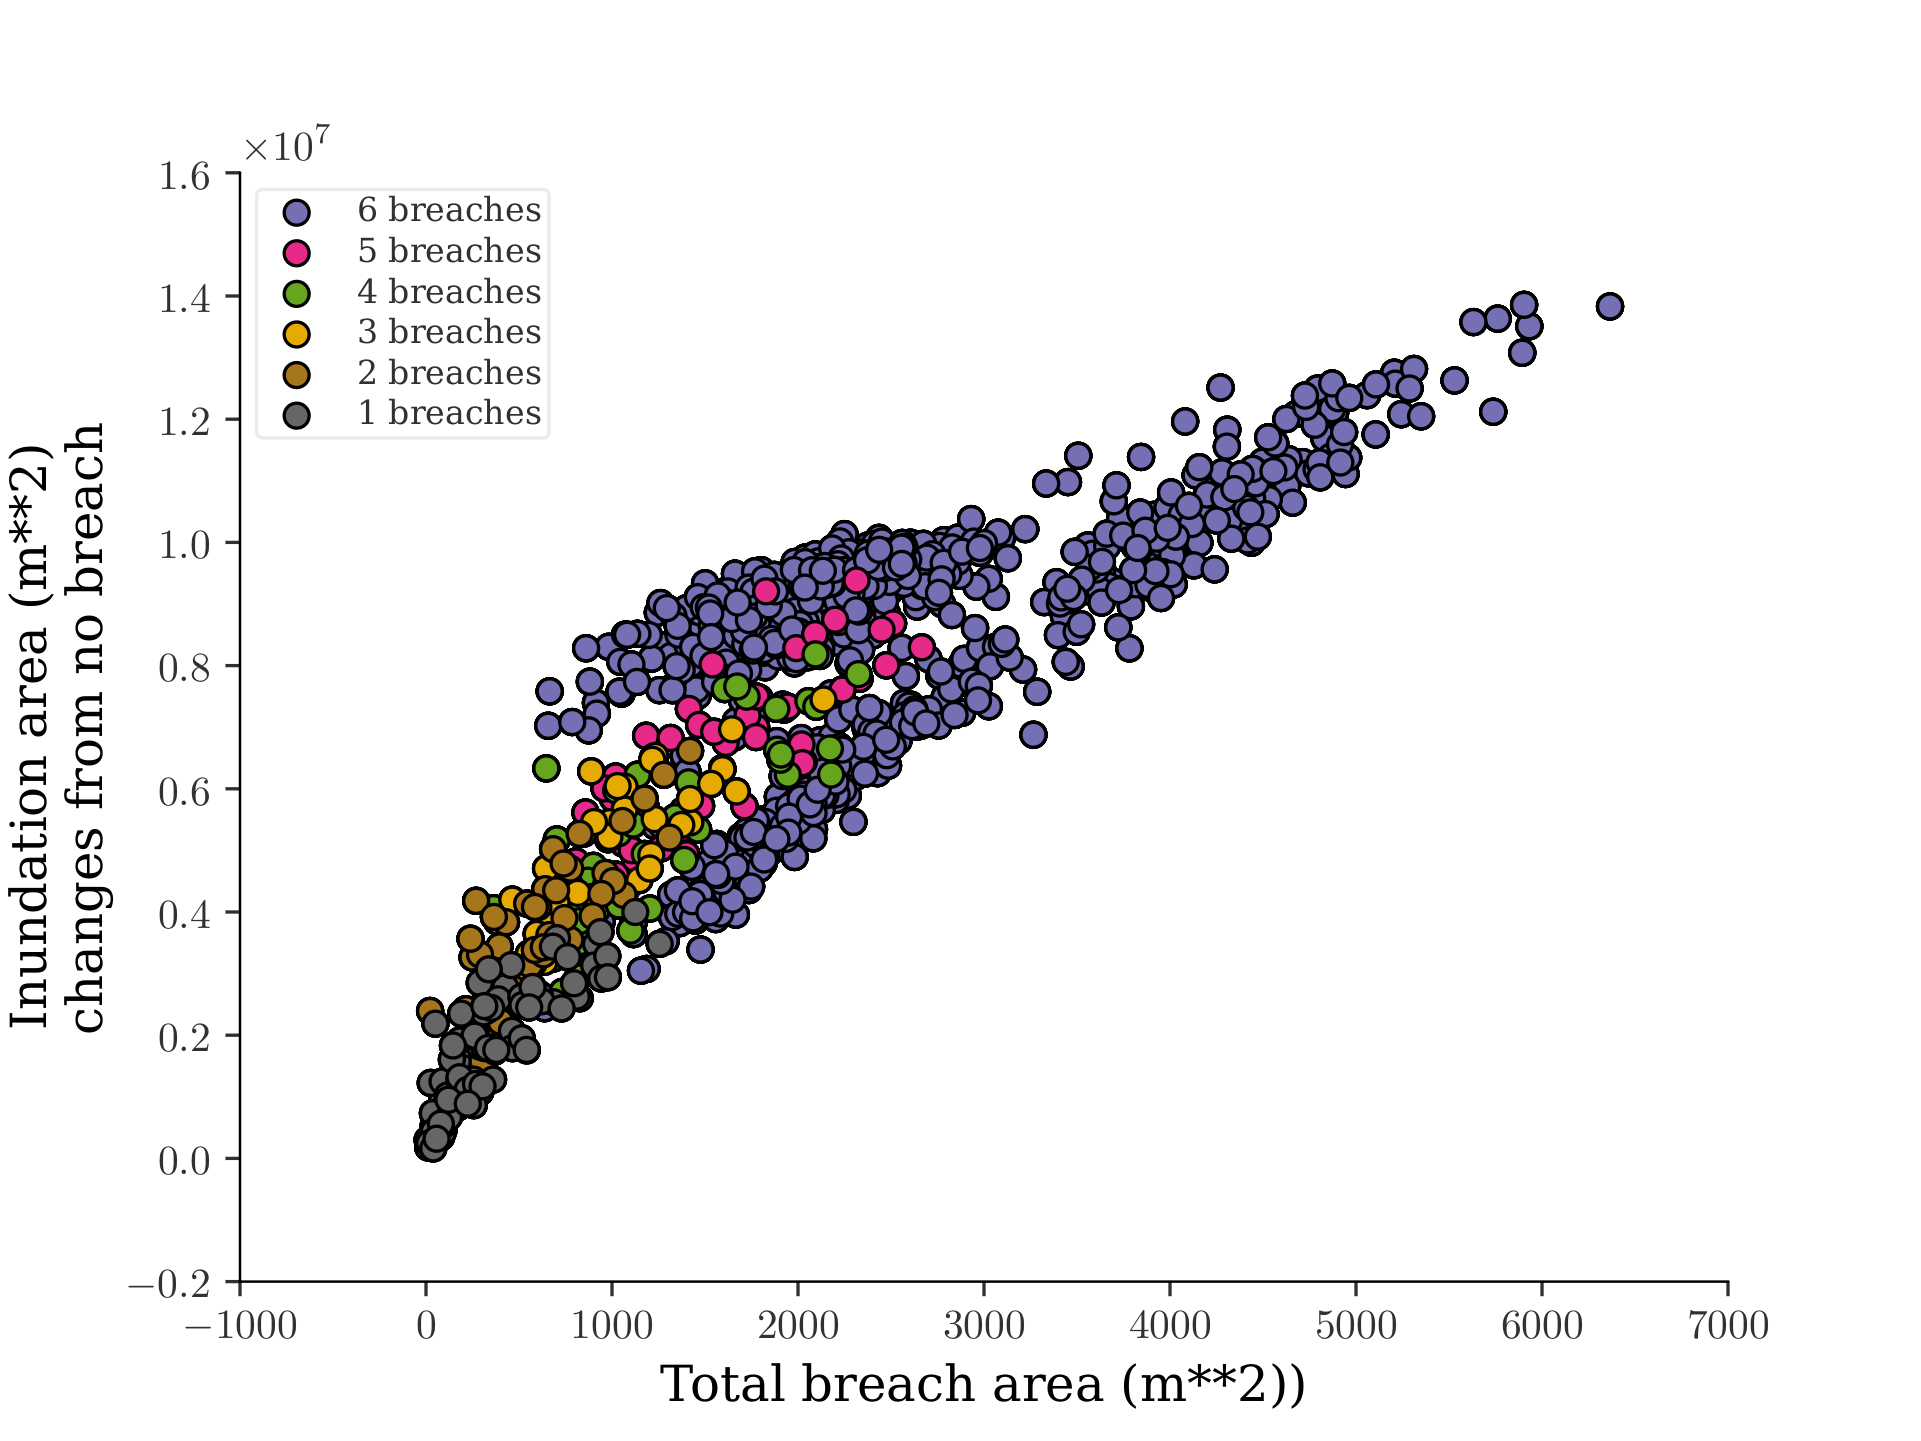
\includegraphics[width=0.75\textwidth]{images/inundation_x_total_breach_area.png}
    \caption{Total breach area vs. Inundation}
    \label{fig3}
\end{figure}

Figures 4-7 illustrate that different inundation patterns are correlated to number and size of breaches. Figure 4 is a no breach scenario which looks very similar in surge and inundation distribution to the minimum inundation which has only a single small breach. There are only approximately 500 different wet vs. dry cells between these two, which is 163,000 square meters or .1632 square kilometers of inundation. The scenario that comes closest to the mean of all the inundation is four moderate sized breaches, and the storm surge depths in the bay and inundation are very different than either the minimum or no breach scenarios. With higher flooding potential in the river drainages and along the lower elevation coastlines. Lastly the maximum inundation scenario shows all six breaches with very large areas, which merges two of the breaches on the eastern side of the inlet. This scenario again shows further flooding in the river drainages and along the coastline, although at the bay scale it is more challenging to differentiate from the mean.

\begin{figure}
    \centering
    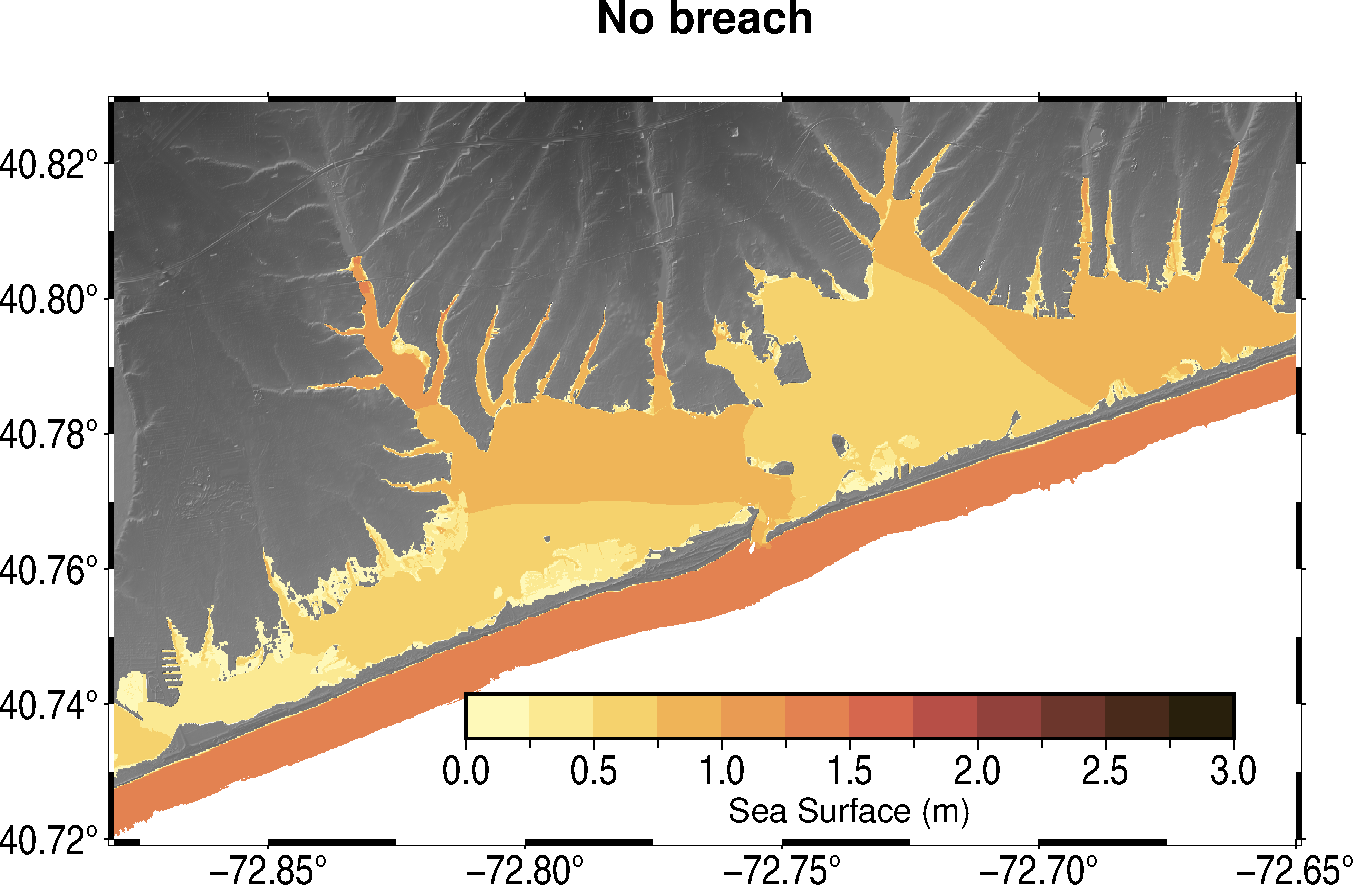
\includegraphics[width=0.75\textwidth]{images/Nobreach.pdf}
    \caption{Map of storm surge for a no breach scenario}
    \label{fig4}
\end{figure}
\begin{figure}
    \centering
    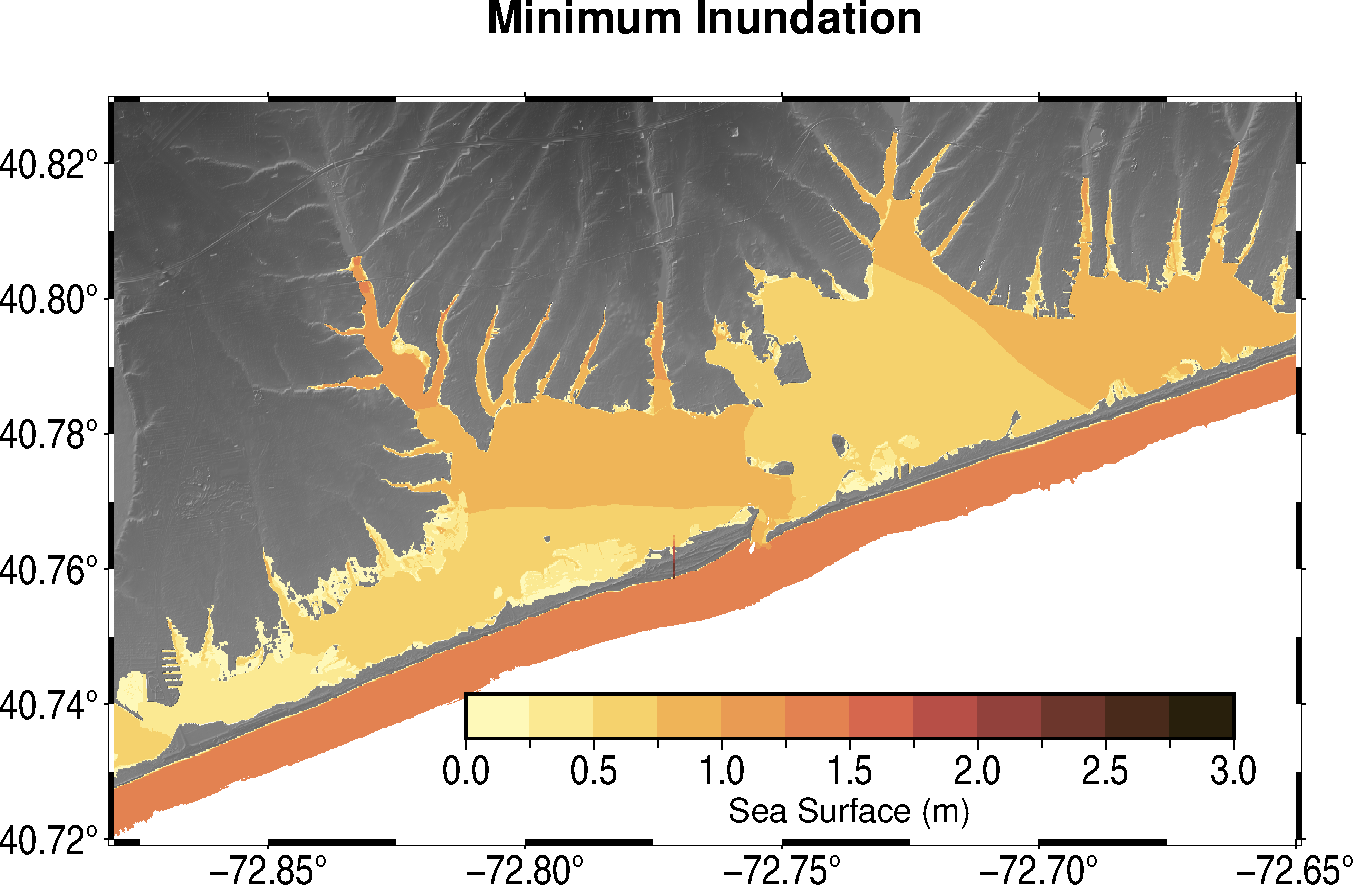
\includegraphics[width=0.75\textwidth]{images/min_inundation.pdf}
    \caption{Map of storm surge for the minimum inundation}
    \label{fig5}
\end{figure}
\begin{figure}
    \centering
    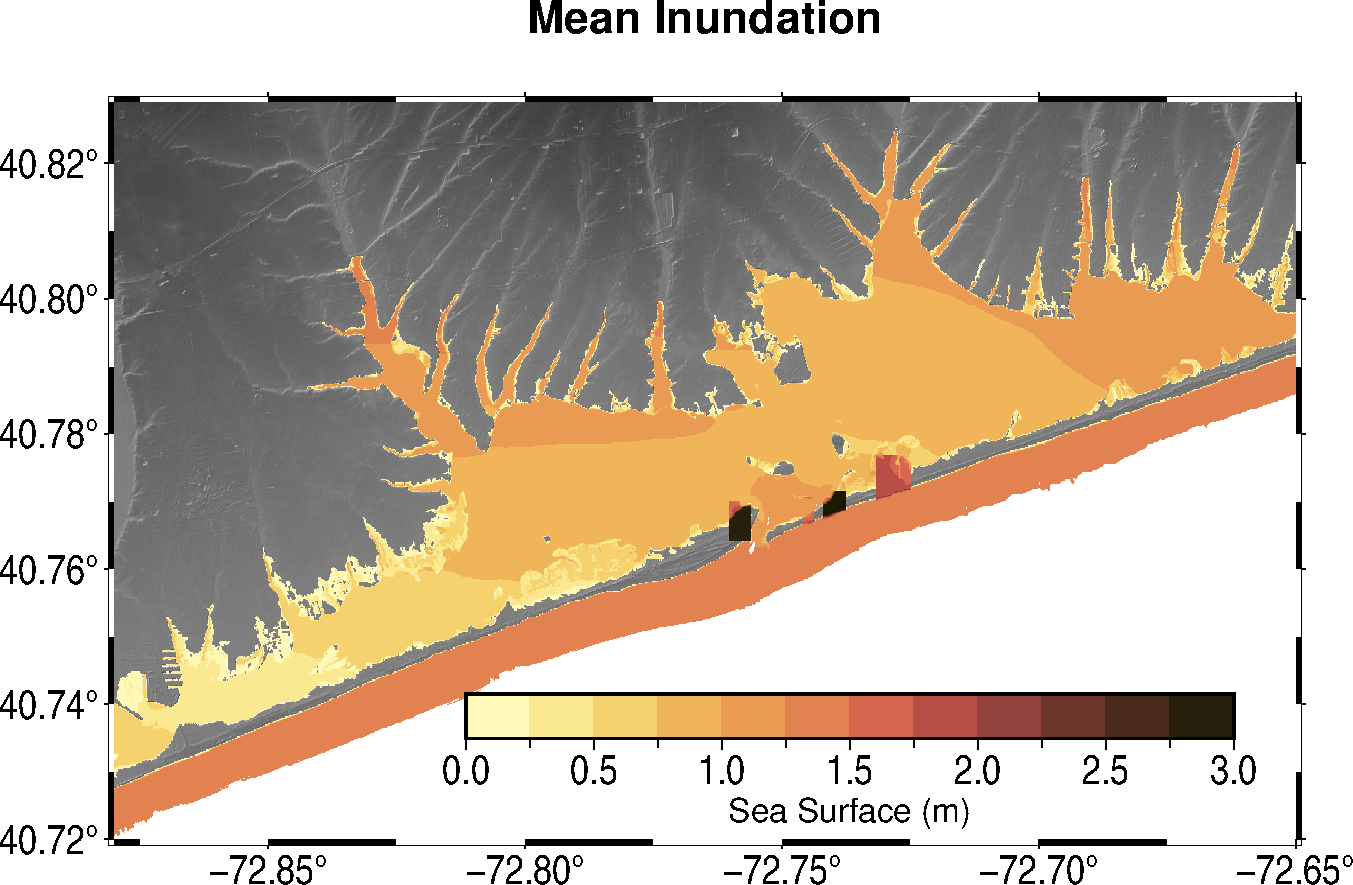
\includegraphics[width=0.75\textwidth]{images/mean_inundation.pdf}
    \caption{Map of storm surge for the mean inundation}
    \label{fig6}
\end{figure}
\begin{figure}
    \centering
    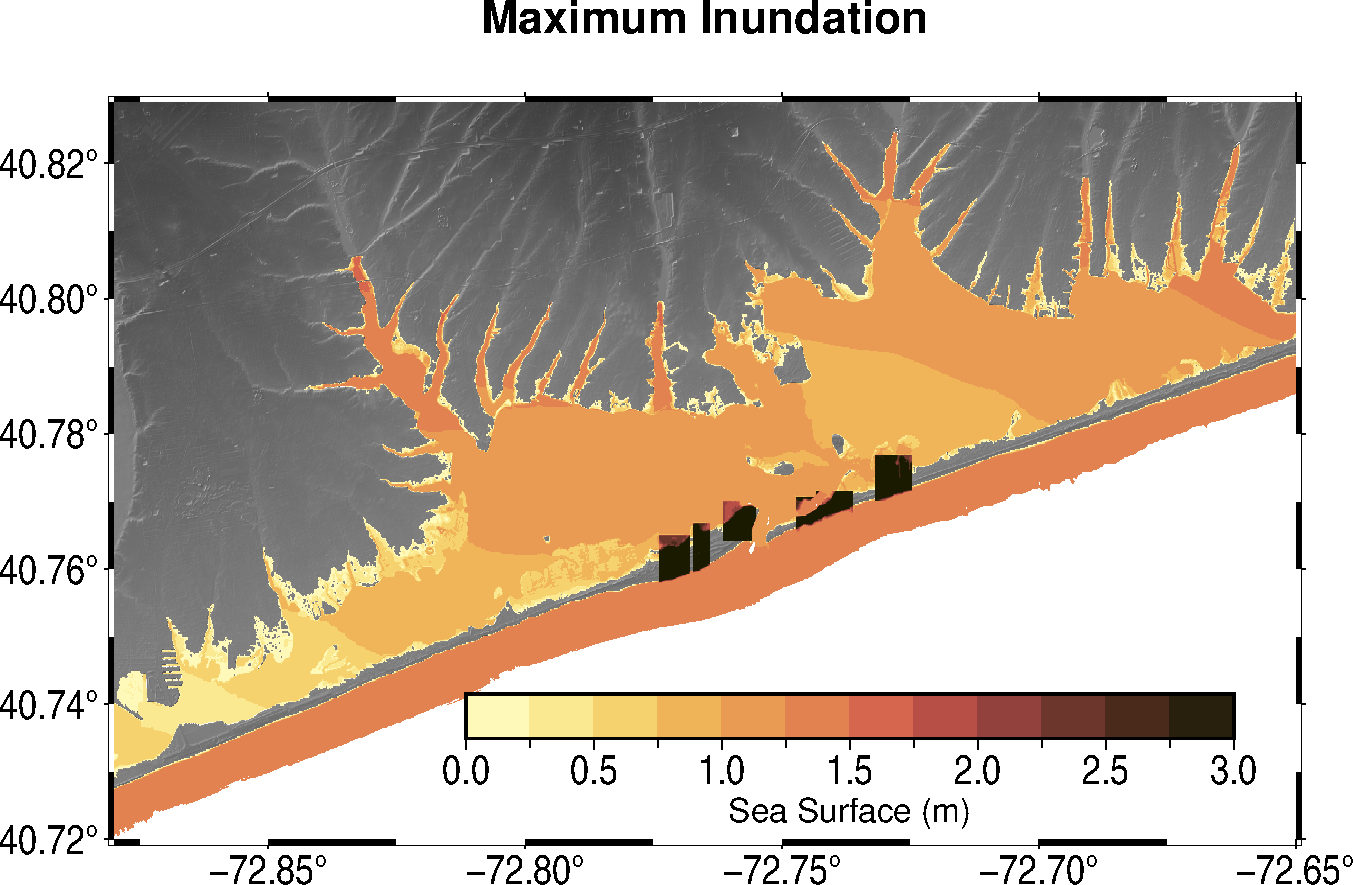
\includegraphics[width=0.75\textwidth]{images/max_inundation.pdf}
    \caption{Map of storm surge for a max inundation}
    \label{fig7}
\end{figure}
% Discuss here about total number of breaches and breach locations varying when that data is analyzed.

% Highlite fgmax overlay in google earth to show where shoring up regions that are always inundated.
% Discuss depth of inundation on potential impacts like electrical lines

\section{Discussion}
Figure 3 illustrates that total breach area in the island is the strongest determining factor in higher mainland inundation. The depth variations show a higher mean inundation area due to some of the original breaches being very large, on the order to 20-100 times wider than the total depth. Single small breaches have less inundation potential than multiple small breaches or many breaches of mixed total area. Total width runs from 25 - 630 meters whereas total depth goes from 0 to -2.0 meters. 
Changing the locations of the breaches adn varying the number of breaches allowed to be the total number of viable sites on the island (around 295) shows...% Analyse the new simulations

\section{Conclusions}
Breaching of a barrier island during a hurricane shows a strong impact on mainland inundation. The number/(location?)/ and size of the breaches can change the inundation potential.

Future work: Run many (1000s) more simulations to be able to get a full distribution of data from depth/width breaching differences. Run more storms to show impacts from different approaches, storm sizes, storm structure (extratropical like Sandy?), storm speeds to perform the same analysis and gain a better understanding of breaching impacts. Do storms

\bibliography{ref}

\end{document}
